\documentclass{cmspaper}
\usepackage{graphicx}
\usepackage{rotate}
\usepackage{relsize}
\usepackage{amsmath}
\usepackage{amssymb}
\usepackage{cite}

\newcommand{\met} {\ensuremath{E\!\!\!\!/_T}}
\newcommand{\ttbar} {\ensuremath{t\bar{t}~}}
\newcommand{\ptll} {\ensuremath{P_T(\ell\ell)}}
\newcommand{\ptllres} {\ensuremath{P^{\rm res}_T(\ell\ell)}}

\begin{document}

%==============================================================================
% title page for many authors
%
\begin{titlepage}
\title{Implication of CMS results on phenomenological MSSM}

  \begin{Authlist}
    Maurizio Pierini
    \Instfoot{cern}{CERN}    
    Maria Spiropulu
    \Instfoot{caltech}{CERN \& California Institute Of Technology, Pasadena}    
    Filip Moortgat, Luc Pape
    \Instfoot{eth}{ETH, Zurich, Switzerland}
    Joseph Lykken
    \Instfoot{fnal}{Fermi National Accelerator Laboratory, Batavia, Illinois}
    Harrison Prosper, Sezen Sekmen
    \Instfoot{fsu}{Florida State University, Tallahassee}
    Sabine Kraml
    \Instfoot{lpsc}{LPSC, Grenoble}
    Sanjay Padhi
    \Instfoot{ucsd}{University of California, San Diego}
    
  \end{Authlist}

\begin{abstract}
We discuss the implication of CMS results on phenomenological MSSM (pMSSM). The pMSSM
consists of a huge number of free parameters, we address the parameters sensitive 
to the recent CMS studies in a statistical consistent manner. The sensitivity of one as a function 
of others are studied here. The results provide new constraints on parameters, sensitive to hadronic as well as 
multilepton final states using 35 pb$^{-1}$ of integrated luminosity.
\end{abstract}
\end{titlepage}

\section{Introduction}
\label{sec:intro}

After the successful operation of the Large Hadron Collider (LHC) and the CMS detector
in 2010 and 2011, and with good prospects for the future, the LHC is now ready to shed light on a number 
of open questions in Particle Physics 
such as the mechanism of electroweak (EW) symmetry breaking, or the 
new physics, Beyond the Standard Model (BSM), that stabilizes the EW scale. 

A wealth of theories that extend the Standard Model have been put forth during the past decades. Supersymmetry (SUSY) is
arguably the best motivated BSM theory --- and certainly the most 
thoroughly studied. 
Indeed, searches for SUSY are among the primary objectives of the 
CMS experiment. SUSY is exceedingly popular not 
only for its theoretical beauty but also because SUSY phenomenology 
is extremely rich, 
%in fact is can mimic almost any other new physics scenario. 
leading to a large variety of possible new signals at the LHC. 
In spite of this, the majority of SUSY studies focus on a very special 
setup: the so-called Constrained Minimal Supersymmetric Standard Model (CMSSM). 
This was justified in the preparation for discoveries as the CMSSM, 
having just a handful of new parameters, is very predicive. However, 
the simplifying assumption of universality at the GUT scale lacks a sound 
theoretical motivation. Consequently, the CMSSM should be regarded as a showcase 
model. When it comes to interpreting experimental results, it is reasonable and interesting to do this within the CMSSM because it 
provides (to some degree) an easy way to show performances, 
compare limits or reaches, etc. However, the interpretation of experimental results in the 
$(m_0,m_{1/2})$ plane risks imposing unwarranted constraints on SUSY, as many 
mass patterns and signatures that are possible a priori are not covered in the CMSSM. 
The same problem arises in any analysis that assumes a particular 
SUSY breaking scheme. 

In this document, we therefore introduce a different approach, which uses only 
minimal assumptions on the underlying SUSY parameters. In particular, given the absence of experimental guidance, we choose
not to rely on a particular SUSY breaking scheme.
Instead, we use a 19-dimensional 
parametrization of the MSSM, called the \emph{phenomenological MSSM} (pMSSM),
with parameters defined not at the GUT scale but instead at the SUSY scale 
(by convention the geometric mean of the two stop masses).
We demonstrate the feasibility of our approach by applying it to 
the 2011 CMS data-set corresponding to 1~fb$^{-1}$ of integrated luminosity.  
Using profile likelihoods, we combine 
the dijet $\alpha_T$ analysis, the opposite-sign dilepton 
analysis and the same-sign dilepton analysis and derive constraints 
on the SUSY particles with as few simplifying assumptions as possible.
Results from other SUSY analyses in CMS will be added as soon as they become available.

We first give the motivation to go beyond the CMSSM and work in 
a generic MSSM setup. After this, the pMSSM and its parametrization is defined. 
We then outline our analysis, giving details on the pMSSM points we have used, 
the detector simulation and the CMS analyses, and describe the statistical method based on 
profile likelihoods used for coping with the 19-dimensional model. Finally, we discuss our results and summarize our conclusions.


\section*{Appendix}
\label{sec:stat}
We describe the (frequentist) 
statistical procedures we have used in this study.  Suppose 
that our goal is to make a statement about the parameter $\theta_1$,
say the gluino mass
parameter $M_3$, independently of the remaining 18 pMSSM parameters. Since the 
expected signal $s$ is a function of  $d = 19$ parameters (see Sect.~(\ref{sec:pmssm}),
which we denote by $\theta = \theta_1,\cdots,\theta_{19}$,  we need to eliminate $d - 1$ of them from the likelihood function so that the latter becomes a function of $\theta_1$ only. In general, it is extremely difficult to do this in 
a frequentist calculation in a way that preserves \emph{exact} coverage over the entire parameter
space. However, let $L_p(\theta_1) \equiv L(\theta_1, \hat{\theta}_2(\theta_1), \cdots)$ be the 
1-dimensional \emph{profile likelihood}, that is, the function obtained by maximizing the likelihood function $L(\theta_1, \theta_2, \cdots, \theta_{19})$ with respect to $\theta_2,\cdots,\theta_{19}$ for \emph{fixed} $\theta_1$ and replacing the exact, but unknown, values of $\theta_2,\cdots,\theta_{19}$
by their maximum likelihood estimates (MLE),  $\hat{\theta}_2(\theta_1),\cdots,\hat{\theta}_{19}(\theta_1)$. 

Replacing exact values by estimates is clearly an approximation. We should therefore not
expect any procedure that uses this approximation to yield confidence limits and intervals
with exact coverage. However, in practice, 1-dimensional profile likelihoods created from
multi-parameter likelihood functions often perform
surprisingly well~\cite{James}.
Let $L_{max}$ be the maximum of the likelihood function $L(\theta)$ and let 
$\Lambda = L_p /  L_{max}$ be the likelihood ratio. 
If the partial derivatives with respect to $\theta_i$ of the likelihood function, $L(\theta)$, exist up to second order and they form a $d \times d$ non-singular matrix (the Hessian), 
the following result holds,
\begin{equation}
    W = -2\log\Lambda \rightarrow \chi^2,
\end{equation}
as the amount of data grows without limit. This is  Wilks theorem~\cite{Wilks, James}. For an 
approximate 95\% C.L. lower limit on $\theta_1$, we set $W = 1.64$, that is, $\Lambda = 0.44$,
and solve for the lower limit.

\subsection*{Non-parametric profiling algorithm}
The problem we need to solve is the following: for a fixed value of a parameter, say $Q$, we want to find 
the maximum value of the likelihood function when the latter is available only as a weighted swarm of points. The quantity $Q$ could be a pMSSM parameter, a predicted observable of a 
sparticle mass. Here, written as pseudo-code, is our algorithm for finding the profile likelihood:
\begin{verbatim}
1	pMSSMPOINTS, QBIN, Q = inputs()
2	NBOOTSTRAP = 100
3	profile = 0

4	repeat NBOOTSTRAP times:
	      
5	      POINTS = generateBootstrapSample(pMSSMPOINTS)
6	      histogram = histogramPoints(POINTS)
	
7	      DMAX = -1
8	      for point in POINTS:
	      
9	           if Q not in QBIN: continue
	      
10	           d = histogram.density(point)	      
11	           if d > DMAX: DMAX = d
	 
12	      profile = profile + DMAX
	        
13	 profile = profile / NBOOTSTRAP	 
14	 return profile	      
\end{verbatim}
\begin{itemize}
	\item[1] Get the pMSSM points, the bin $QBIN$ for which the profile likelihood
	is to be computed, and the value of $Q$.
	
	\item[6] Generate a $d$-dimensional histogram from current bootstrap sample.
	
	\item[9] Make sure $Q$ lies in desired bin $QBIN$.
	
	\item[10,11] Find largest density $DMAX$ so far.
	
	\item[12--14] Return average of estimates of profile likelihood.
\end{itemize}
The above algorithm is implemented in a class we developed called {\tt KDTProfileLikelihood}, which
makes use of the multi-dimensional histogrammer {\tt TKDTreeBinning} in Root.
The $d$-dimensional histogram is created through recursive binary partitioning of the parameter
space in such a way that bins have equal counts. The underlying data structure is 
a kd-tree~\cite{TKDTreeBinning}.

\subsection*{Comparison of kinematic quantities with Full Simulation}
\label{sec:compare}
We compare the important kinematic variables used for the study with the CMSSW 
Full simulation using LM1 benchmark point. Figures~\ref{fig:njetht},~\ref{fig:jetpteta},~\ref{fig:alphat}
shows that the simulation/reconstruction infrastructure used agree well with the full simulation.

\begin{figure}[htbp]
\begin{center}
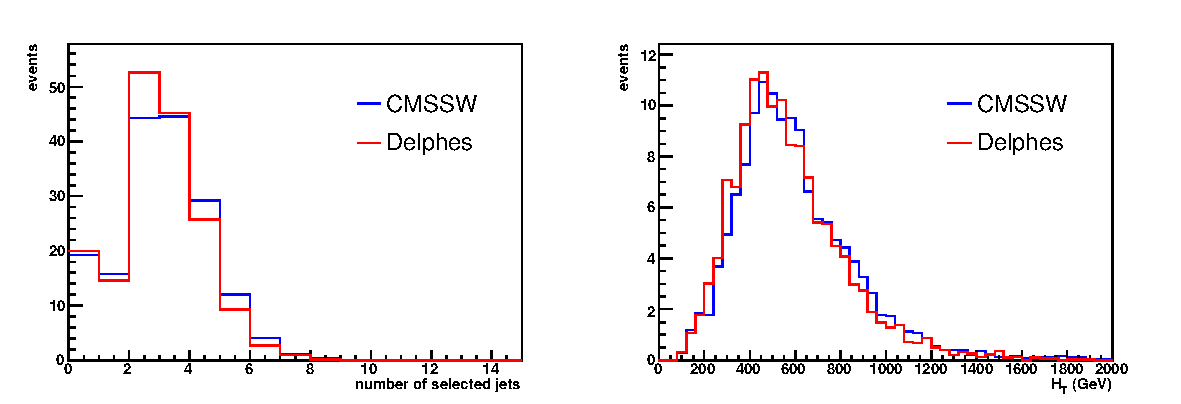
\includegraphics[height=5.5cm]{figs/njetht.pdf} 
\caption{Event distribution using CMSSW Full simulation along with Delphes for LM1 benchmark points, 
as a function of jet multiplicity (left) and $H_T$ (right)}
\label{fig:njetht}
\end{center}
\end{figure}


\begin{figure}[htbp]
\begin{center}
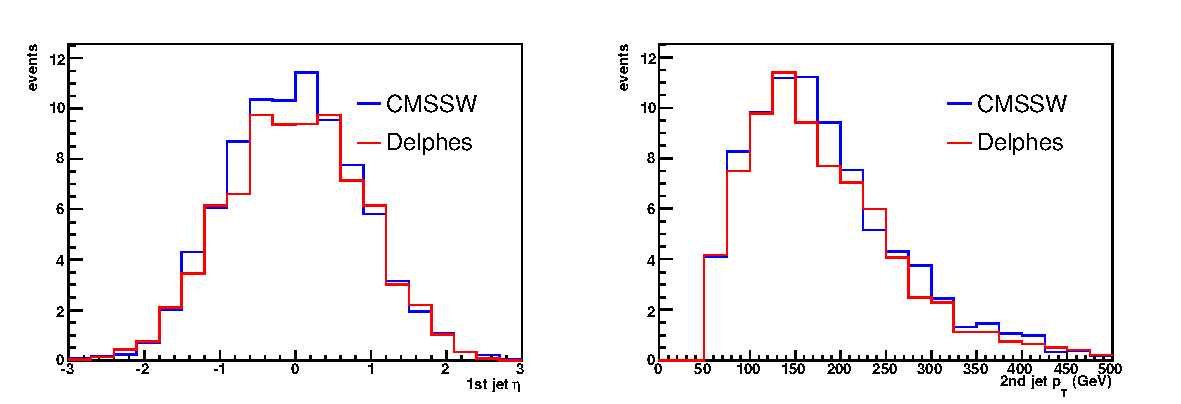
\includegraphics[height=5.5cm]{figs/jet1pteta.pdf} 
\caption{Event distribution using CMSSW Full simulation along with Delphes for LM1 benchmark points, 
as a function of pseudorapidity (left) and $p_T$ of the jets (right)}
\label{fig:jetpteta}
\end{center}
\end{figure}

\begin{figure}[htbp]
\begin{center}
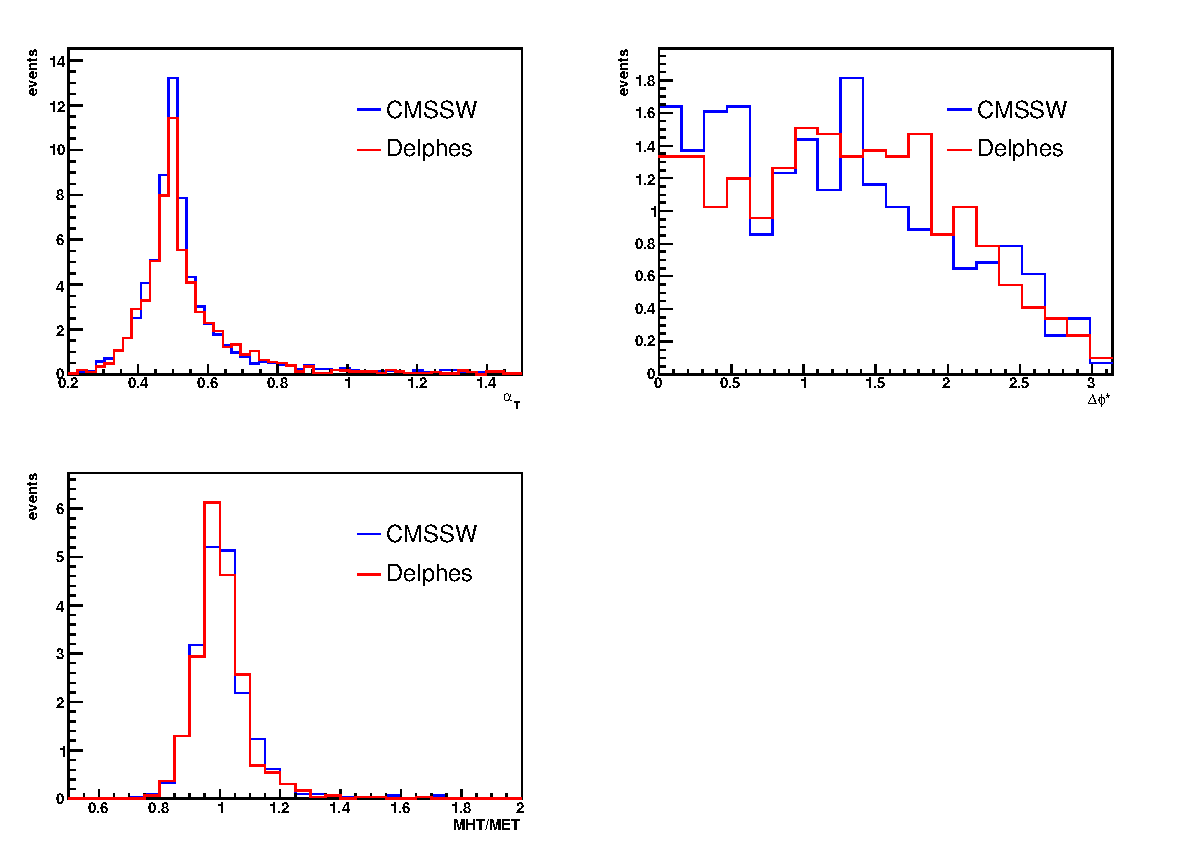
\includegraphics[height=9.cm]{figs/alphat.pdf} 
\caption{Event distribution using CMSSW Full simulation along with Delphes for LM1 benchmark points, 
as a function of $\alpha_{T}$ (top left), $\Delta \phi^{*}$ (top right) and MHT/MET (bottom)}
\label{fig:alphat}
\end{center}
\end{figure}


%\begin{thebibliography}
%	\bibitem{Wilks}
%	S.S~Wilks, ``The large-sample distribution of the likelihood ratio for testing composite hypotheses,'' Ann. Math. Statist. {\bf 9}, 60-62 (1938).
%	
%	\bibitem{James}
%	F.~James, ``Statistical Methods in Experimental Physics,''  2nd Edition, (World Scientific, Singapore, 2008).
%	
%\end{thebibliography}

\section{Current experimental and theoretical constraints}
\label{sec:limits}

The most relevant constraints today are the [SUSY and Higgs] mass 
limits from LEP2 and the Tevatron, electroweak precision observables, 
the branching ratios of the decays 
$B\to X_s\gamma$ and $B_s\to \mu^+\mu^-$, the anomalous magnetic moment of the 
muon $(g-2)_\mu$, and the relic density of dark matter $\Omega h^2$.  
They are compiled in Table~\ref{tab:observables} (to be extended).

Other important constraints, which we are not yet taking into account, 
come from $m_W$, $A^{\rm FB}_b$ and $\Delta M_{b}$.


\begin{table}[h]\begin{center}
\begin{tabular}{| l | c | c || c | l |}
  \hline
  Observable & exp.\ constraint & ref. & add. theory error & ref. \\ 
  \hline
  $M_Z$ [GeV] & $91.1875\pm 0.0021$ 
              & \cite{Nakamura:2010zzi} & -- & \\
  $M_t$ [GeV] & $173.3\pm 1.1$ 
              & \cite{top:1900yx} & -- & \\
  $\mbmb$ [GeV] &  $4.19^{+0.18}_{-0.06}$ 
                & \cite{Nakamura:2010zzi} & -- & \\
  $\asmz$ & $0.1184\pm 0.0007$ & \cite{Nakamura:2010zzi} & -- & \\
          & or $0.1176\pm 0.002$ & \cite{Nakamura:2010zzi} & -- & \\
  \hline
  $m_h$ [GeV] & $\ge 114.4$ & \cite{Schael:2006cr} 
              & $\pm 1.5$ & \cite{Degrassi:2002fi} \\
  $\Delta a_\mu \times 10^{-10}$ 
       & $e^+e^-:$ $29.6\pm 8.1$ 
       & \cite{Davier:2010nc} & $\pm 2$ & \\
       & $\tau's:$ $15.7\pm 8.2$ 
       & \cite{xxx} &  & \\
  ${\rm BR}(b\to s\gamma)\times 10^{-4}$  
       & $3.55 \pm 0.24_{\rm stat}\pm 0.09_{\rm sys}$  
       & \cite{HFAG:2010qj}  & ? &  \\
  ${\rm BR}(B_s\to \mu^+\mu^-)$  
       & $\le 3.6 \times 10^{-8}$ & \cite{HFAG:2010qj} & ? &  \\
  $\Omega_{\rm DM} h^2$ 
       & $0.1123\pm 0.0035$ 
       & \cite{Jarosik:2010iu} 
       & ? &   \\
  SUSY masses & LEP2 limits 
              & \cite{lepsusy} 
	      & ? & \\
  \hline
\end{tabular}
\end{center}
\caption{\label{tab:observables} Important observables, to be used in the likelihood calculation. }
\end{table}


\section{Results}
\label{sec:results}

We present the results obtained by following the analysis path in Section~\ref{sec:analysis}, in terms of  plots of likelihood ratios $L_p / L_{max}$ as a function of each parameter of interest.  Further details on this ratio as a  measure can be found in the Appendix.  

Plots of the likelihood ratio $L_p/L_{max}$ are shown for the 19 input pMSSM parameters in Figures~\ref{fig:LRwcms_msq} to~\ref{fig:LRwcms_tbmu}.  Similarly Figures~\ref{fig:LRwcms_sq} to~\ref{fig:LRwcms_Higgs} show the likelihood ratio for the physical sparticle masses.  The relationships between the scalar SUSY breaking mass parameters and the physical scalar masses as well as those between the gaugino mass parameters and the physical gaugino masses should be noted.  The colored and shaded histograms in each plot depict the likelihood ratio before and after the inclusion of CMS results, respectively.  We observe that the CMS results indeed introduce a variation in the likelihood ratios, where the variation is more enhanced for some parameters/masses and milder for others.  

We see that all squark/slepton mass parameters and all squark/slepton masses shift upwards systematically after the addition of CMS results.  The gaugino mass parameter $M_3$ and the gluino mass also move up simultaneously due to the constraints coming from the di-jet $\alpha_T$ analysis.  An important aspect to note is that no significant change is observed in the distribution for the mass of $\tilde{\chi}^0_1$, which is the lightest supersymmetric particle (LSP), since neither a stringent $E^T_{miss}$ cut nor any other technique dedicated to constraining the $\tilde{\chi}^0_1$ mass were imposed in the analyses considered.  We are ability to observe this effect due
to the freedom offered by the pMSSM parameterization, in which neutralino/chargino masses are allowed to vary independently of the gluino mass.  Had the interpretation been done using 
the CMSSM, we would be influenced by the strict gaugino mass relationship described in Section~\ref{sec:motivation}, and the $\tilde{\chi}^0_1$ mass would be forced to move upwards along with the gluino mass.

Figure~\ref{fig:LRwcms_omg} shows $L_p/L_{max}$ for the dark matter relic density calculated using {\tt micrOMEGAs 2.4}~\cite{Belanger:2006is} assuming $\tilde{\chi}^0_1$ is the LSP and the dark matter candidate.  It must be noted that Berger {\it et al.} imposed the WMAP upper limit $\Omega_{\tilde{\chi}^0_1}h^2 \le 0.1210$ as a constraint on the points.  Information from CMS does modify the distribution, however the effect is not sufficient to impose a concrete constraint on $\Omega_{\tilde{\chi}^0_1}h^2$.  This is of course related to the result on the $\chi^0_1$ mass.

Finally, Figures~\ref{fig:LRwcms_EWobs_s1} and~\ref{fig:LRwcms_EWobs_s2} show distributions for low energy observables as predicted by the pMSSM, calculated using {\tt micrOMEGAs 2.4} and {\tt Superiso 2.7}~\cite{Mahmoudi:2008tp}.  We again note that the constraints based on experimental measurements for a subset of these observables were imposed
by Berger {\it et al.} in their selection of the pMSSM points.  Similarly to the case for the relic density, the 2010 CMS measurements do not yet allow us to constrain these observables further.  However, the prospect of making statements on the predictions for low energy observables in the presence of more data and diverse analysis channels stands out as a strong motivation in favor of interpreting the data within the framework of supersymmetry.

The results we have presented in this Note, with only 35 pb$^{-1}$ of CMS data, show that even with a modest amount of data, we are able to start making inferences of a general nature
about supersymmetry. 
%on a sufficiently generic and well-motivated construction of supersymmetry.  
Therefore, we anticipate that at least with an order of magnitude more data, the approach we have developed will allow us to make definitive statements about a broad class of supersymmetric models.  
This is only the starting point in a vast landscape of investigation. In the near term, 
we will develop this approach further by considering the following:

\begin{itemize}
\item An improved treatment of the constraints from the EW observables.  We shall replace the box-like likelihood of Berger {\it et al.} by a more appropriate likelihood function.
\item A significant increase in the sample of pMSSM points. 
\item Inclusion of a wider range of final states.
\item The development of a more quantitative treatment of the bounds on the pMSSM parameter space.
\end{itemize}


\begin{figure}[htbp]
\begin{center}
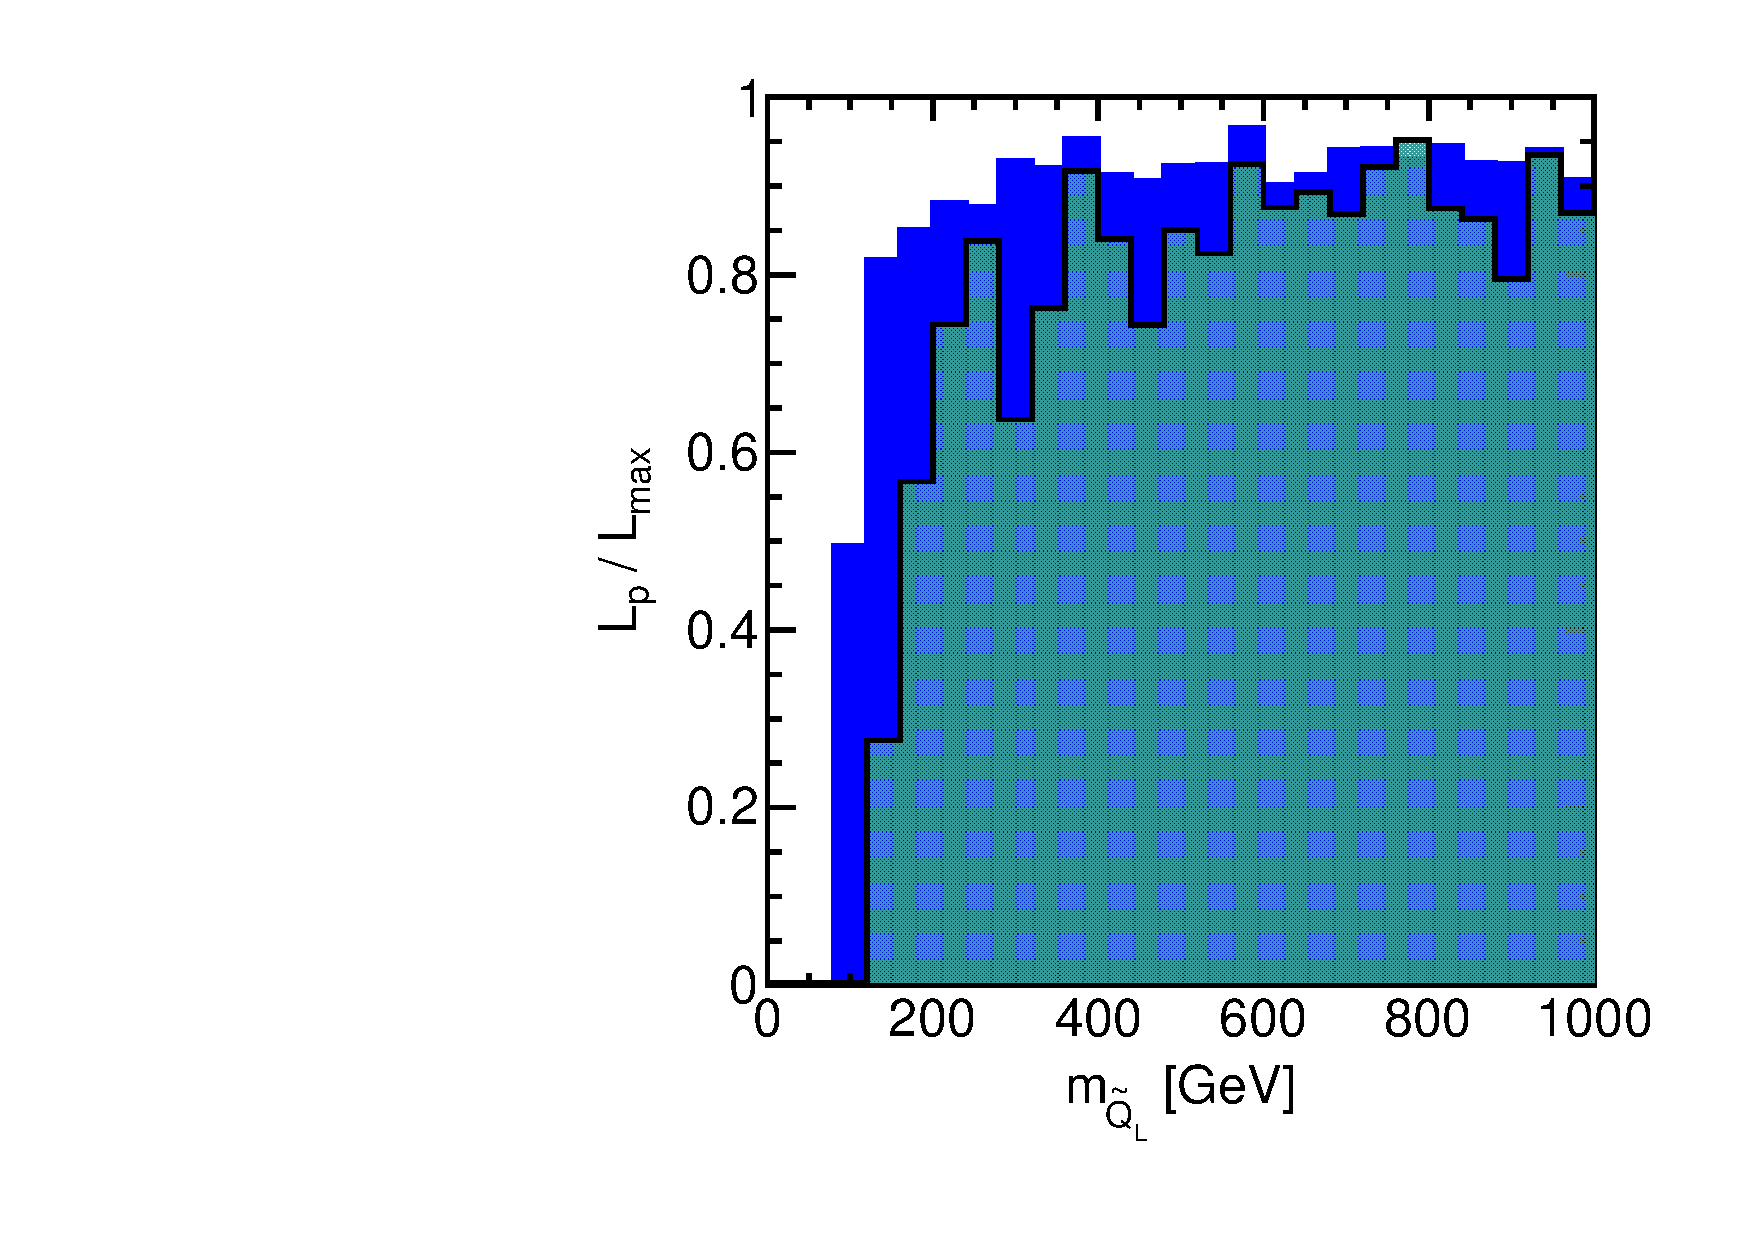
\includegraphics[height=5.5cm]{figs/fig_m_Q_L.pdf} 
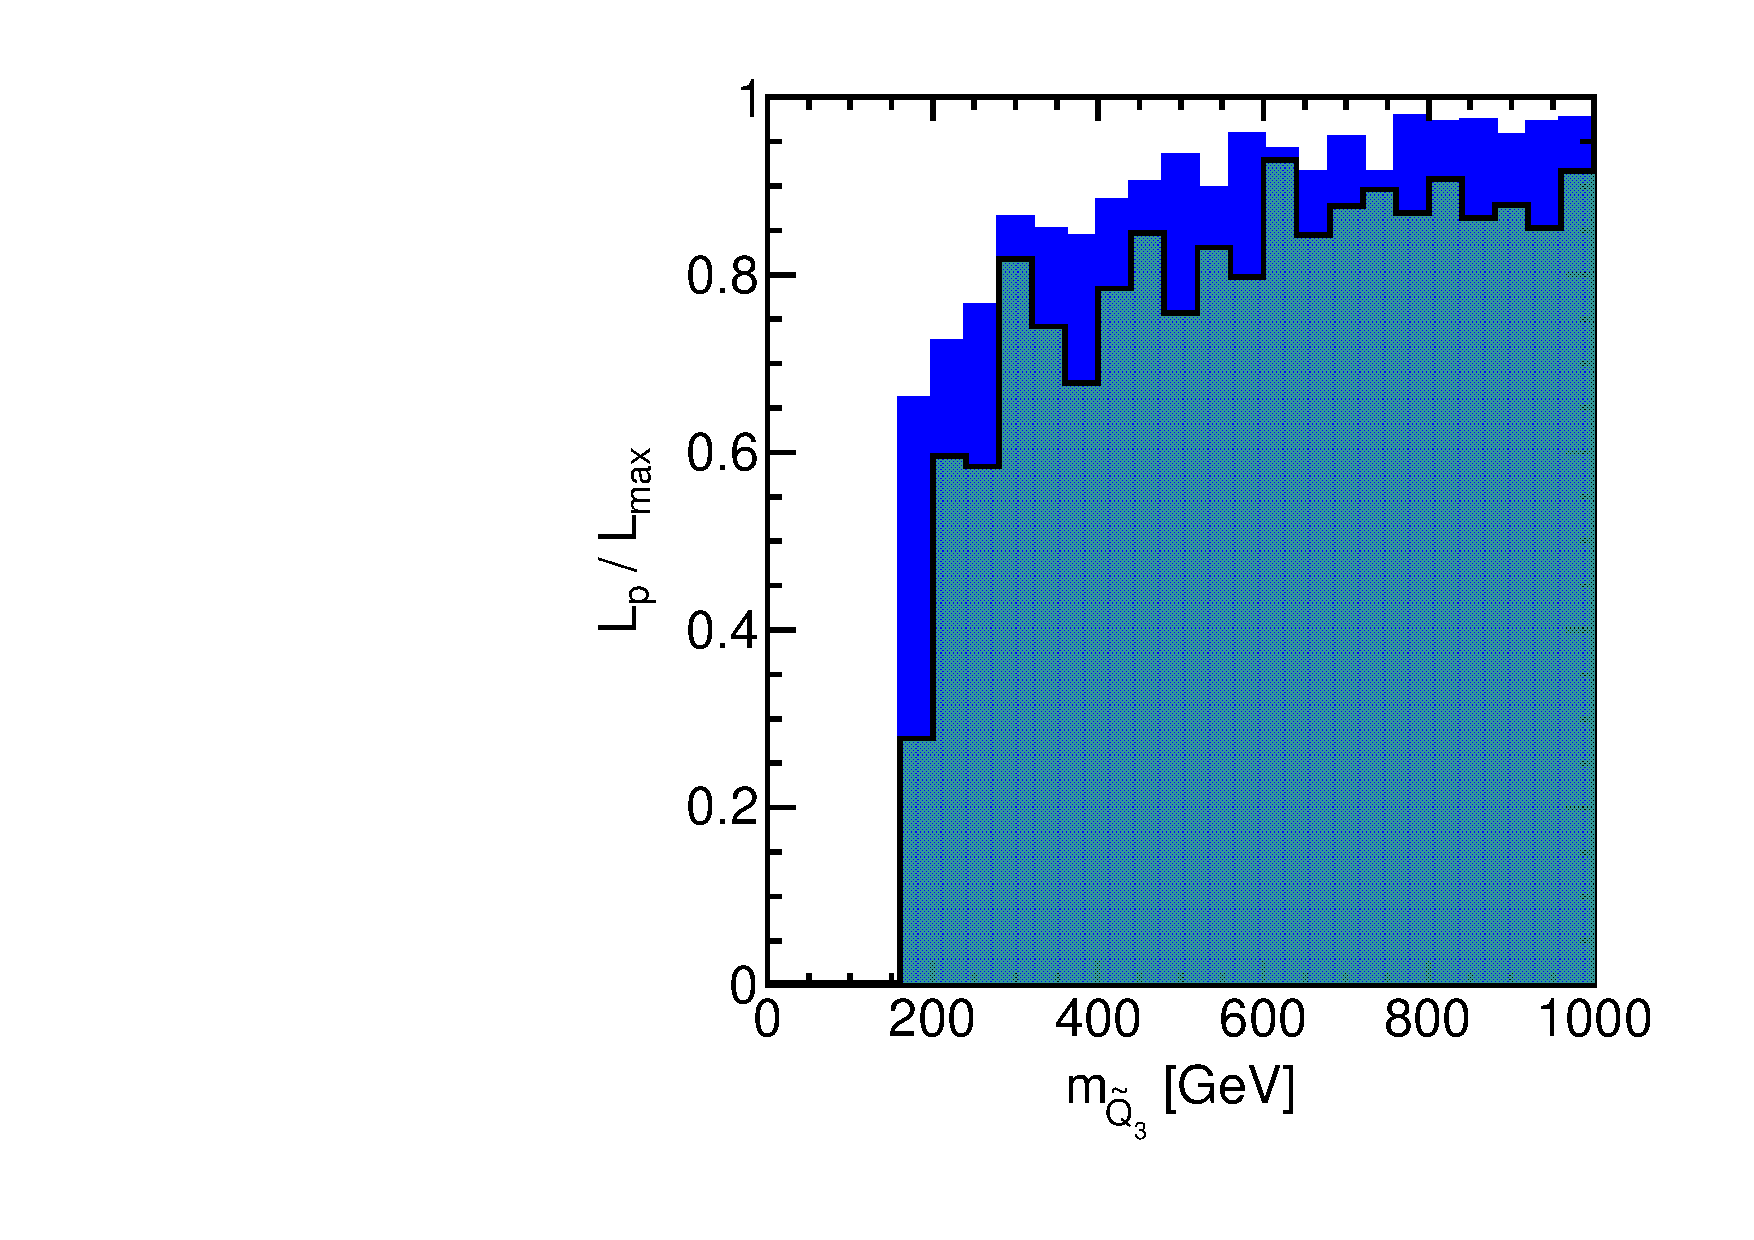
\includegraphics[height=5.5cm]{figs/fig_m_Q_3.pdf} \\
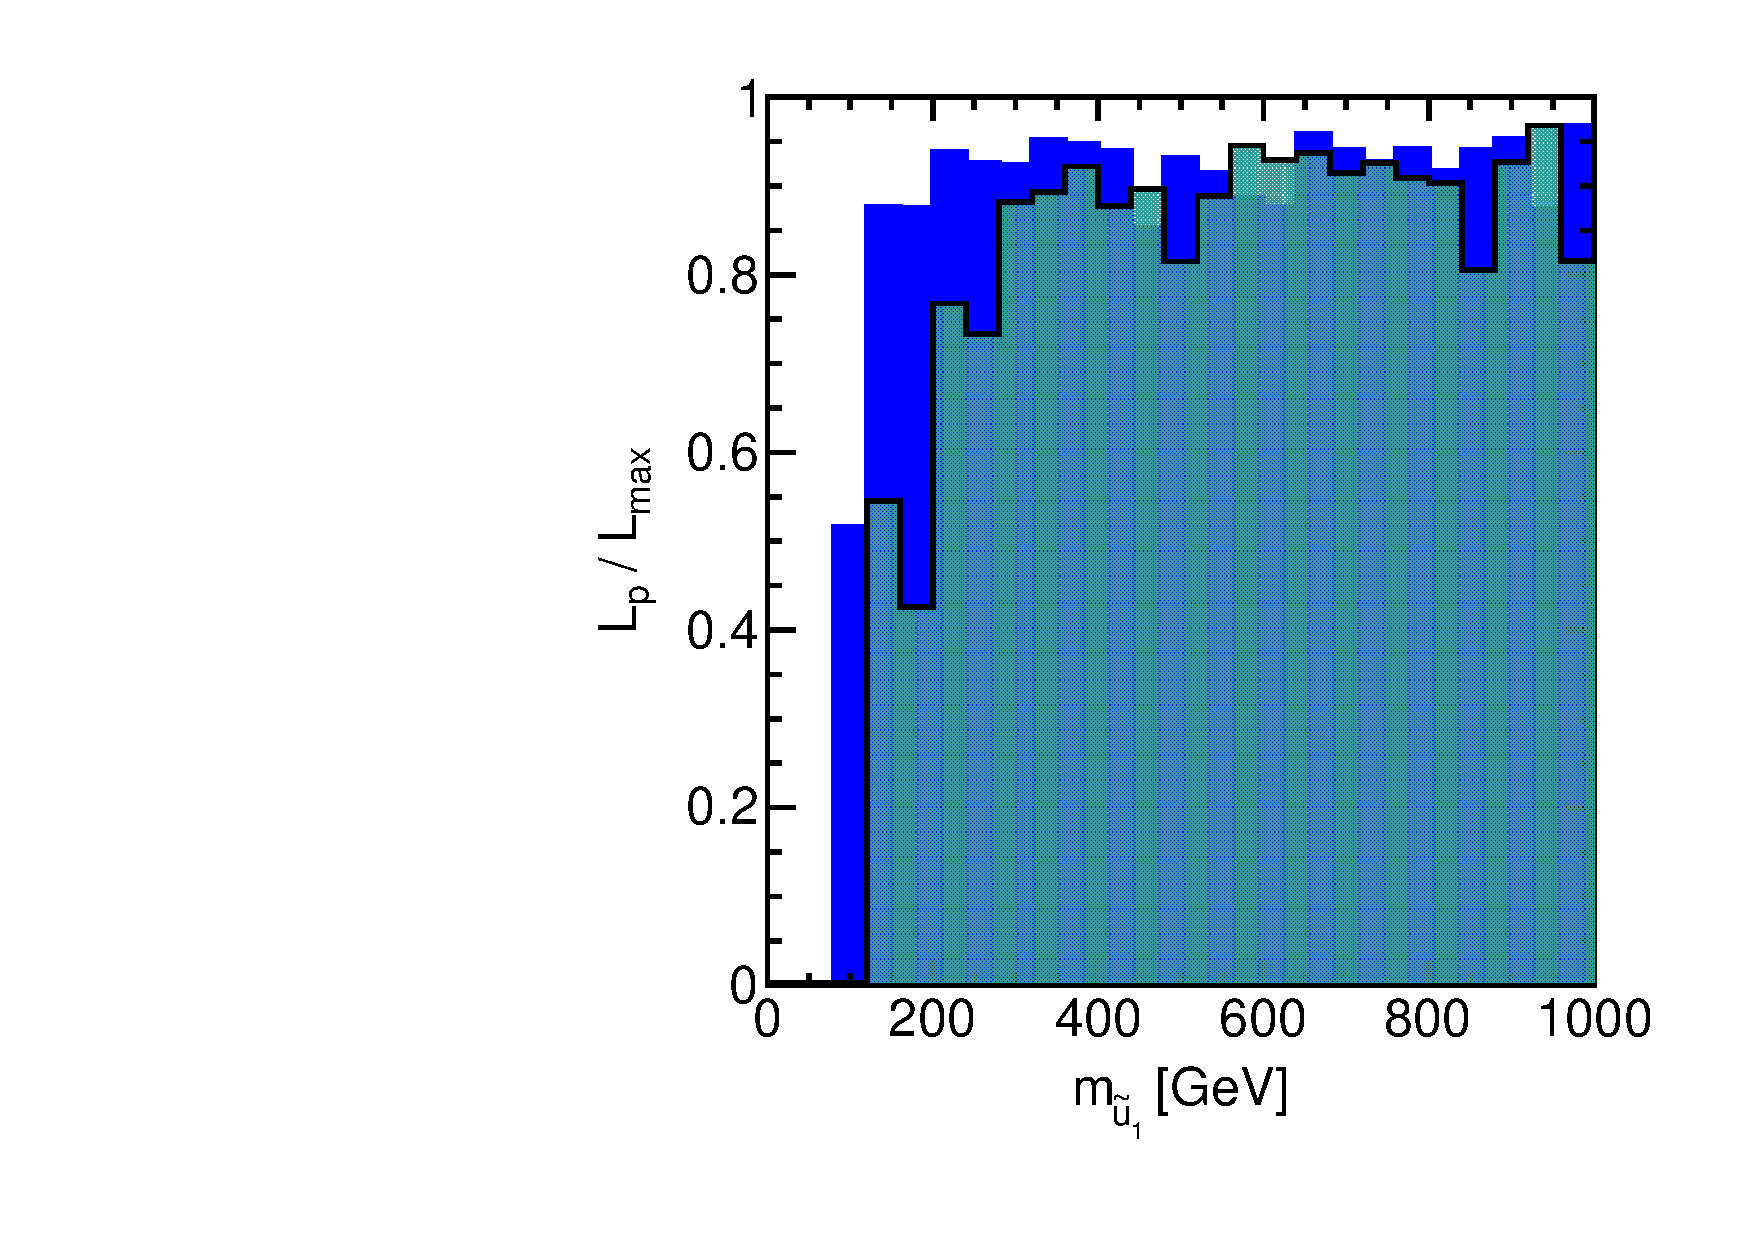
\includegraphics[height=5.5cm]{figs/fig_m_u_1.pdf}
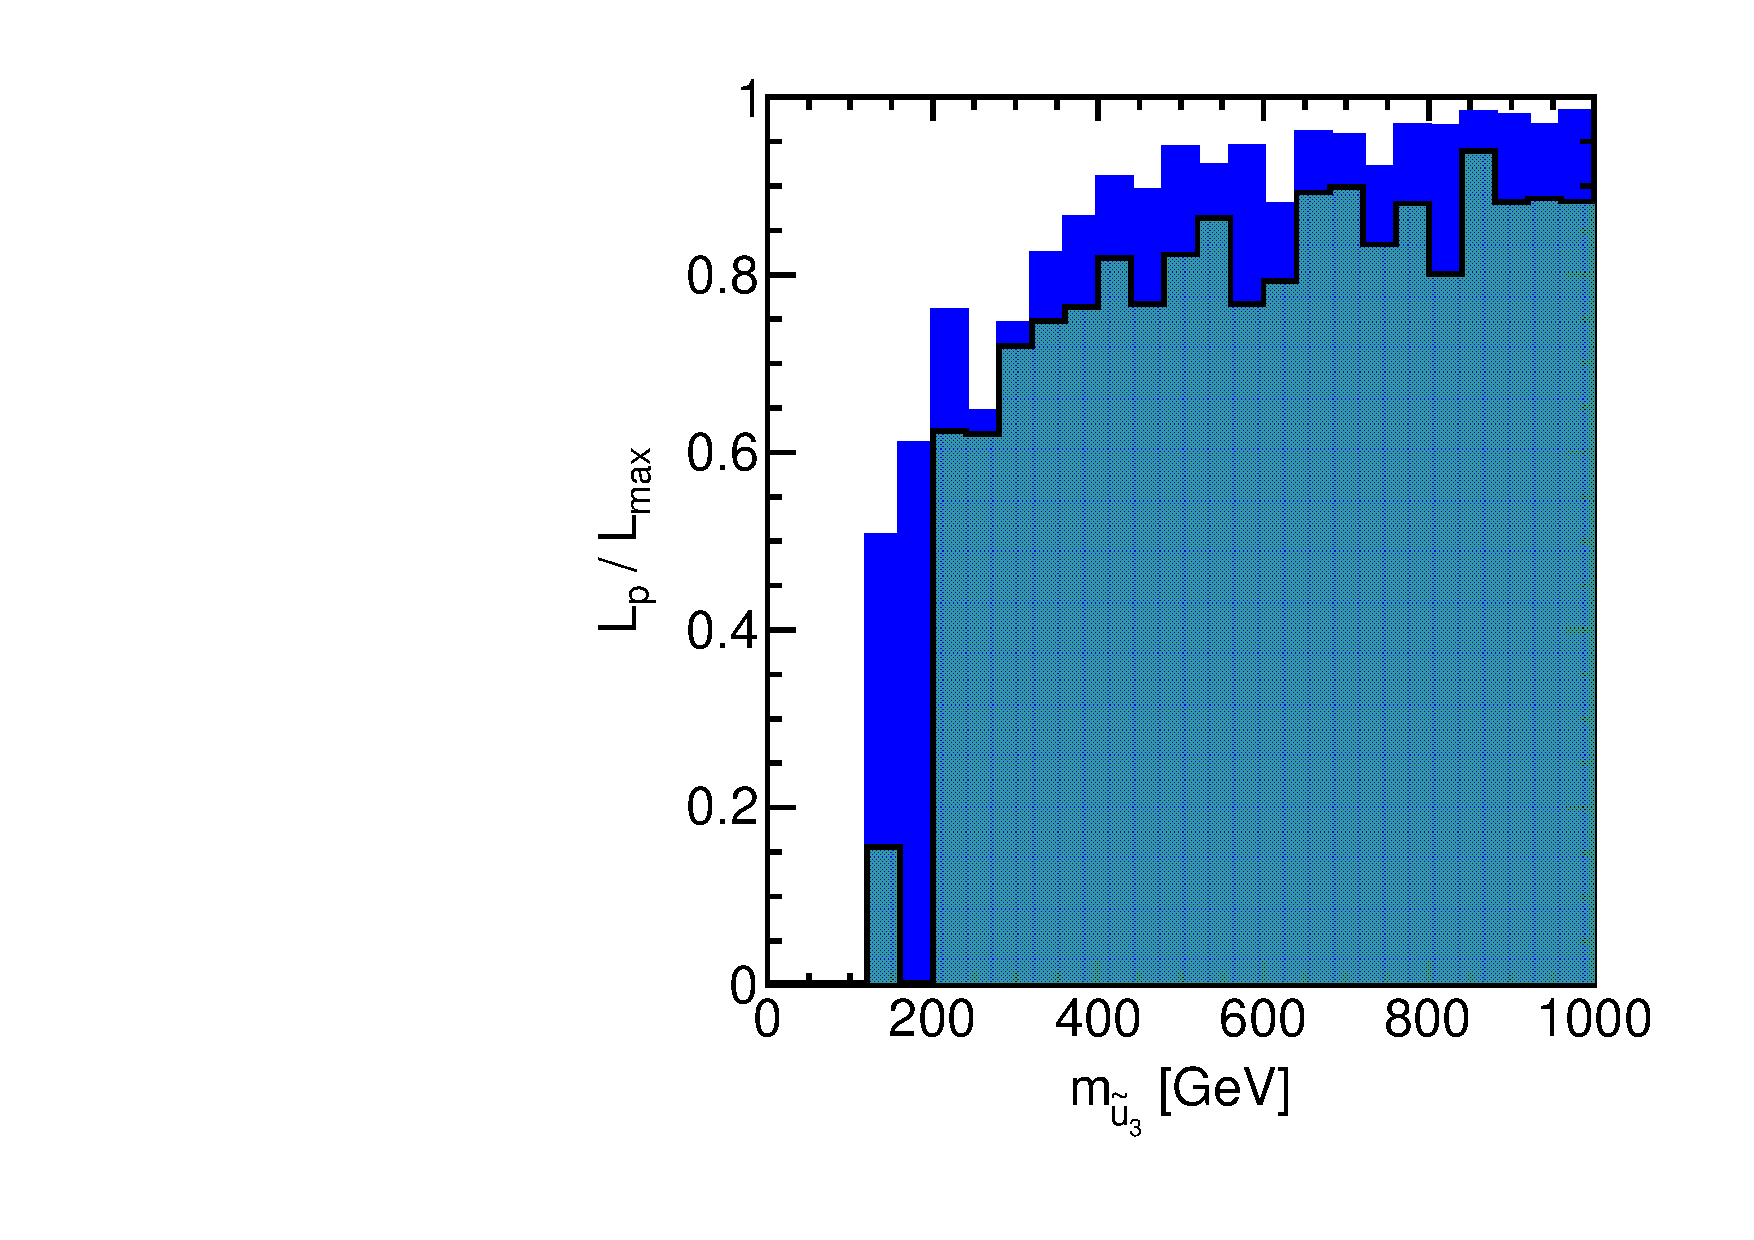
\includegraphics[height=5.5cm]{figs/fig_m_u_3.pdf} \\
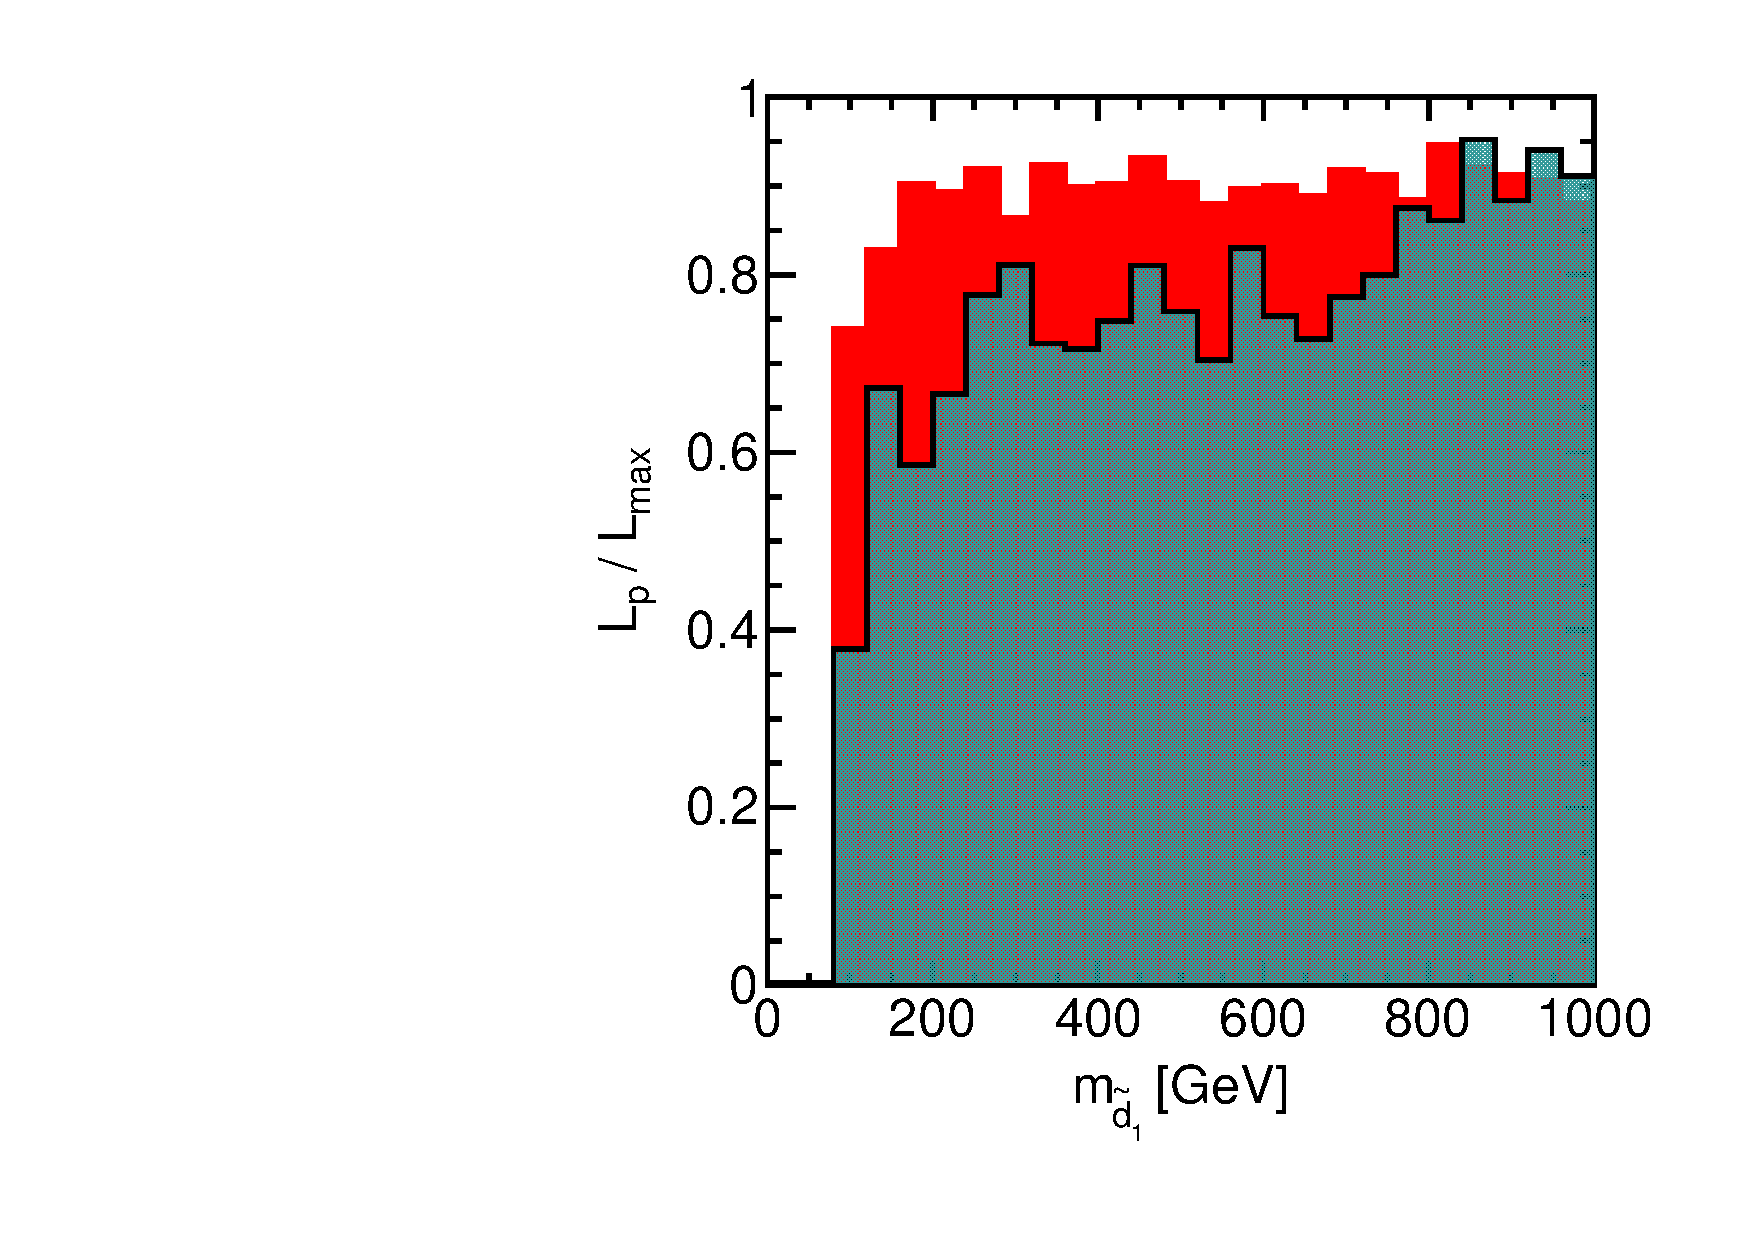
\includegraphics[height=5.5cm]{figs/fig_m_d_1.pdf}
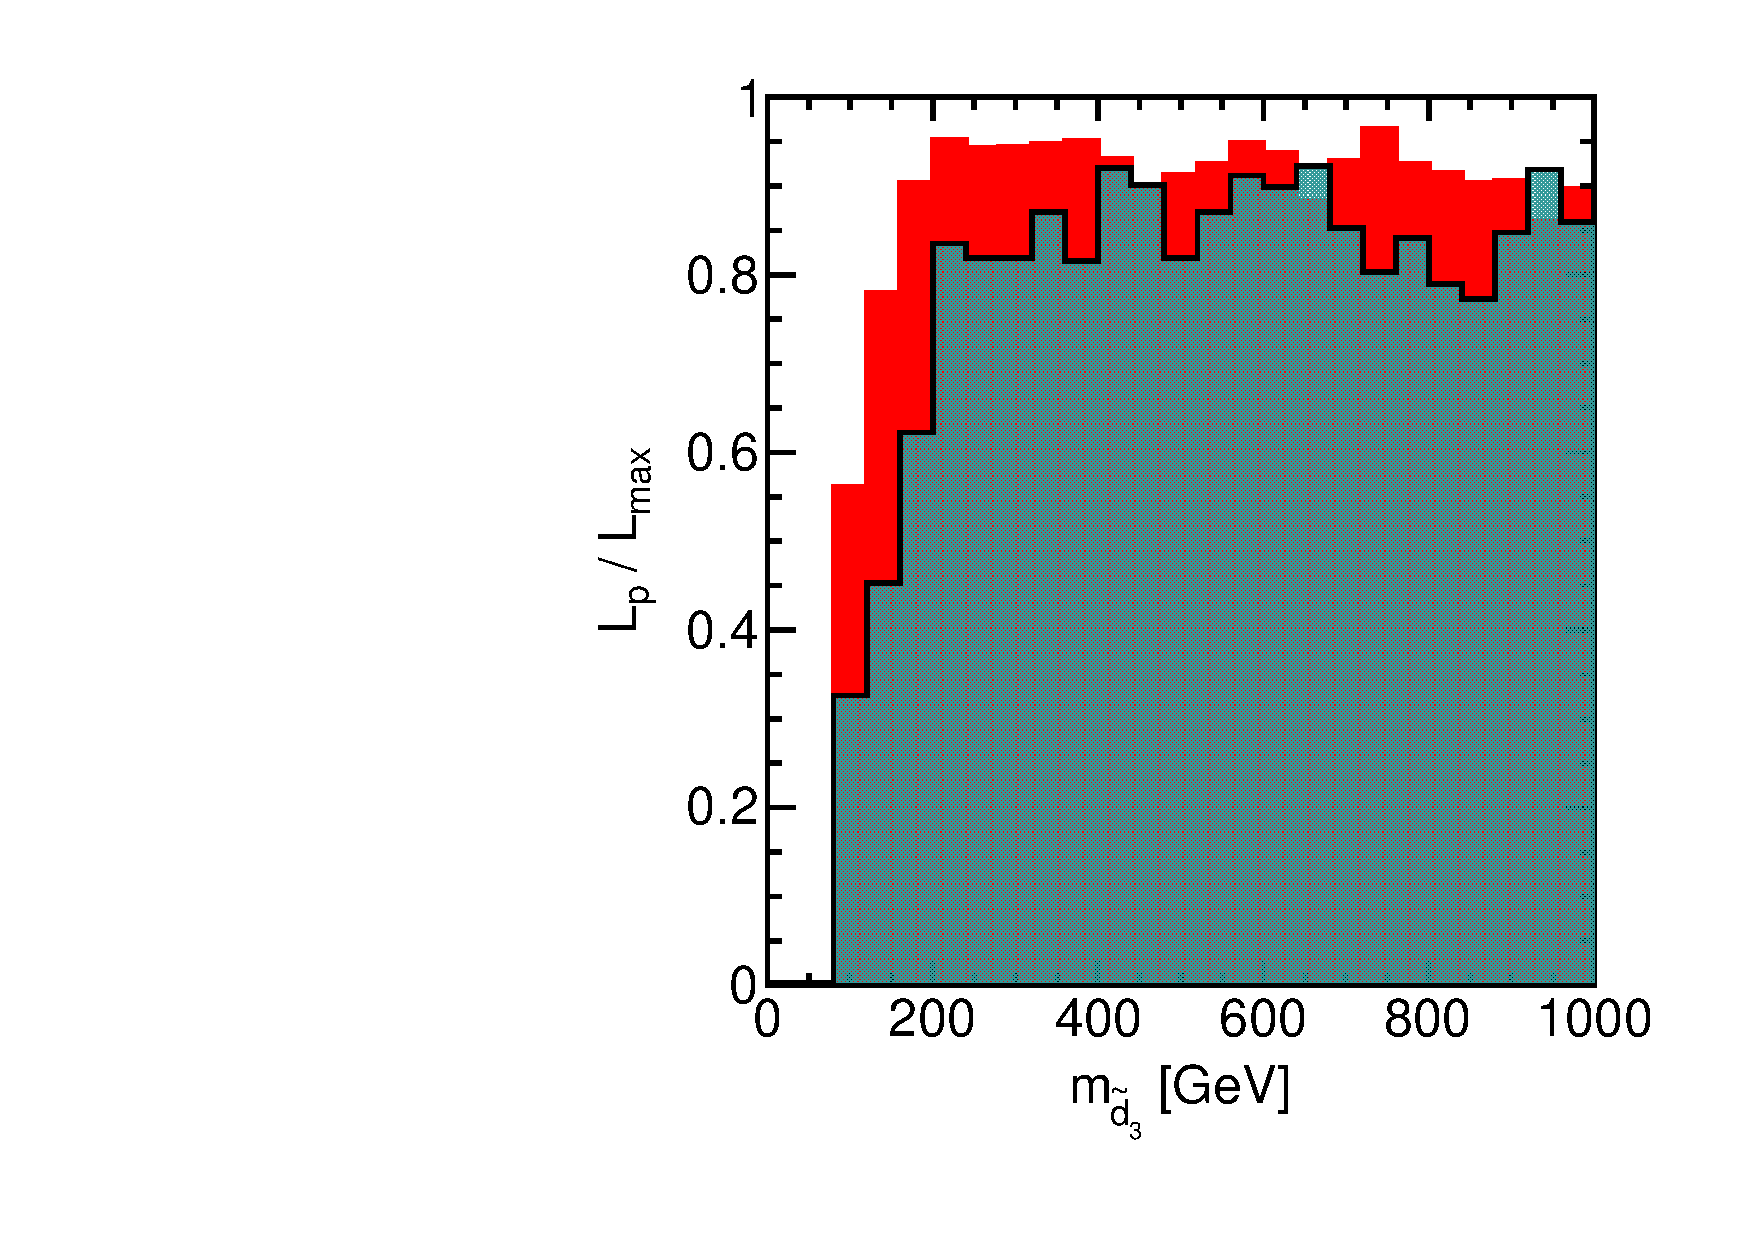
\includegraphics[height=5.5cm]{figs/fig_m_d_3.pdf}
\caption{Ratios of profile likelihood $L_p$ to maximum likelihood $L_{max}$ shown for the squark mass parameters at SUSY scale.  The colored and shaded histograms show the distributions before and after the inclusion of the CMS results.}
\label{fig:LRwcms_msq}
\end{center}
\end{figure}


\begin{figure}[htbp]
\begin{center}
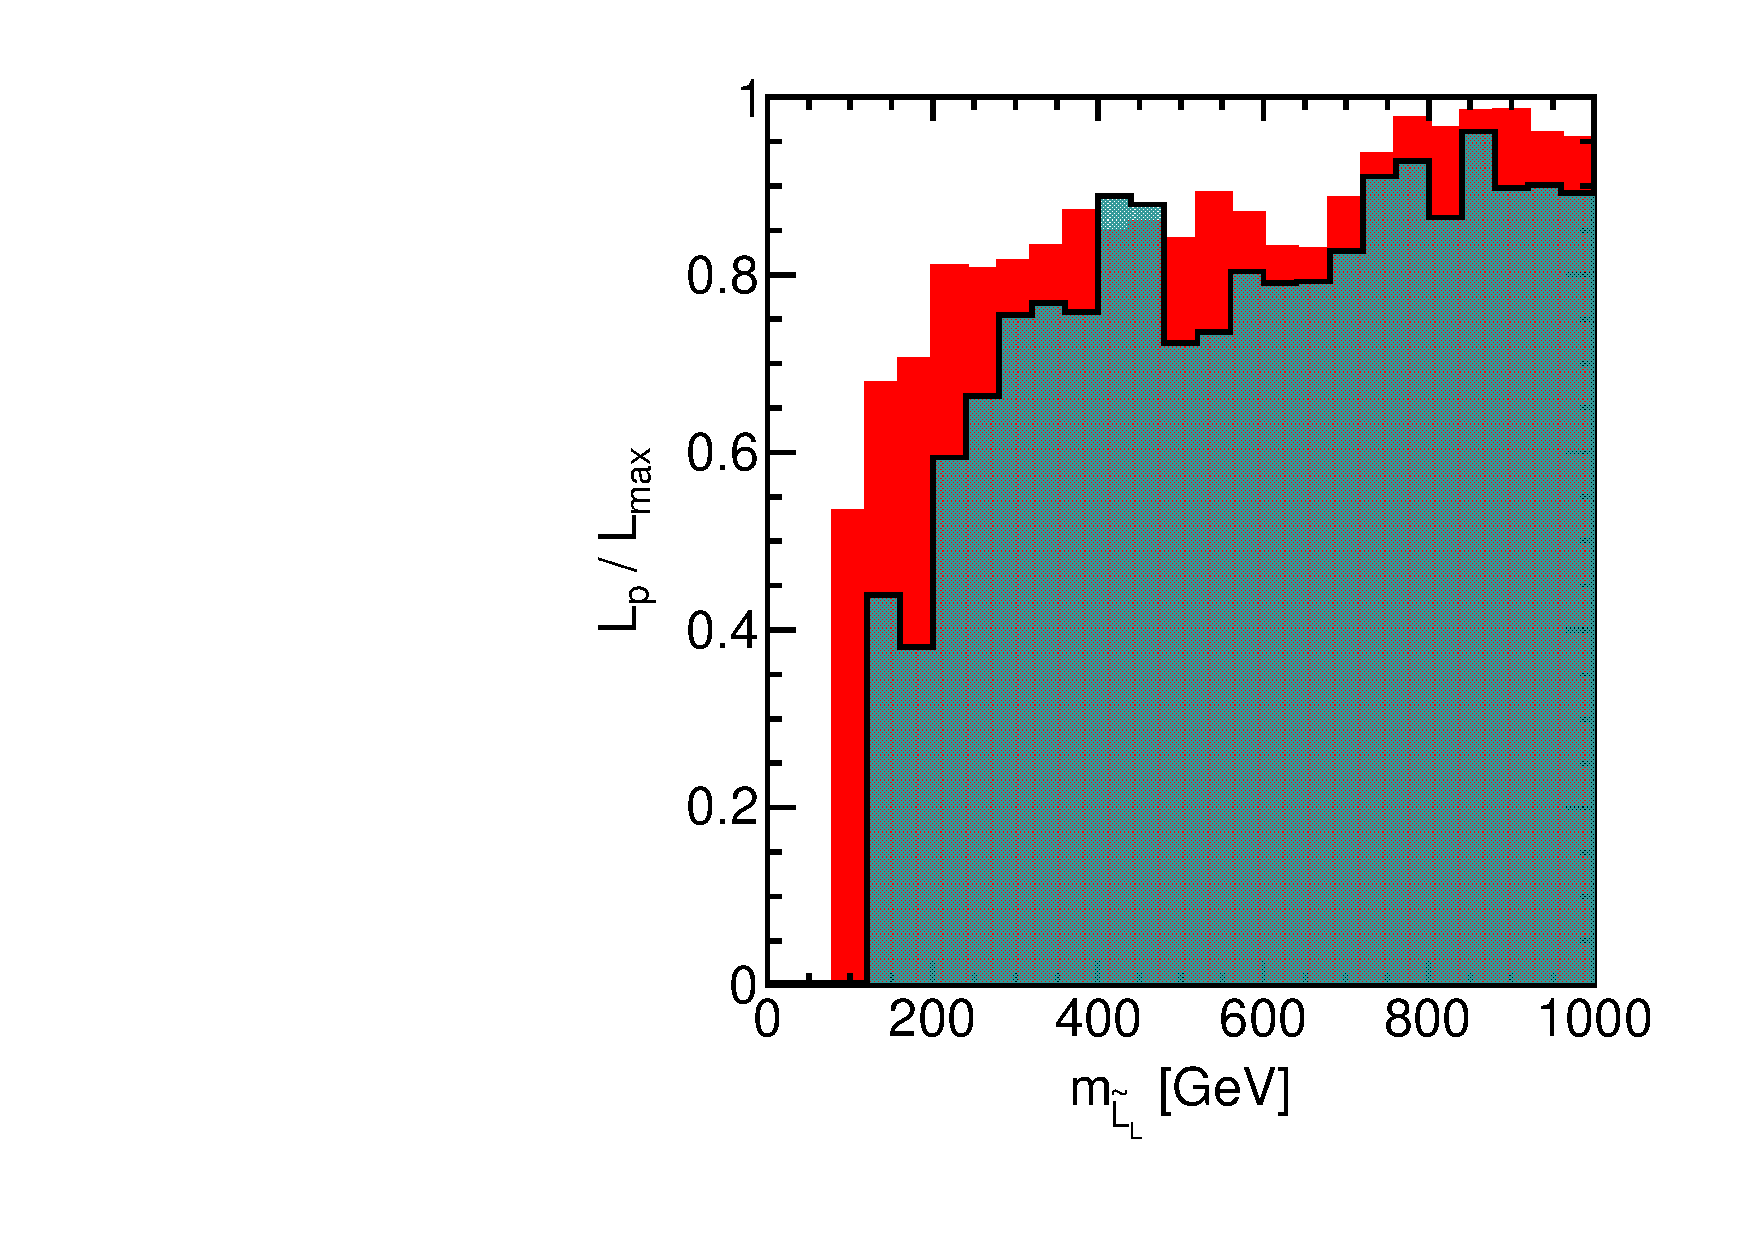
\includegraphics[height=5.5cm]{figs/fig_m_L_L.pdf} 
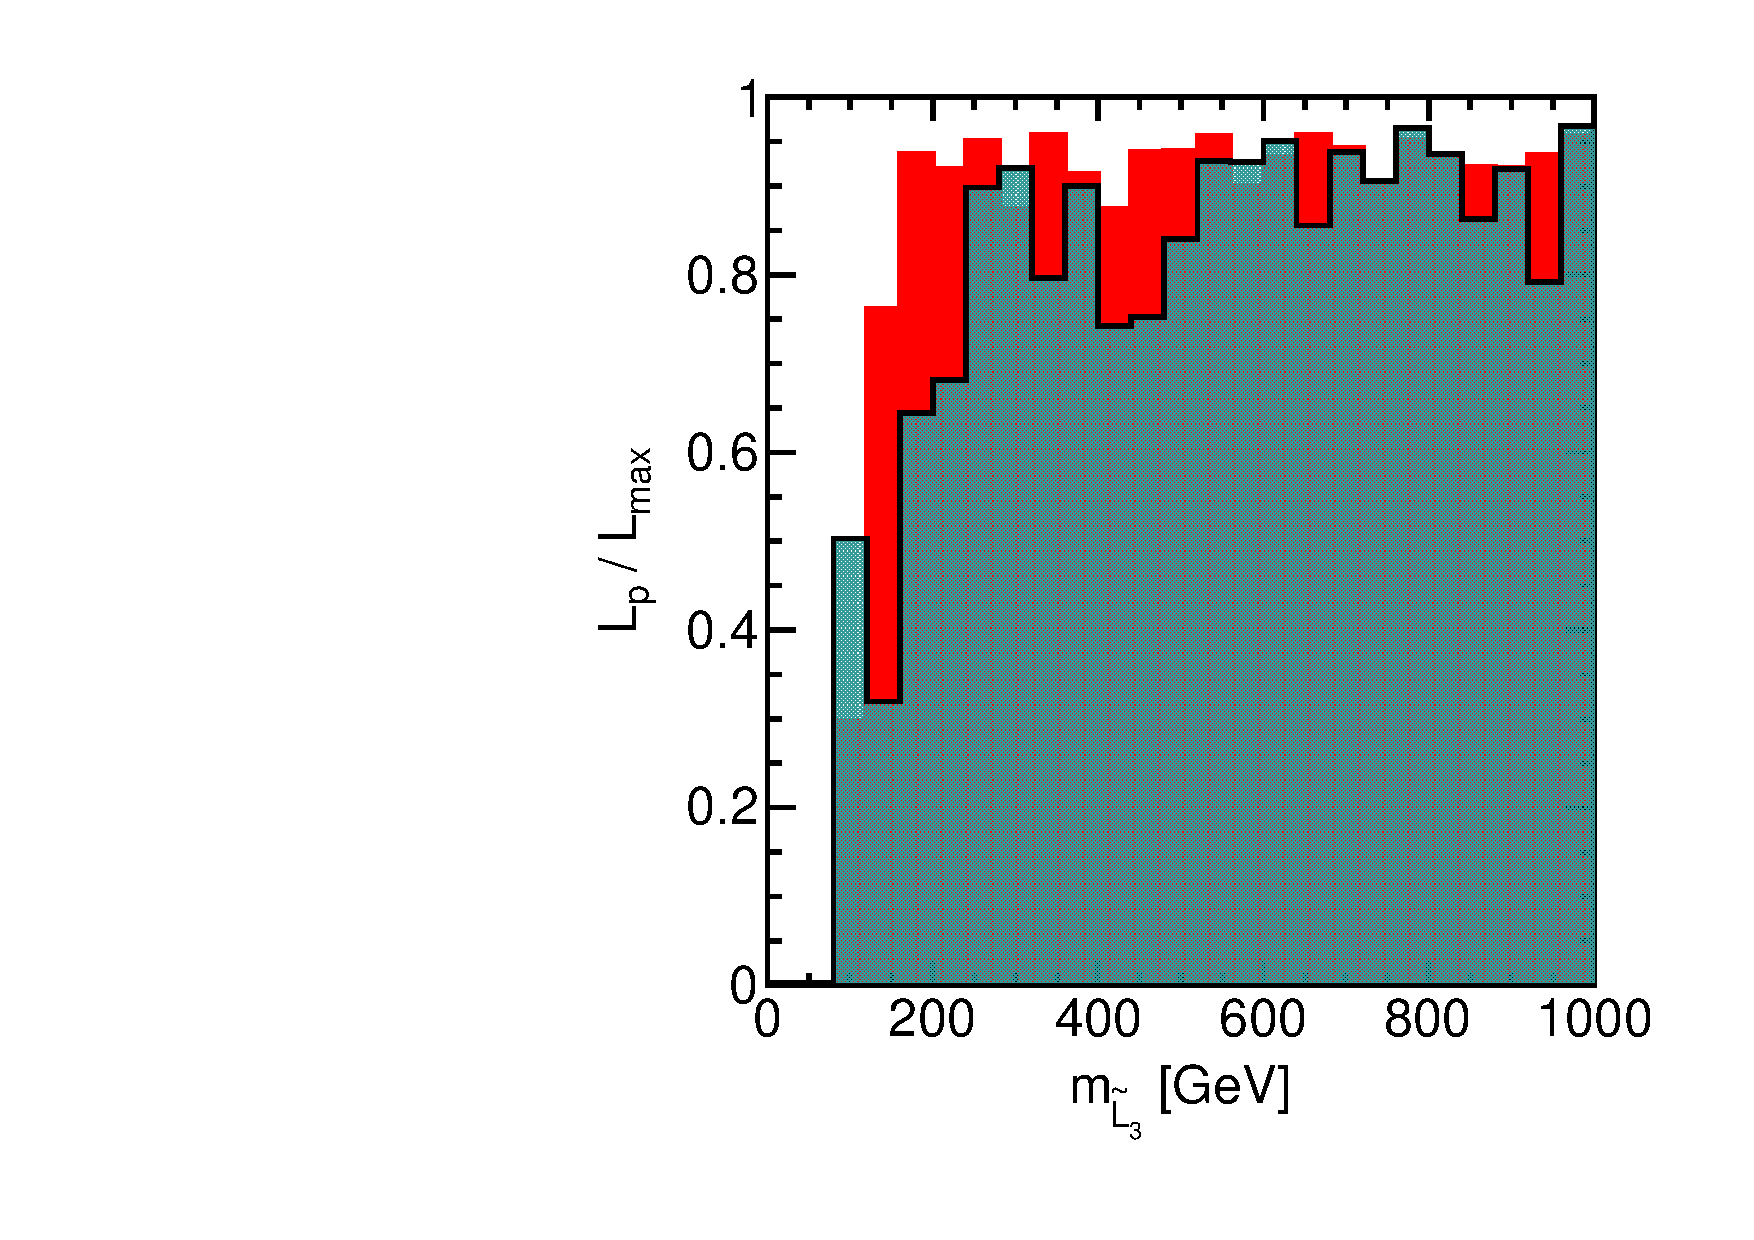
\includegraphics[height=5.5cm]{figs/fig_m_L_3.pdf} \\
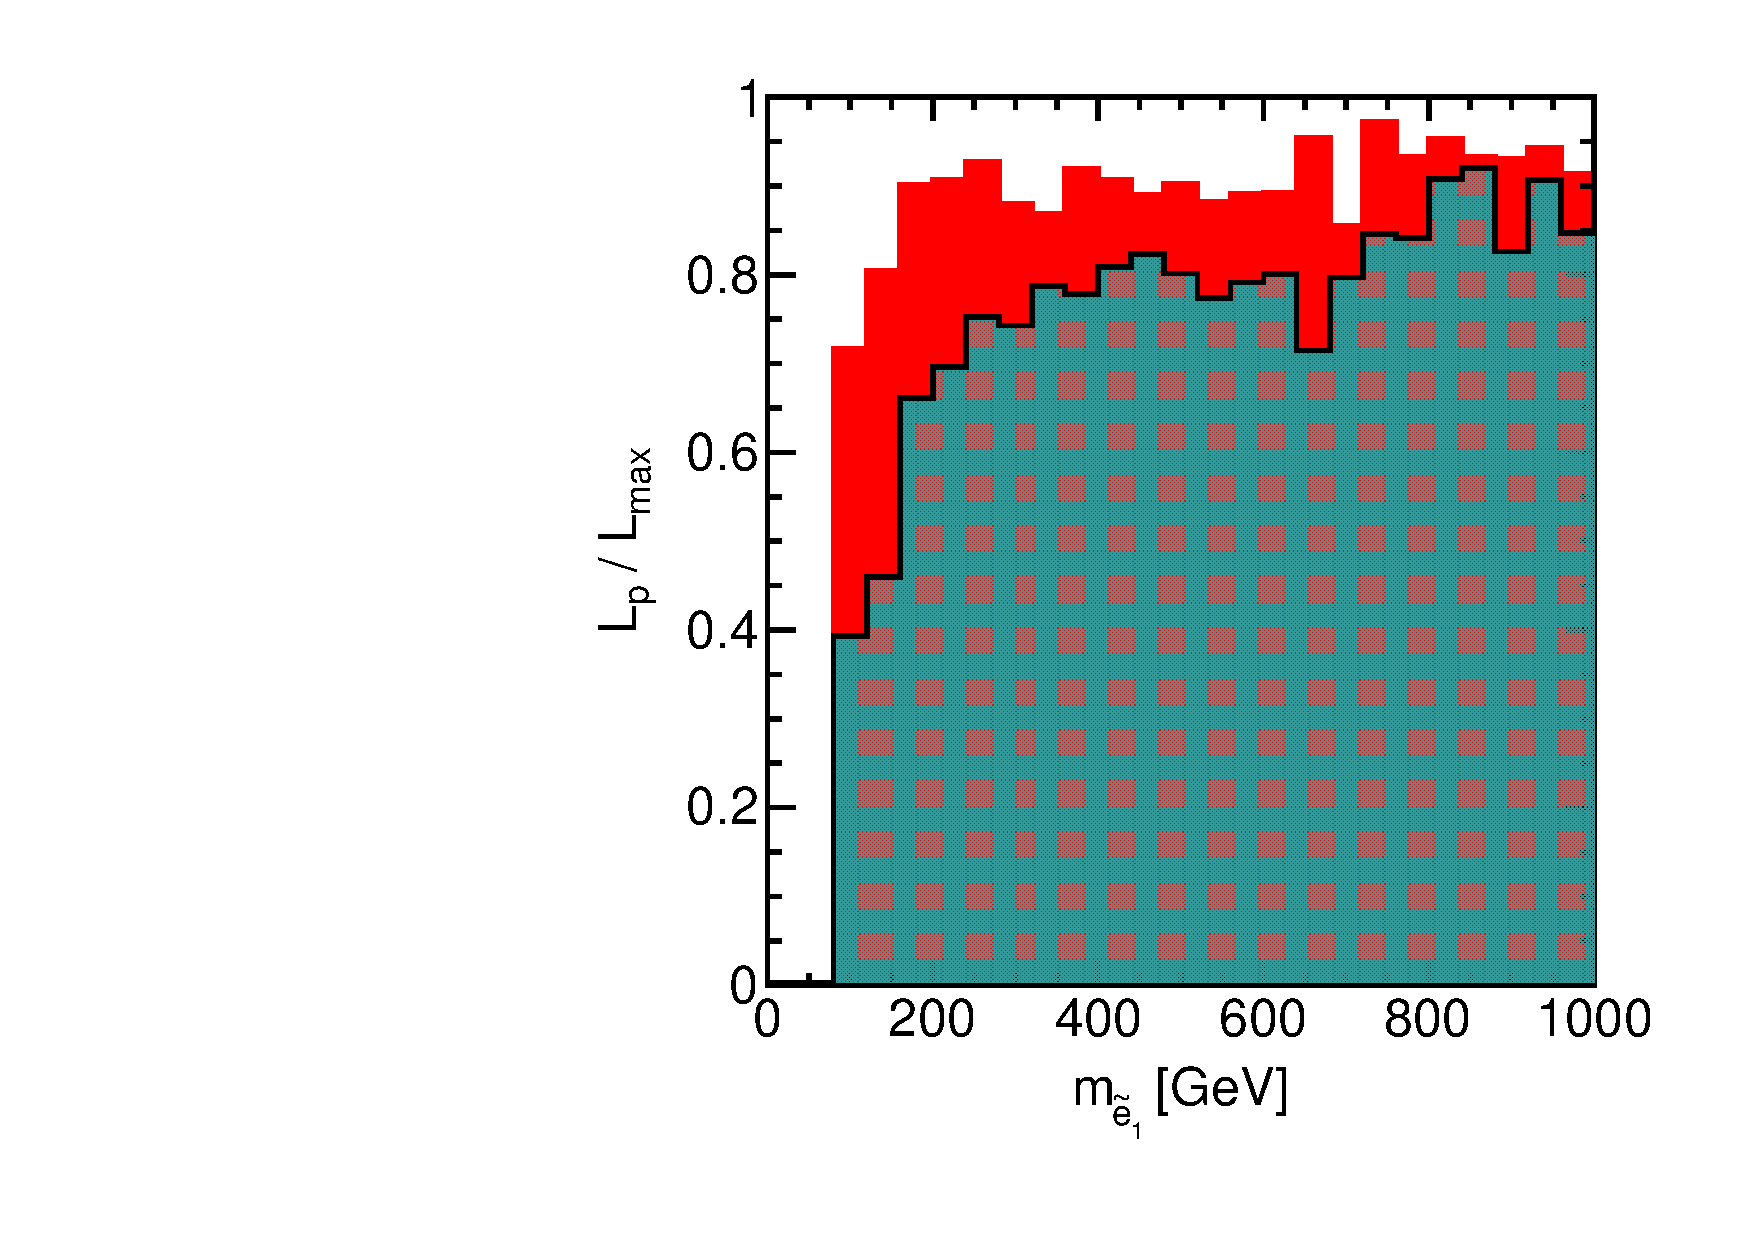
\includegraphics[height=5.5cm]{figs/fig_m_e_1.pdf}
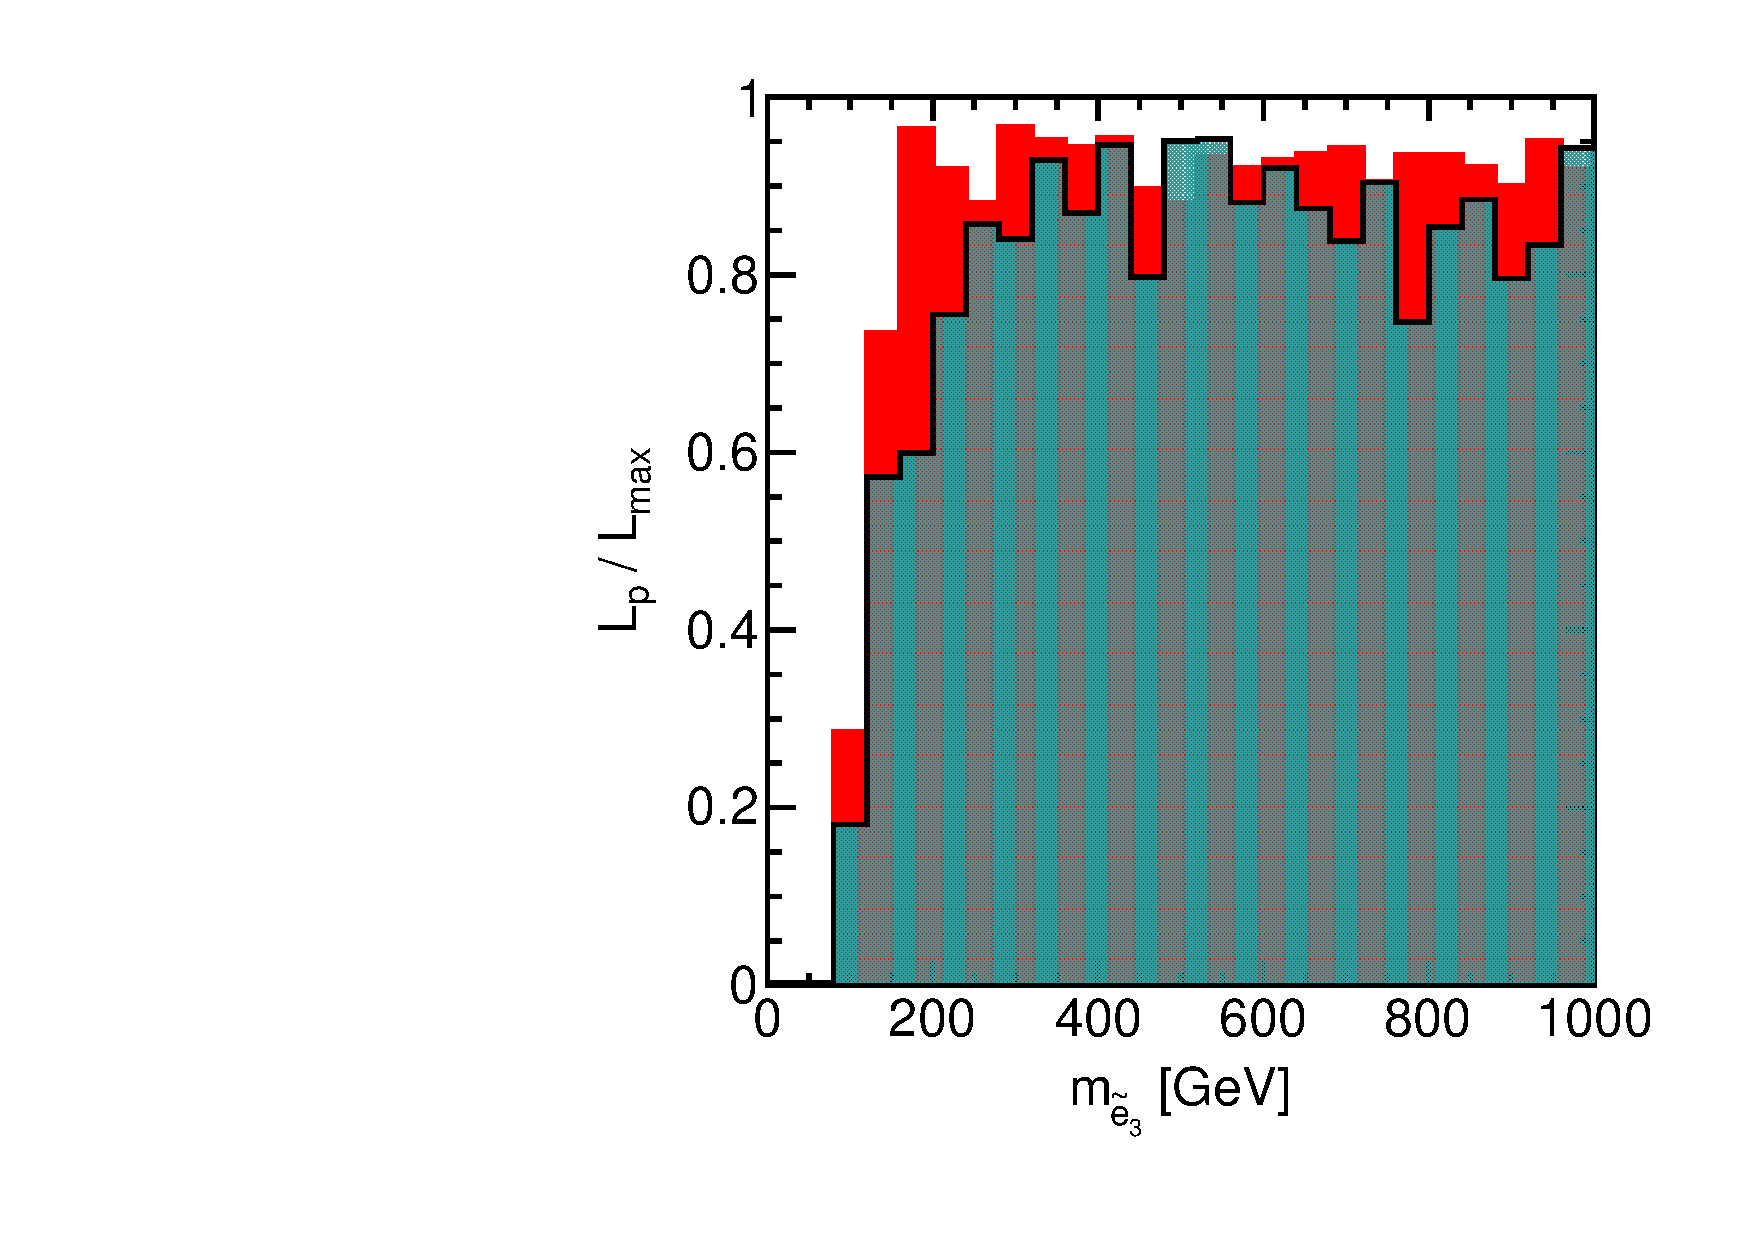
\includegraphics[height=5.5cm]{figs/fig_m_e_3.pdf}
\caption{Ratios of profile likelihood $L_p$ to maximum likelihood $L_{max}$ shown for the slepton mass parameters at SUSY scale.  The colored and shaded histograms show the distributions before and after the inclusion of the CMS results.}
\label{fig:LRwcms_msl}
\end{center}
\end{figure}


\begin{figure}[htbp]
\begin{center}
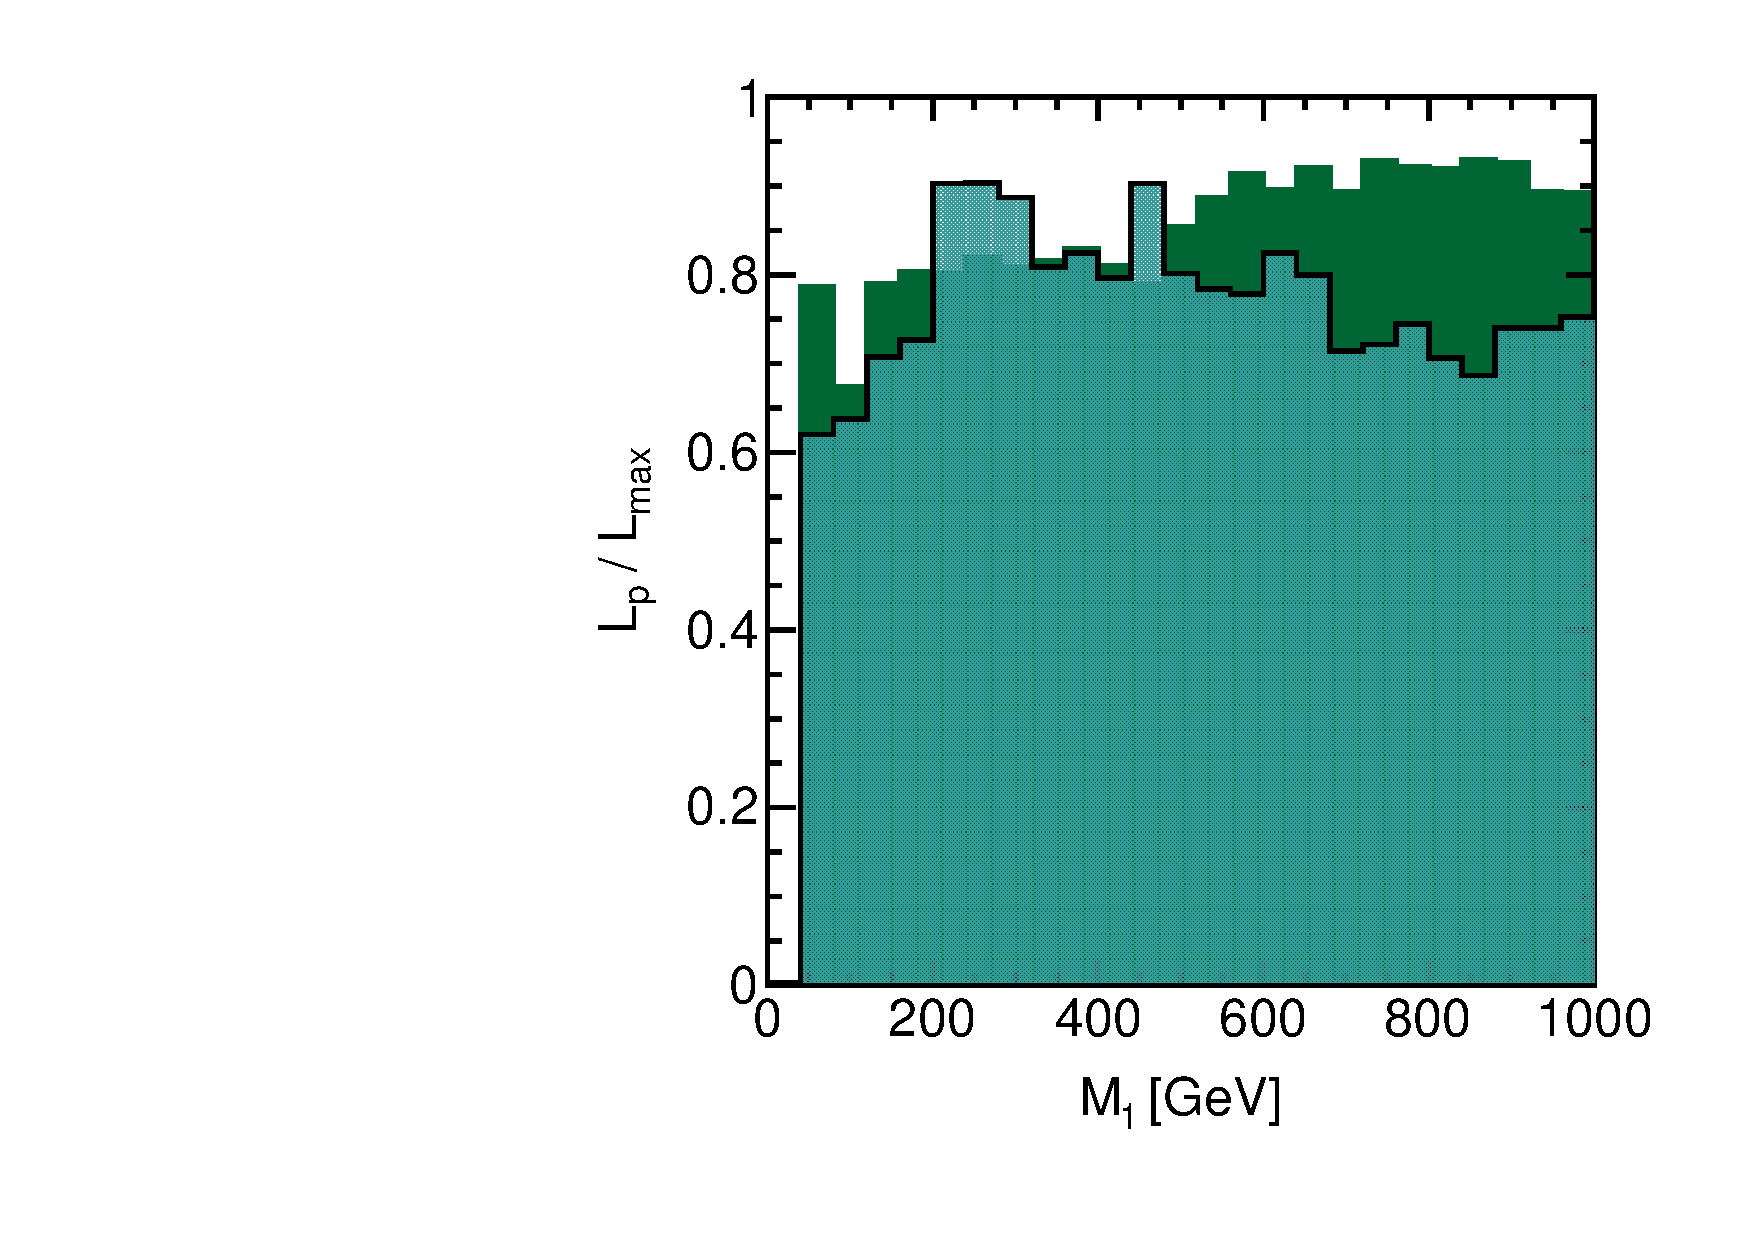
\includegraphics[height=5.5cm]{figs/fig_M_1.pdf} 
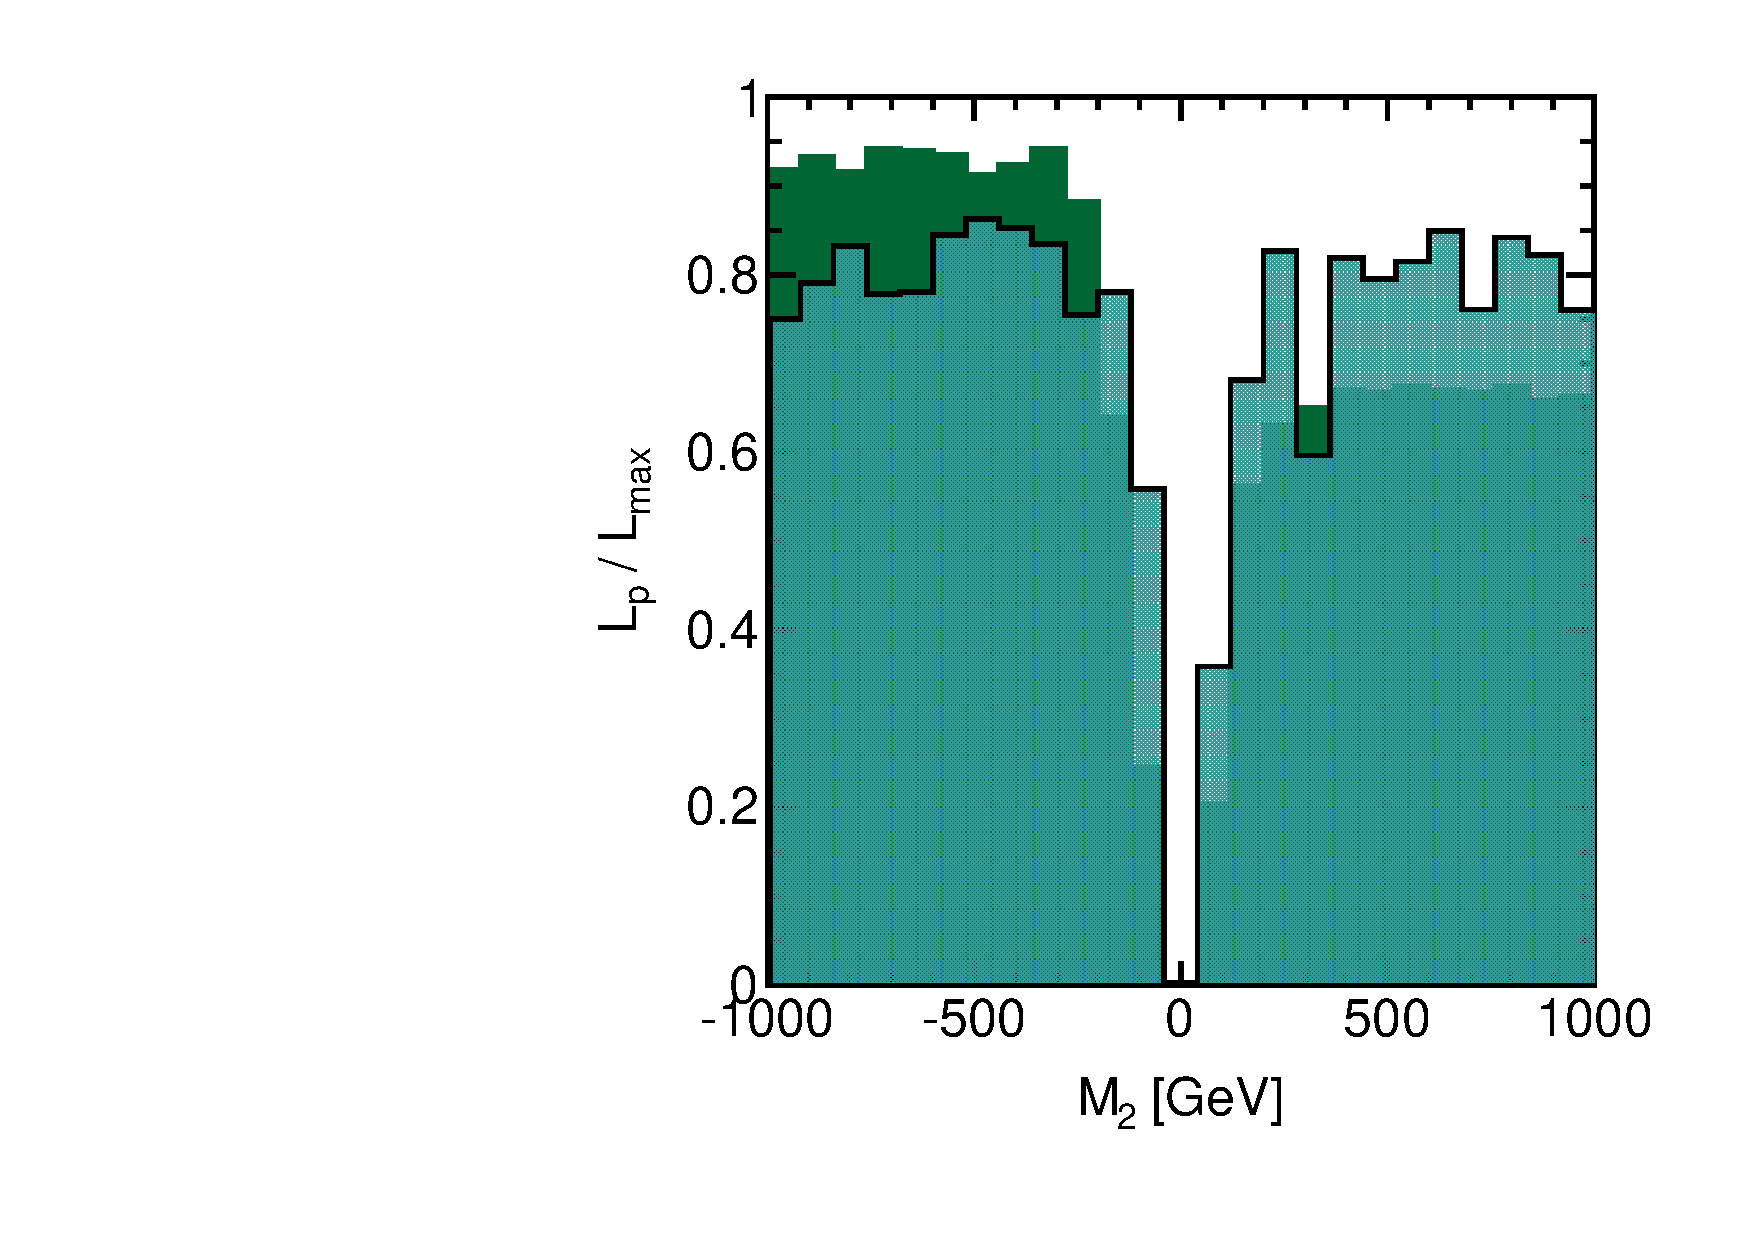
\includegraphics[height=5.5cm]{figs/fig_M_2.pdf} \\
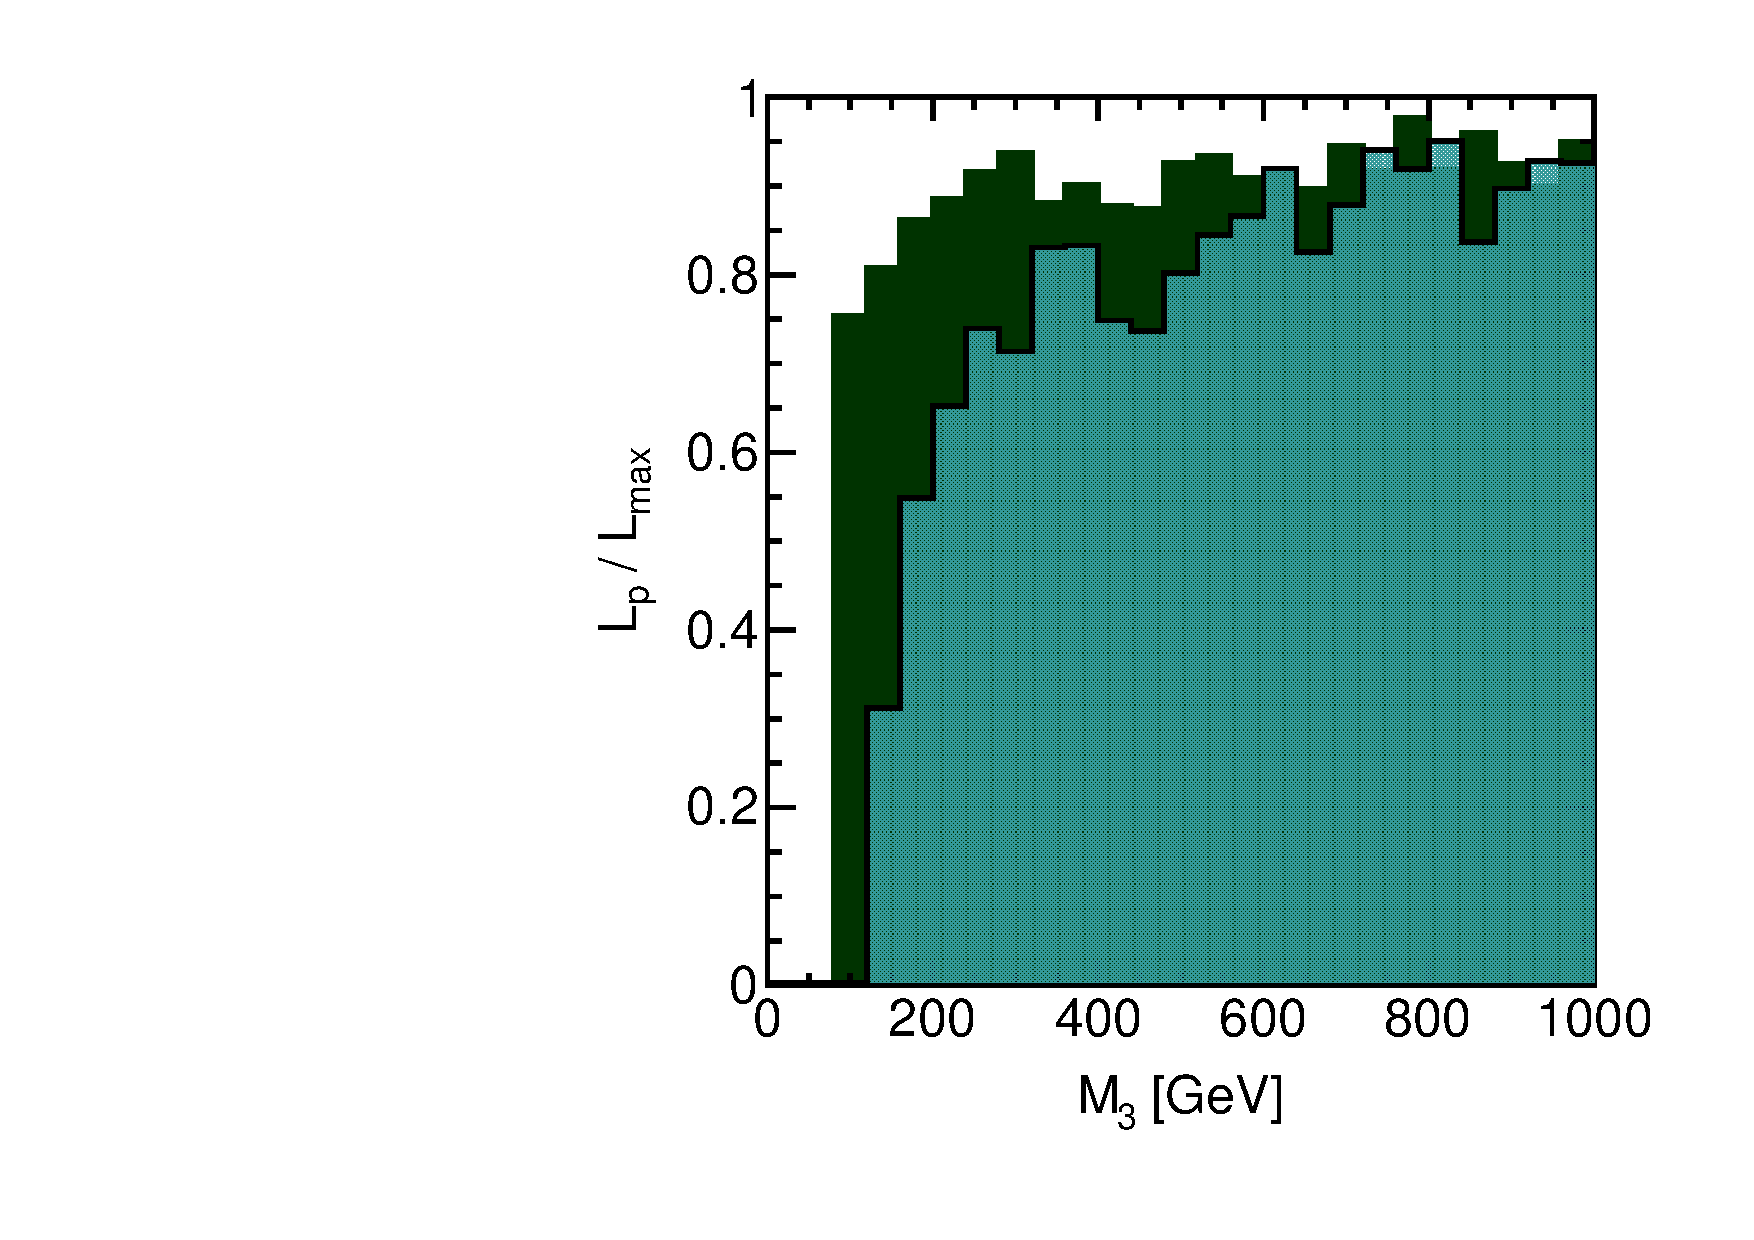
\includegraphics[height=5.5cm]{figs/fig_M_3.pdf}
\caption{Ratios of profile likelihood $L_p$ to maximum likelihood $L_{max}$ shown for gaugino mass parameters at  SUSY scale.  The colored and shaded histograms show the distributions before and after the inclusion of the CMS results.}
\label{fig:LRwcms_M}
\end{center}
\end{figure}


\begin{figure}[htbp]
\begin{center}
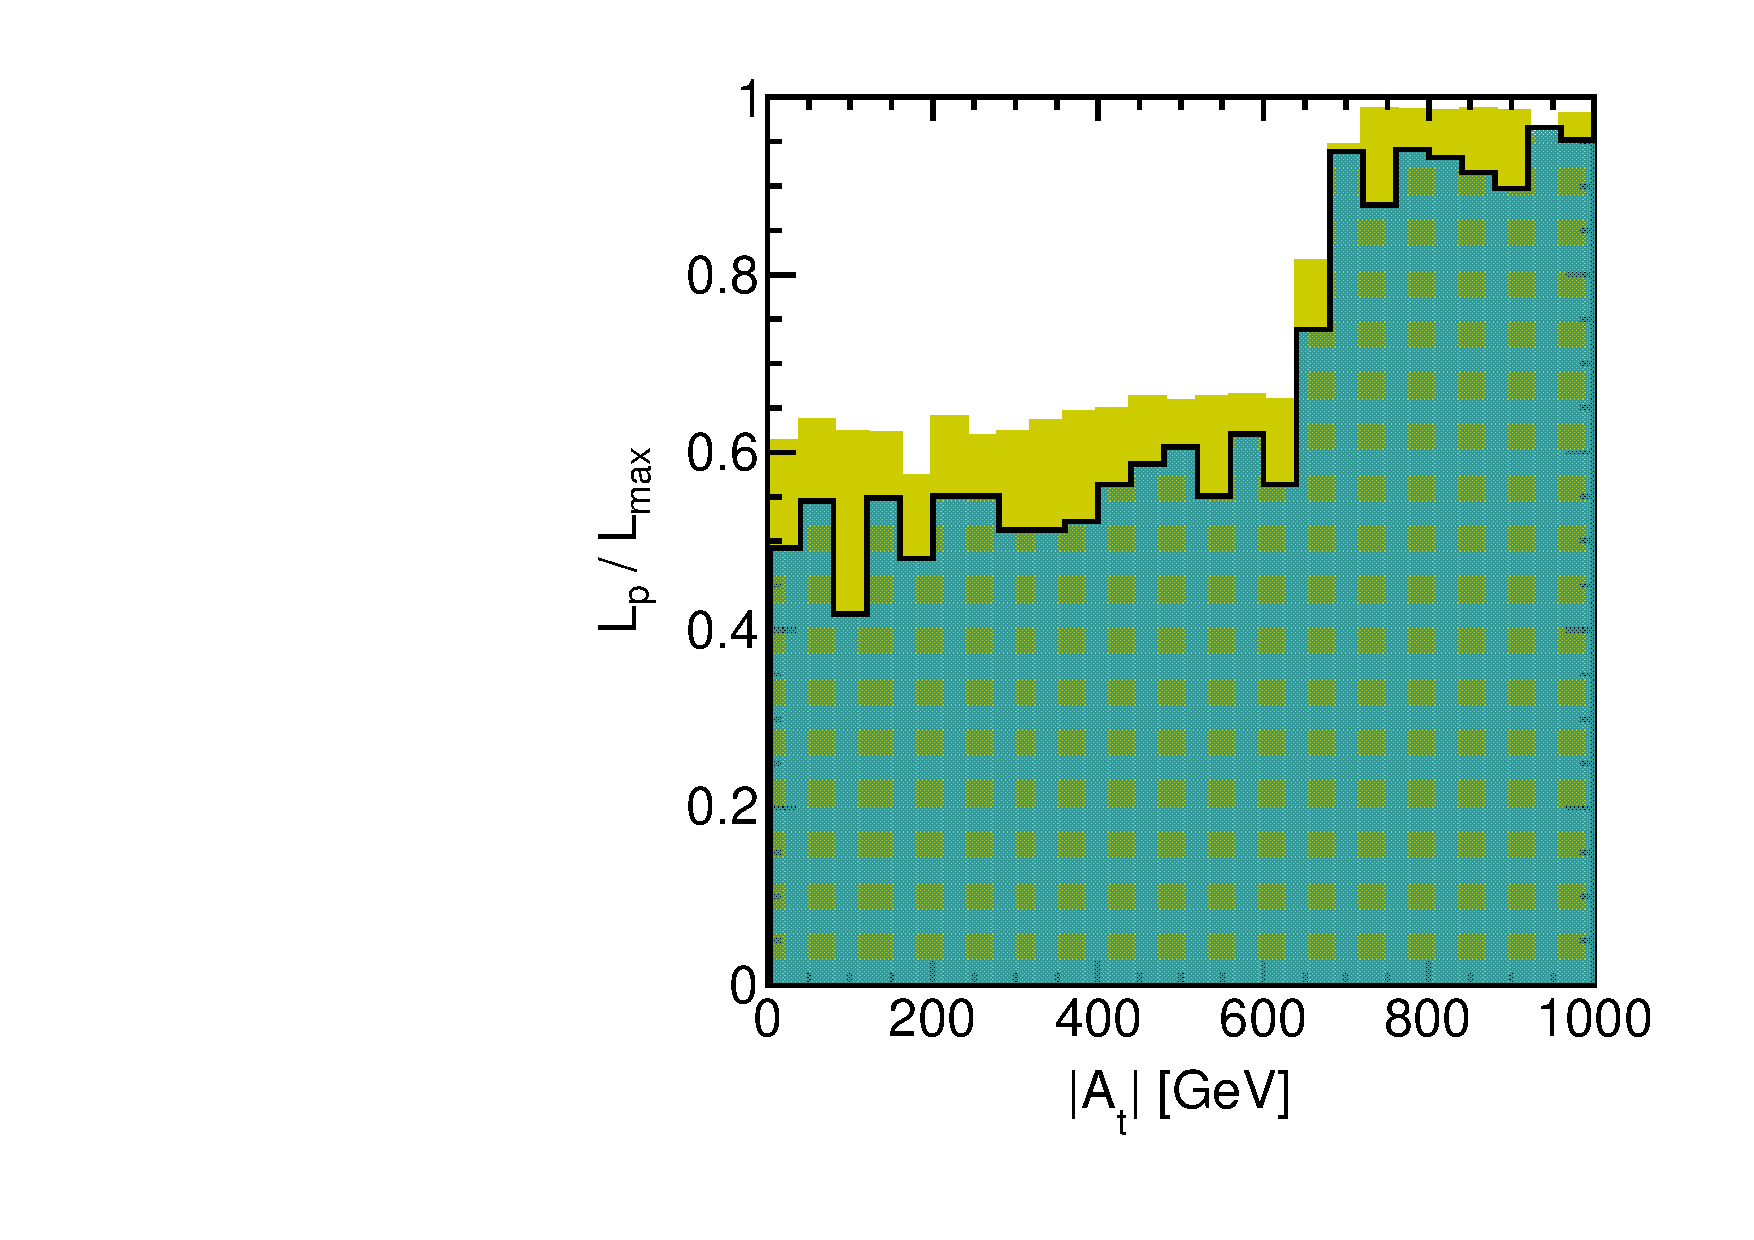
\includegraphics[height=5.5cm]{figs/fig_A_t.pdf} 
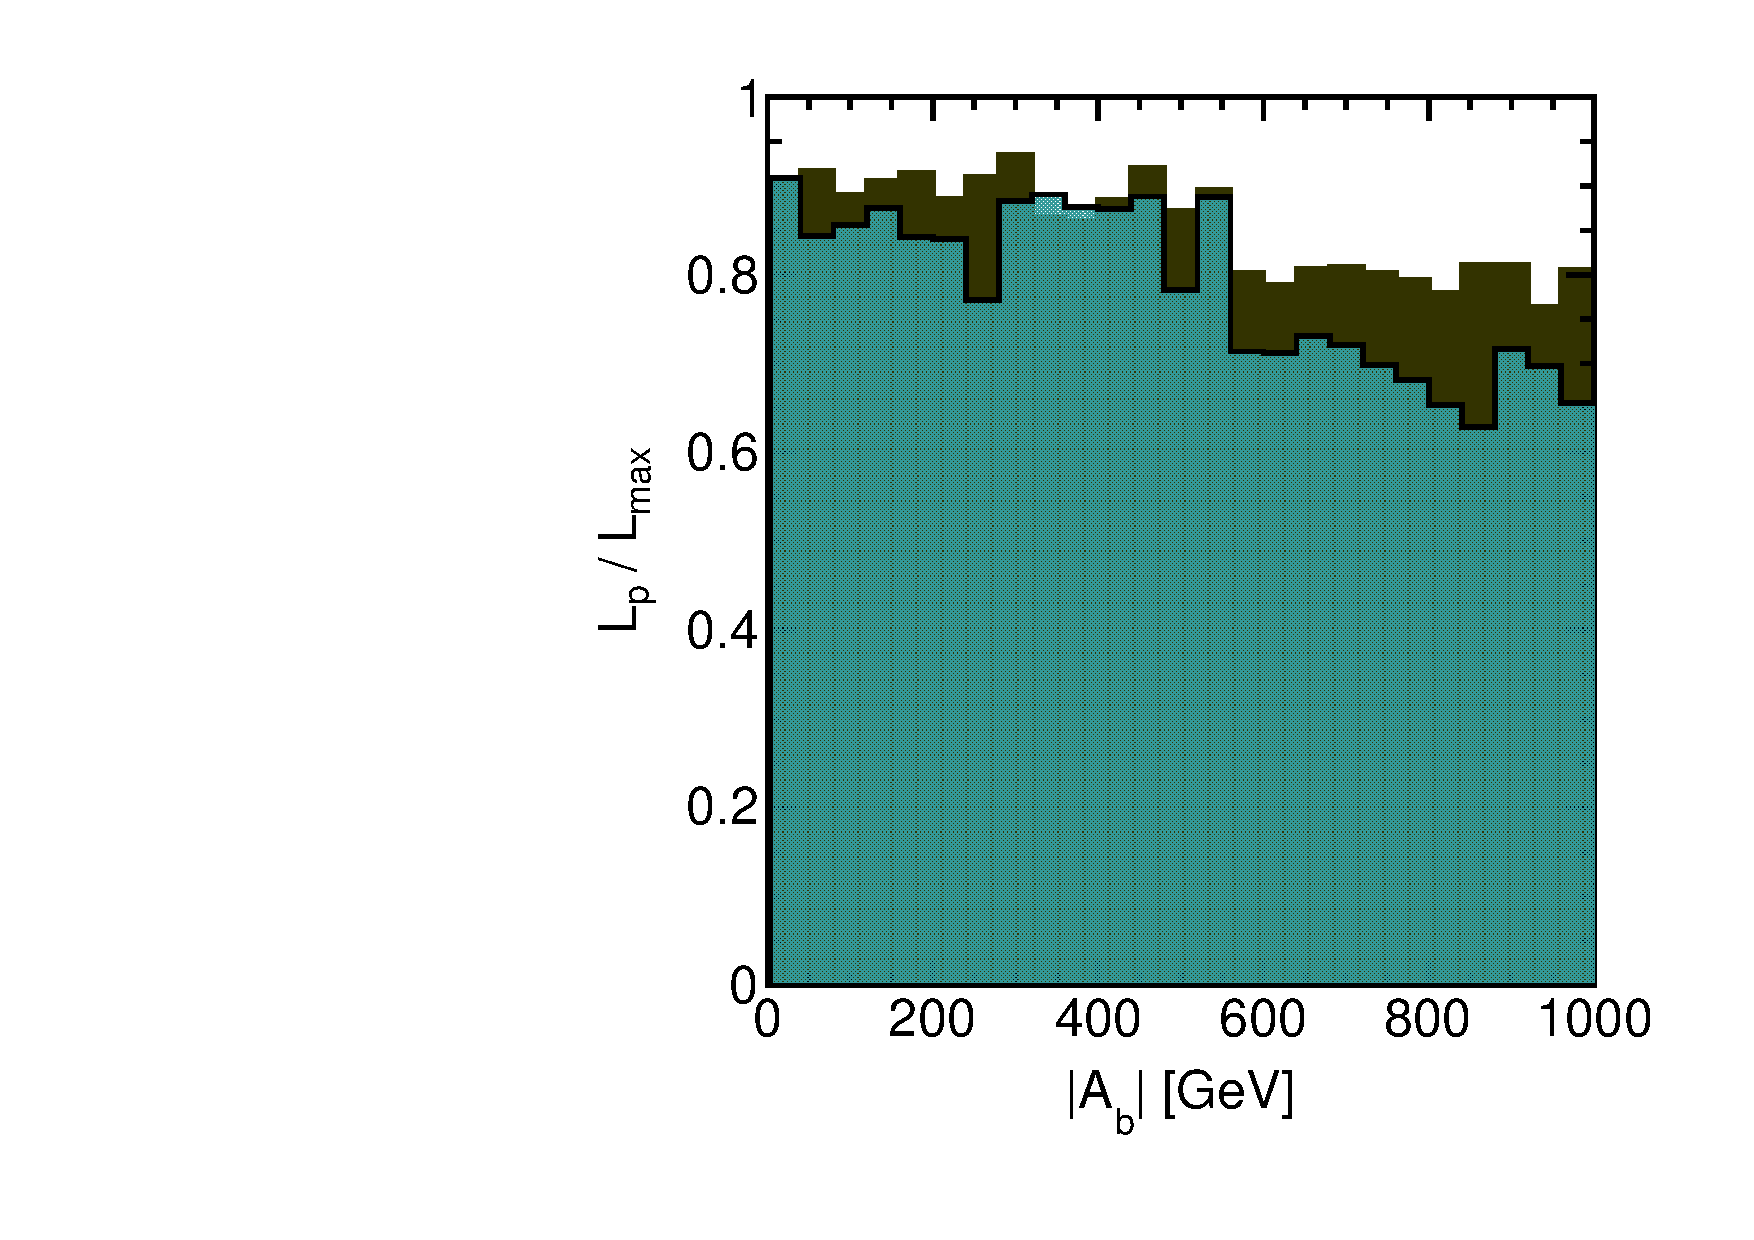
\includegraphics[height=5.5cm]{figs/fig_A_b.pdf} \\
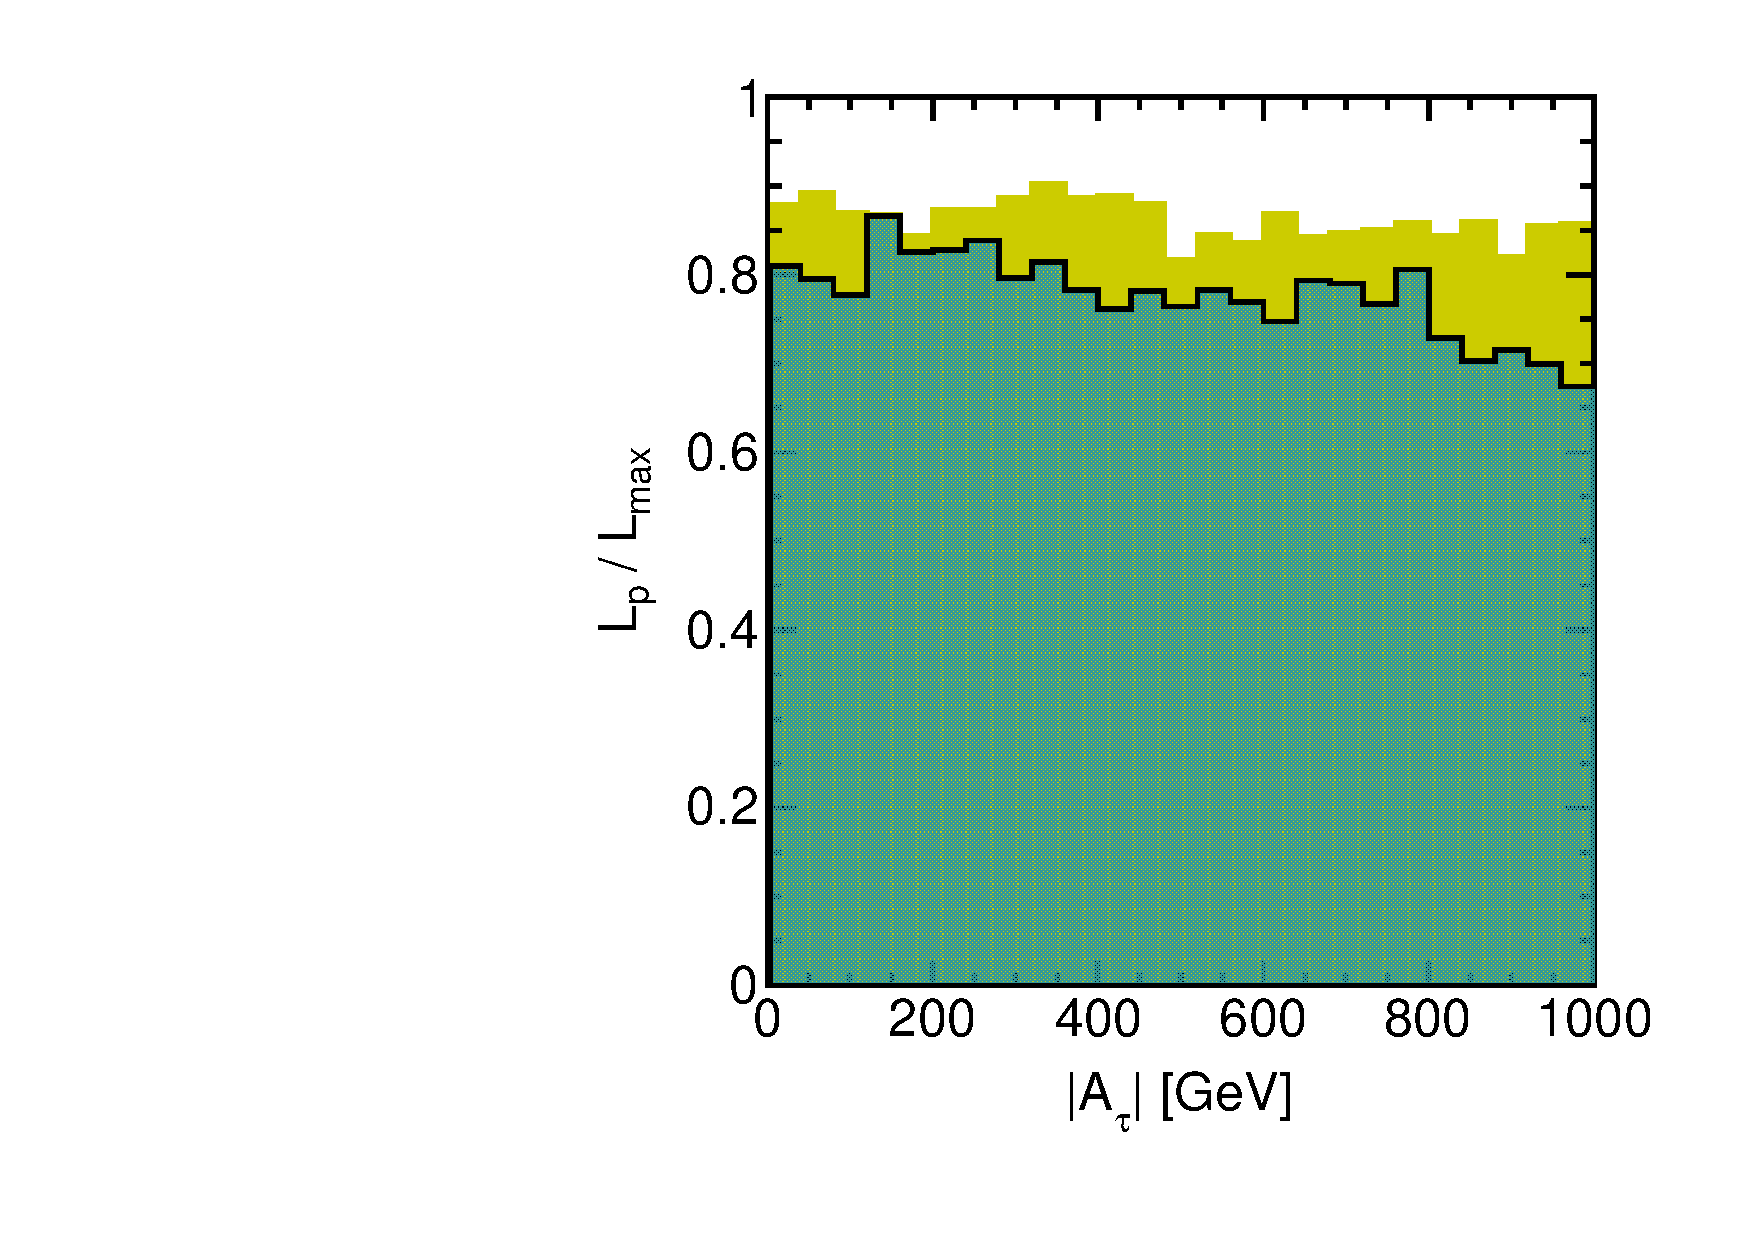
\includegraphics[height=5.5cm]{figs/fig_A_tau.pdf}
\caption{Ratios of profile likelihood $L_p$ to maximum likelihood $L_{max}$ shown for trilinear couplings at SUSY scale.  The colored and shaded histograms show the distributions before and after the inclusion of the CMS results.}
\label{fig:LRwcms_A}
\end{center}
\end{figure}

\begin{figure}[htbp]
\begin{center}
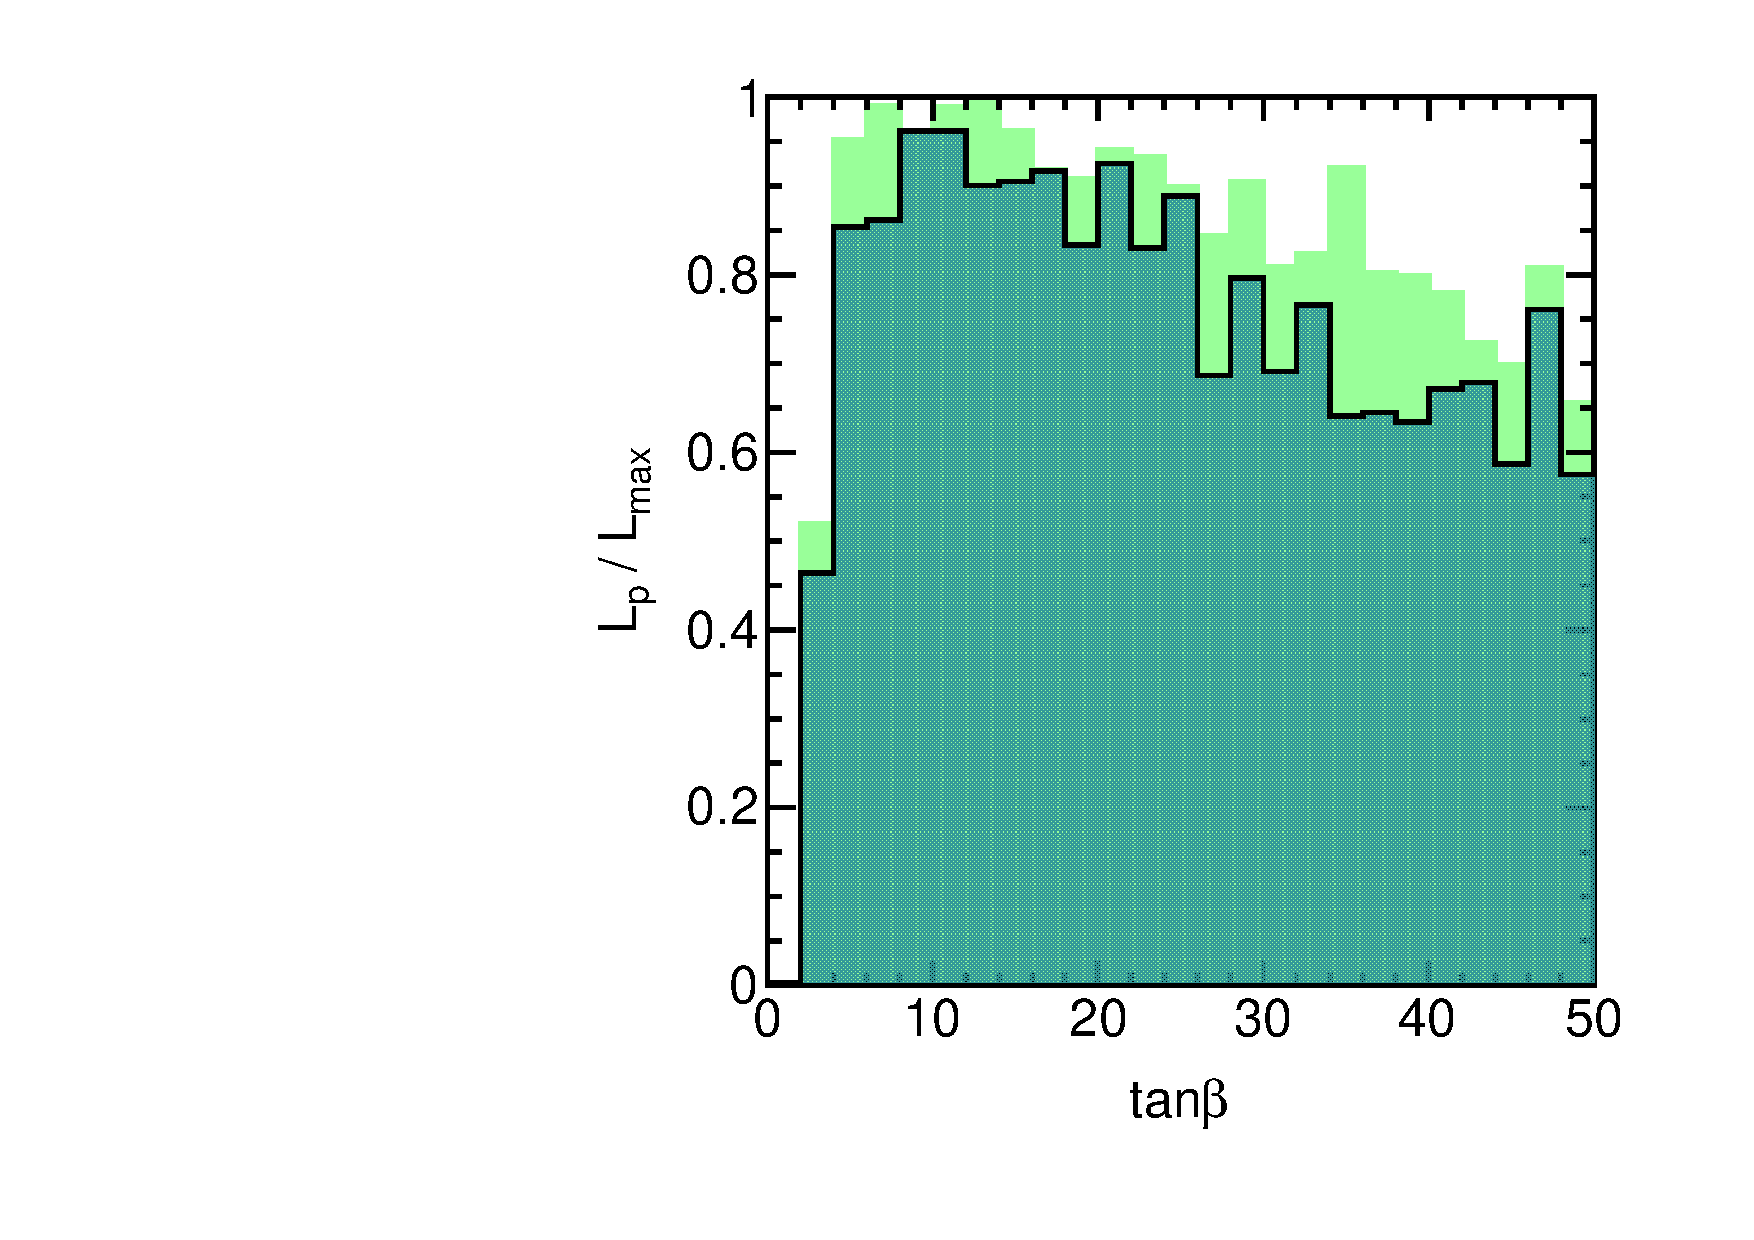
\includegraphics[height=5.5cm]{figs/fig_tanbeta.pdf} 
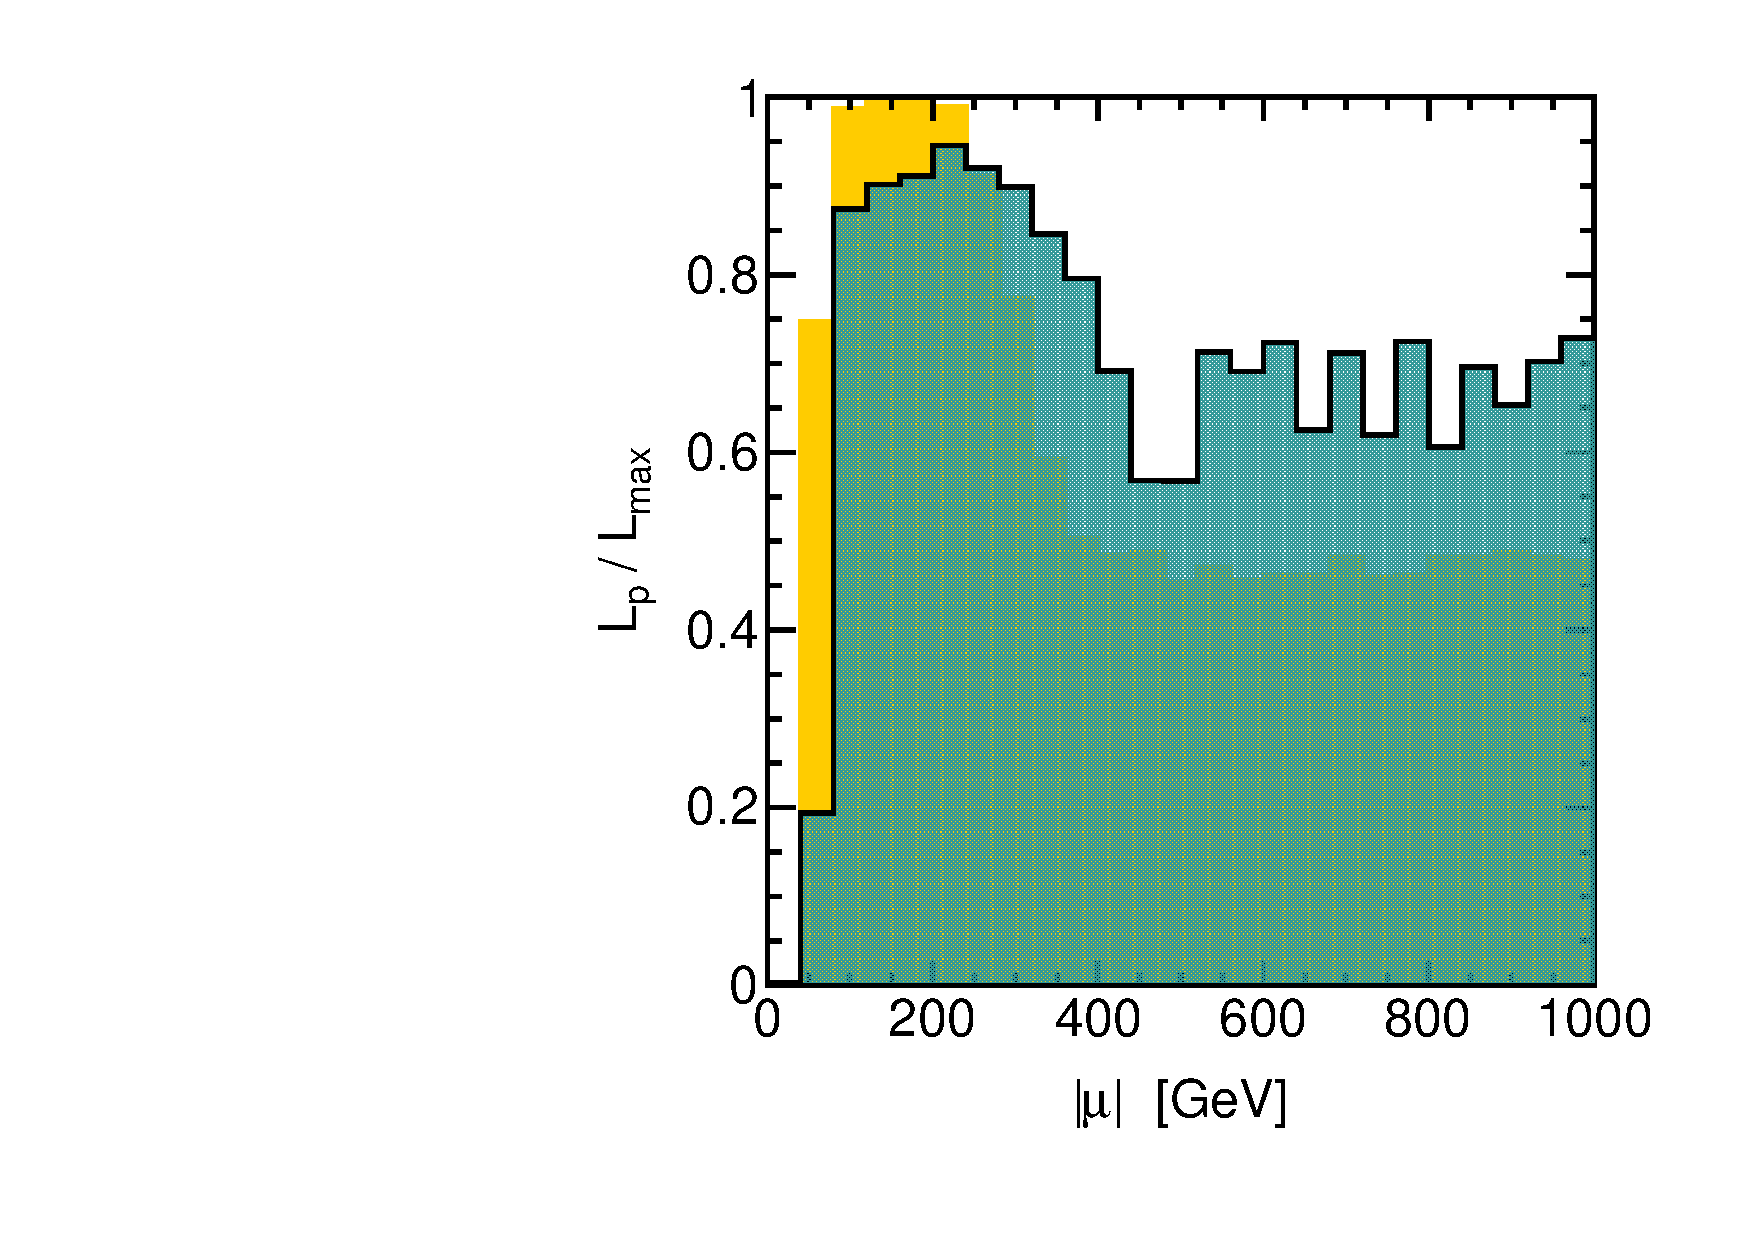
\includegraphics[height=5.5cm]{figs/fig_mu.pdf} 
\caption{Ratios of profile likelihood $L_p$ to maximum likelihood $L_{max}$ shown for $\tan\beta$ and $\mu$ parameter at SUSY scale.  The colored and shaded histograms show the distributions before and after the inclusion of the CMS results.}
\label{fig:LRwcms_tbmu}
\end{center}
\end{figure}



\begin{figure}[htbp]
\begin{center}
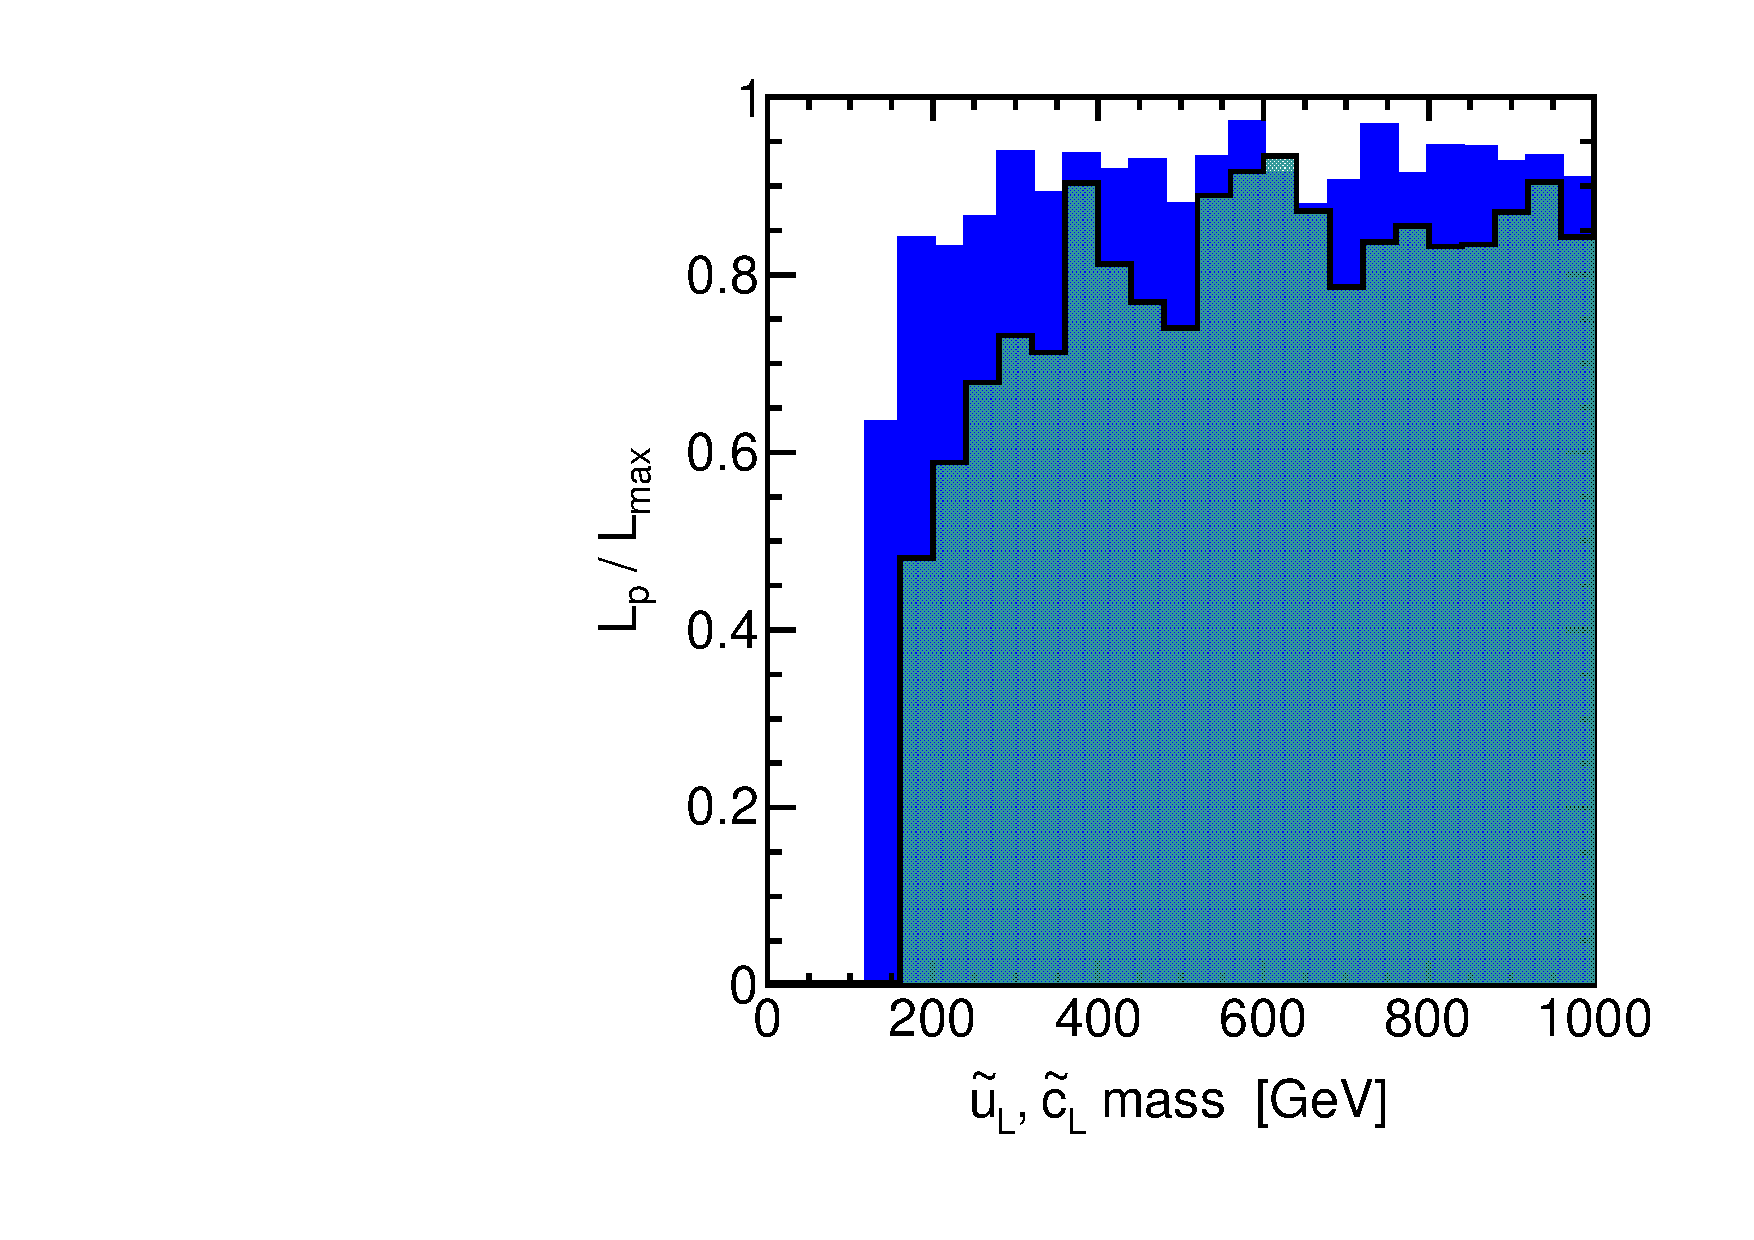
\includegraphics[height=5.5cm]{figs/fig_u_L.pdf} 
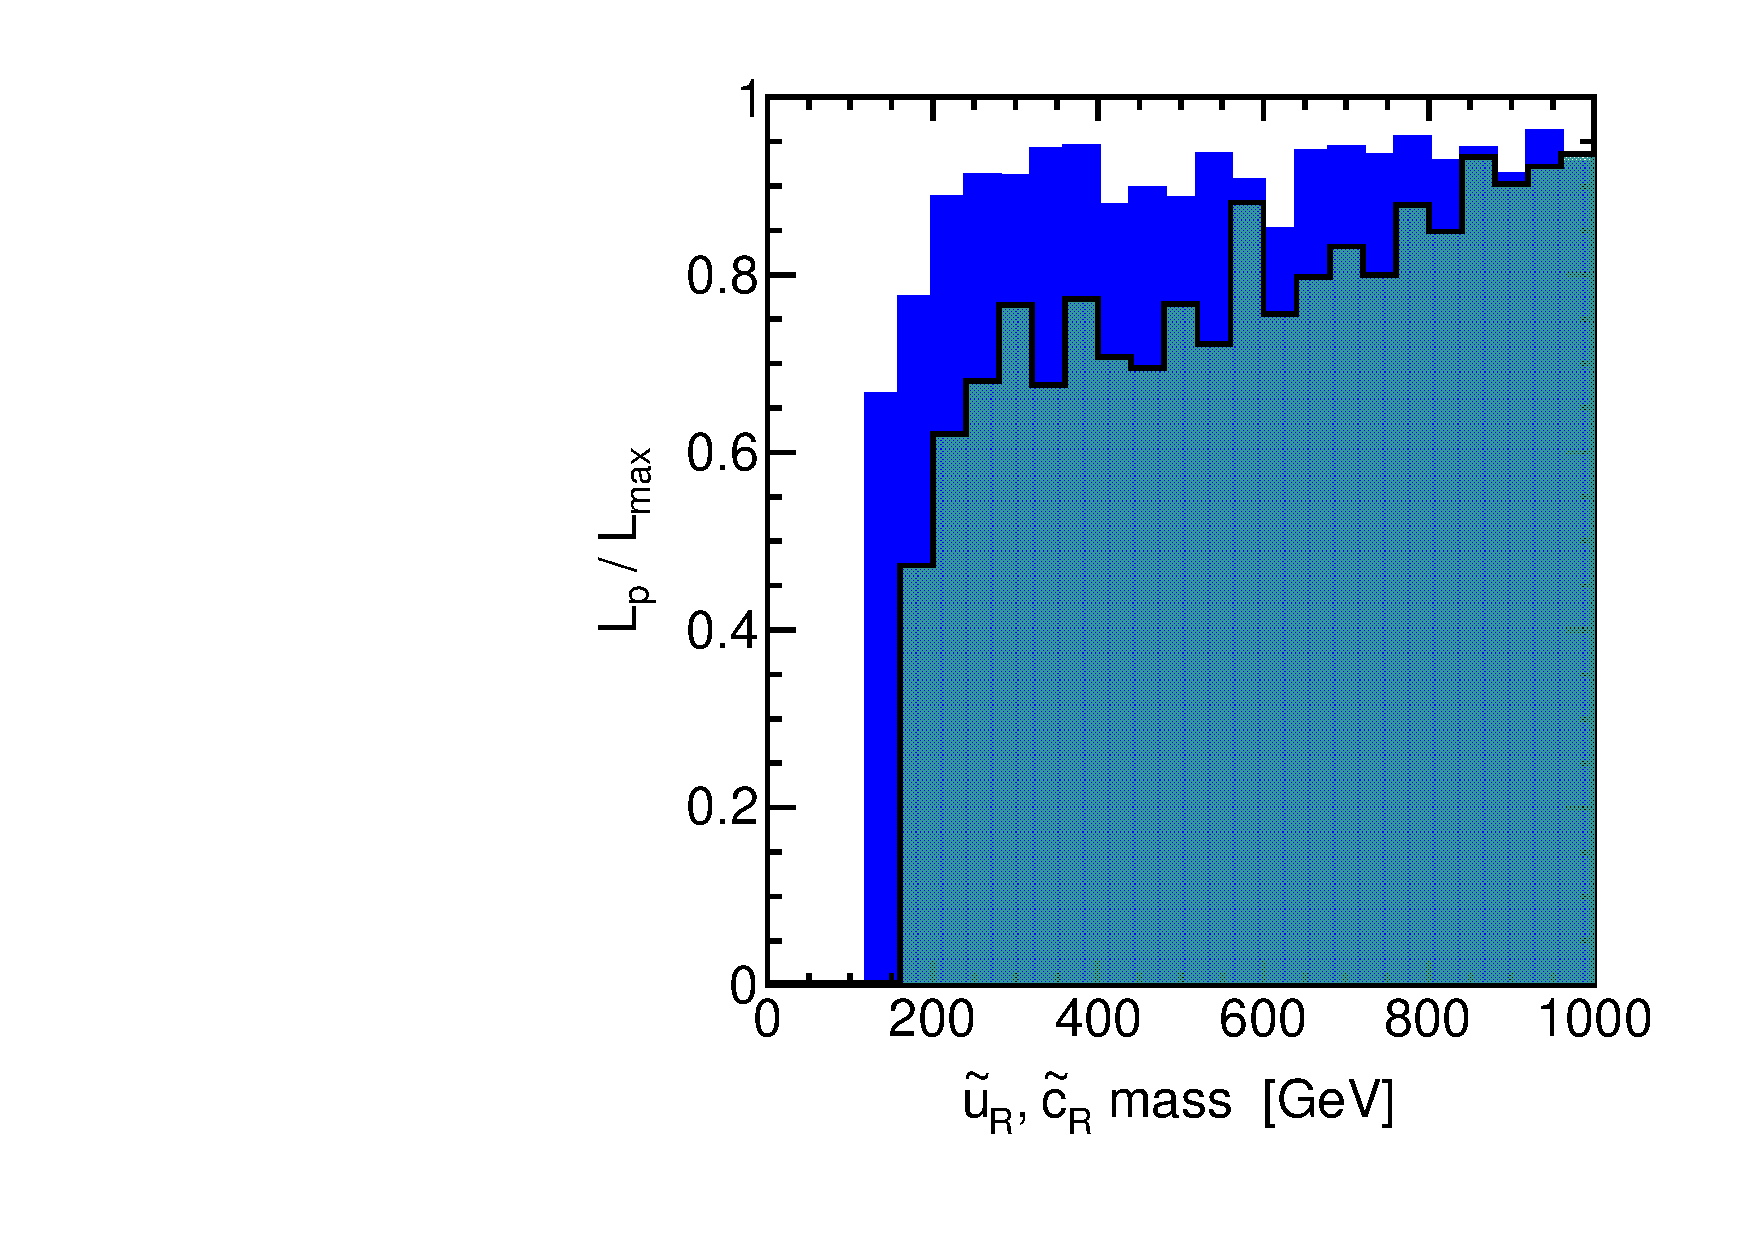
\includegraphics[height=5.5cm]{figs/fig_u_R.pdf} \\
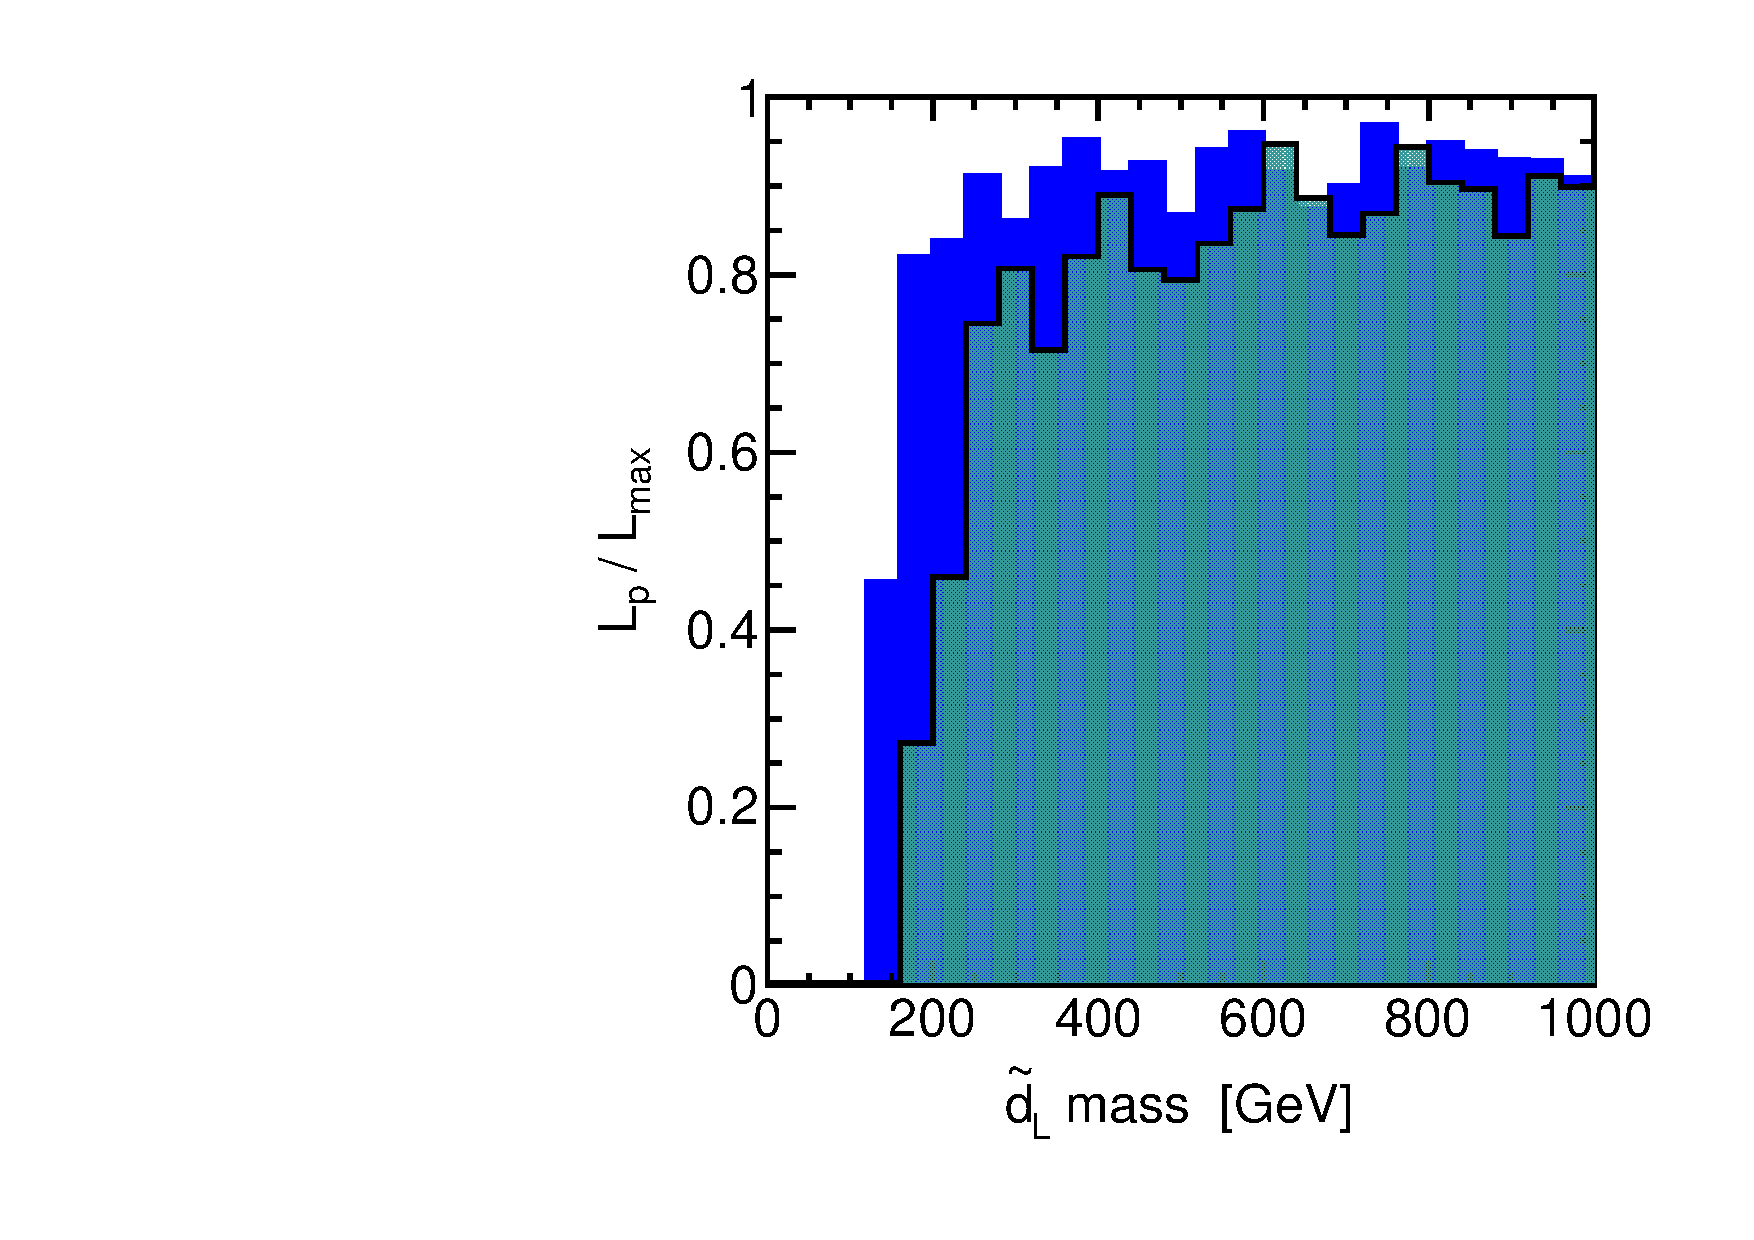
\includegraphics[height=5.5cm]{figs/fig_d_L.pdf} 
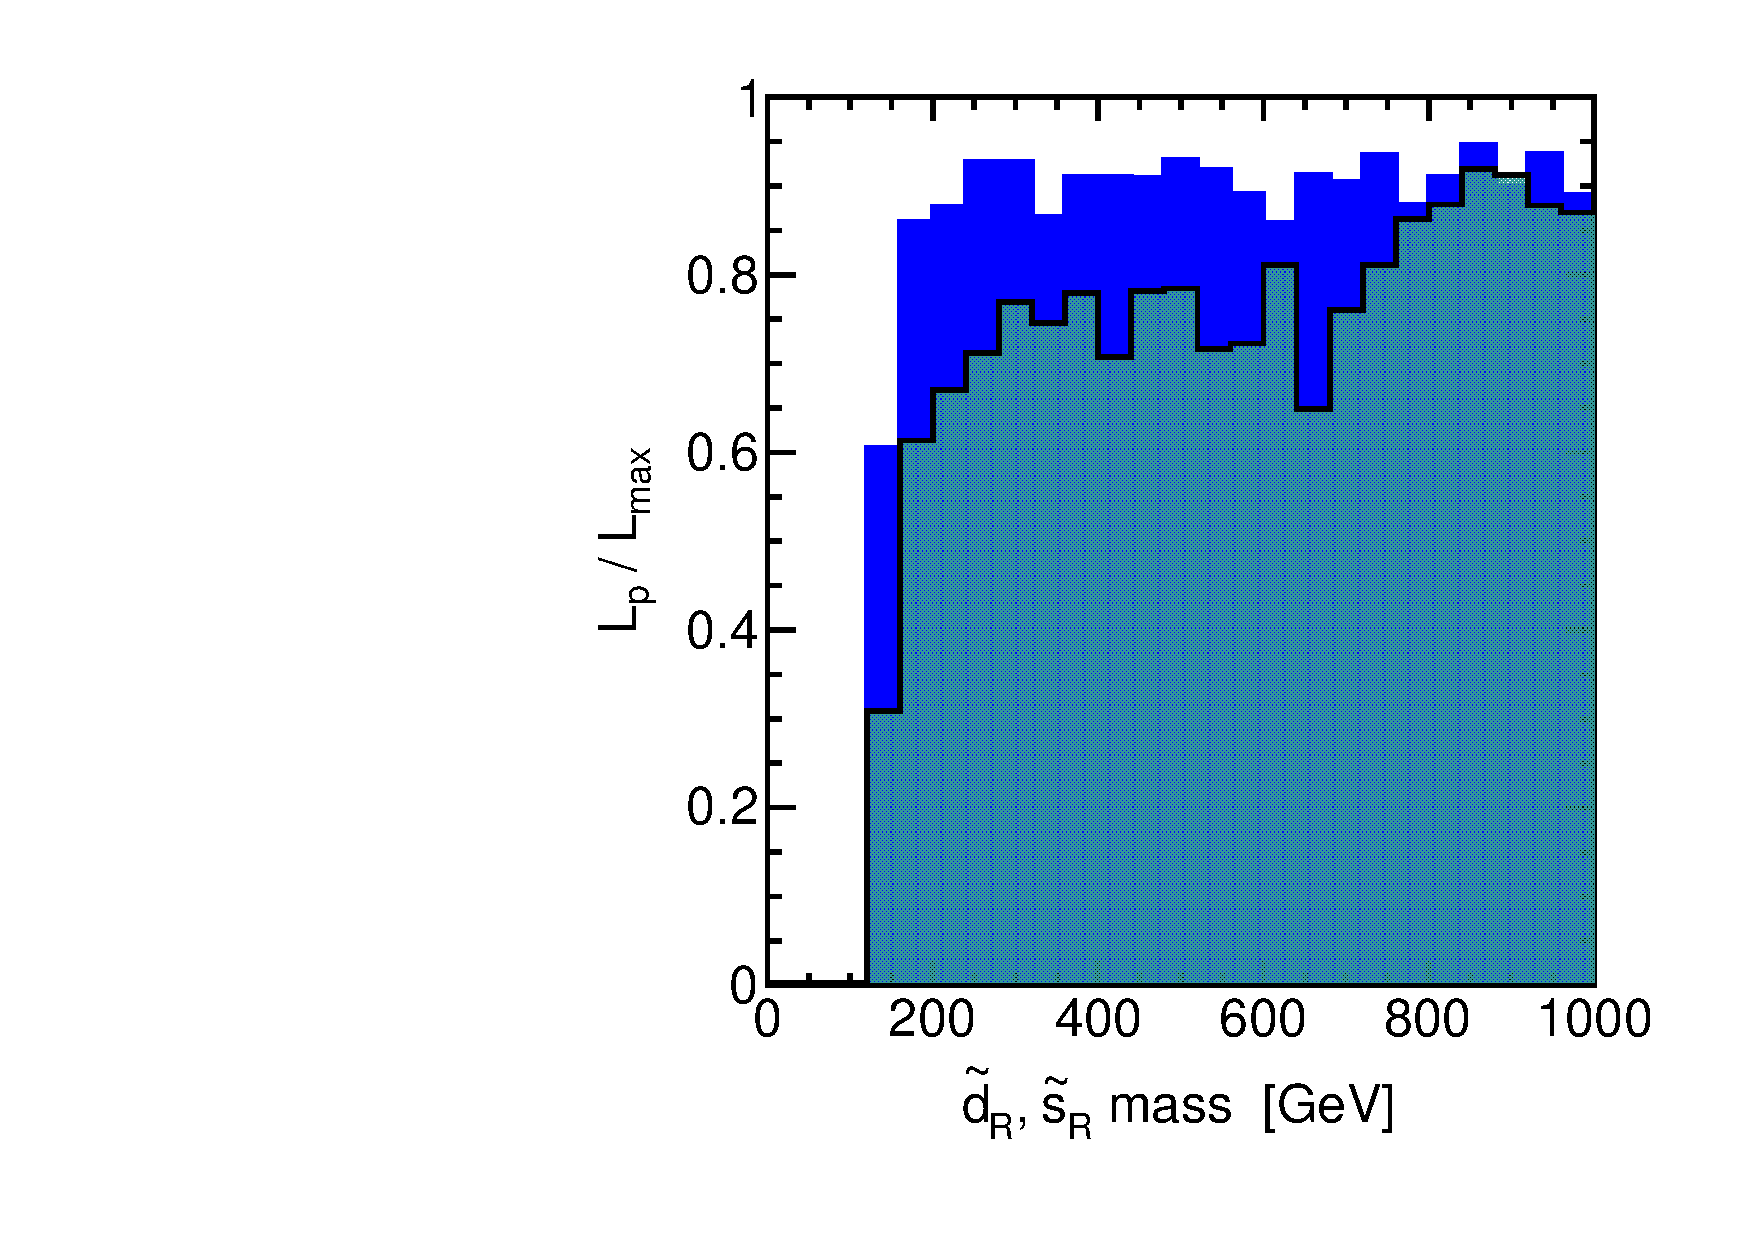
\includegraphics[height=5.5cm]{figs/fig_d_R.pdf} \\
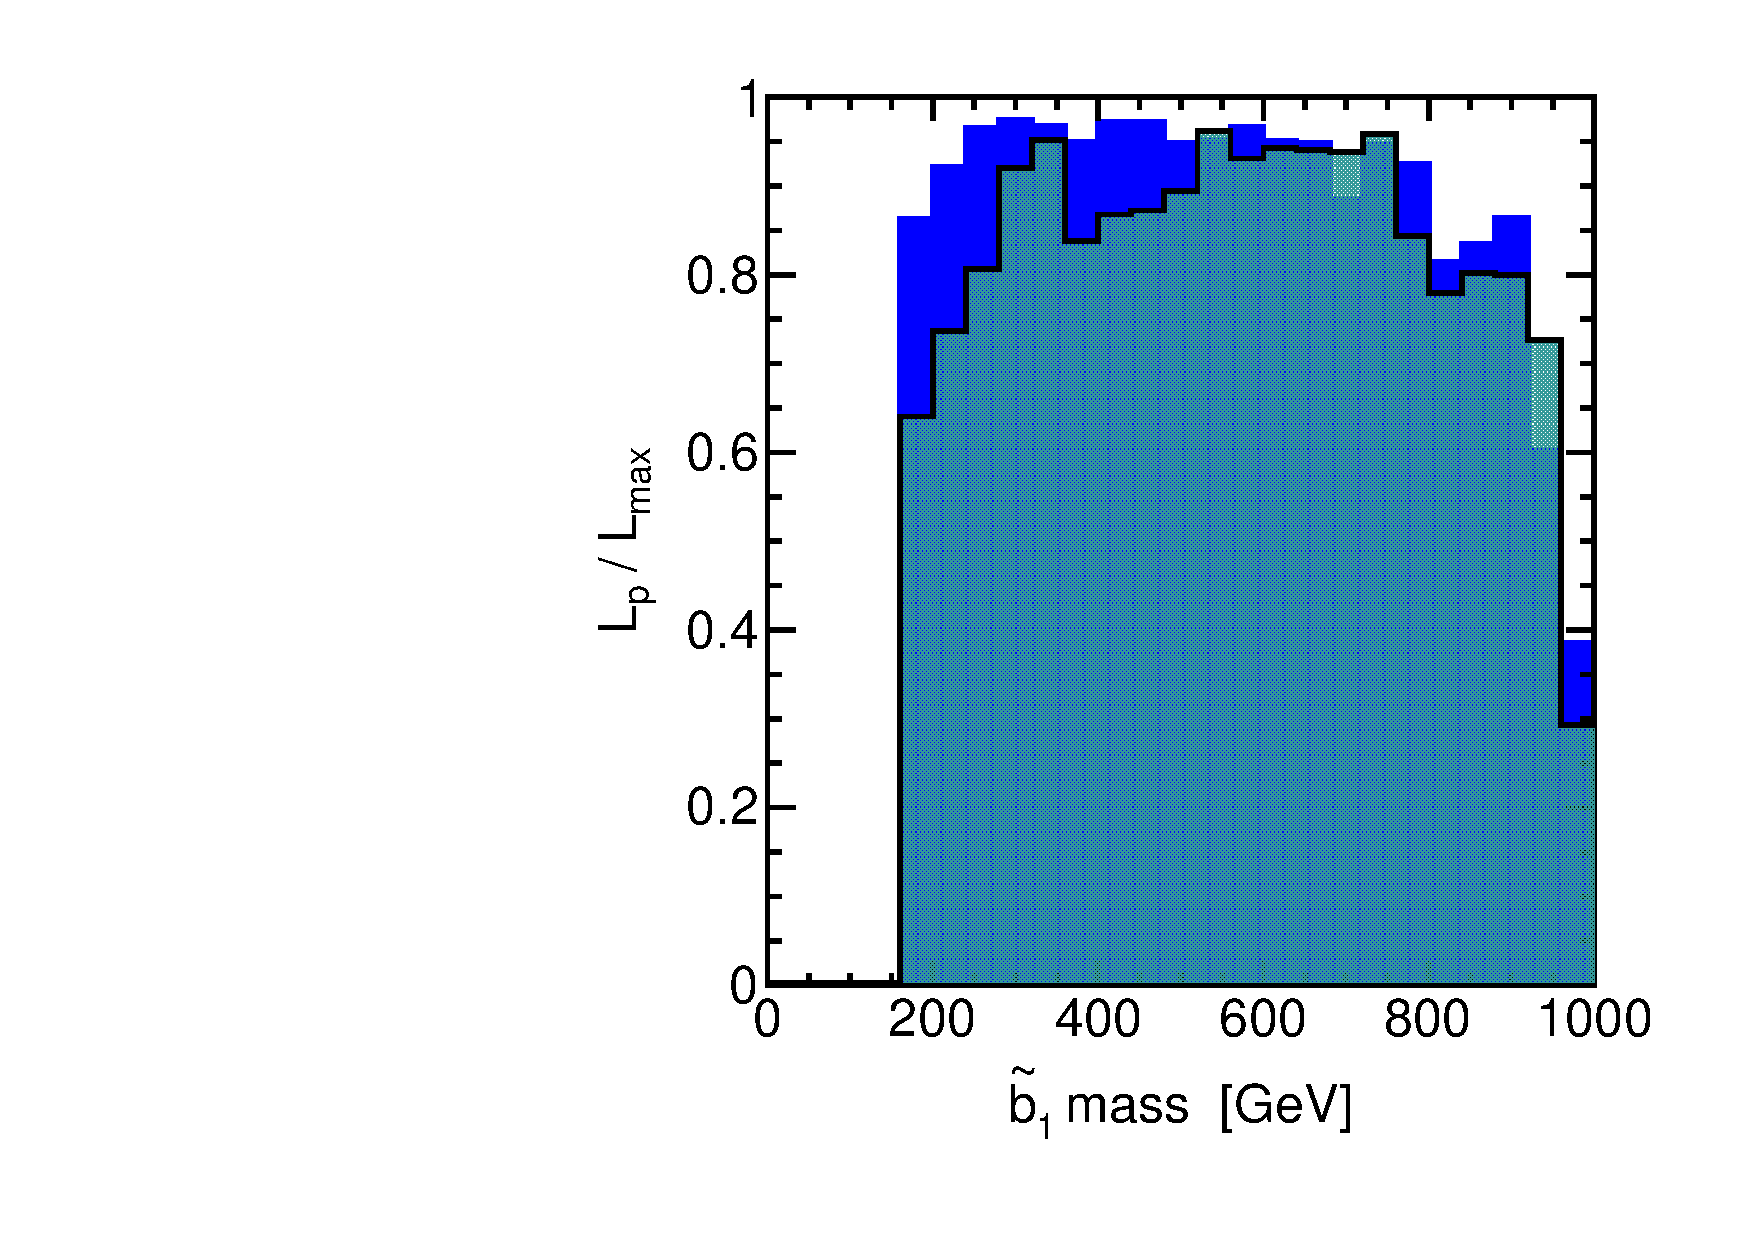
\includegraphics[height=5.5cm]{figs/fig_b_1.pdf} 
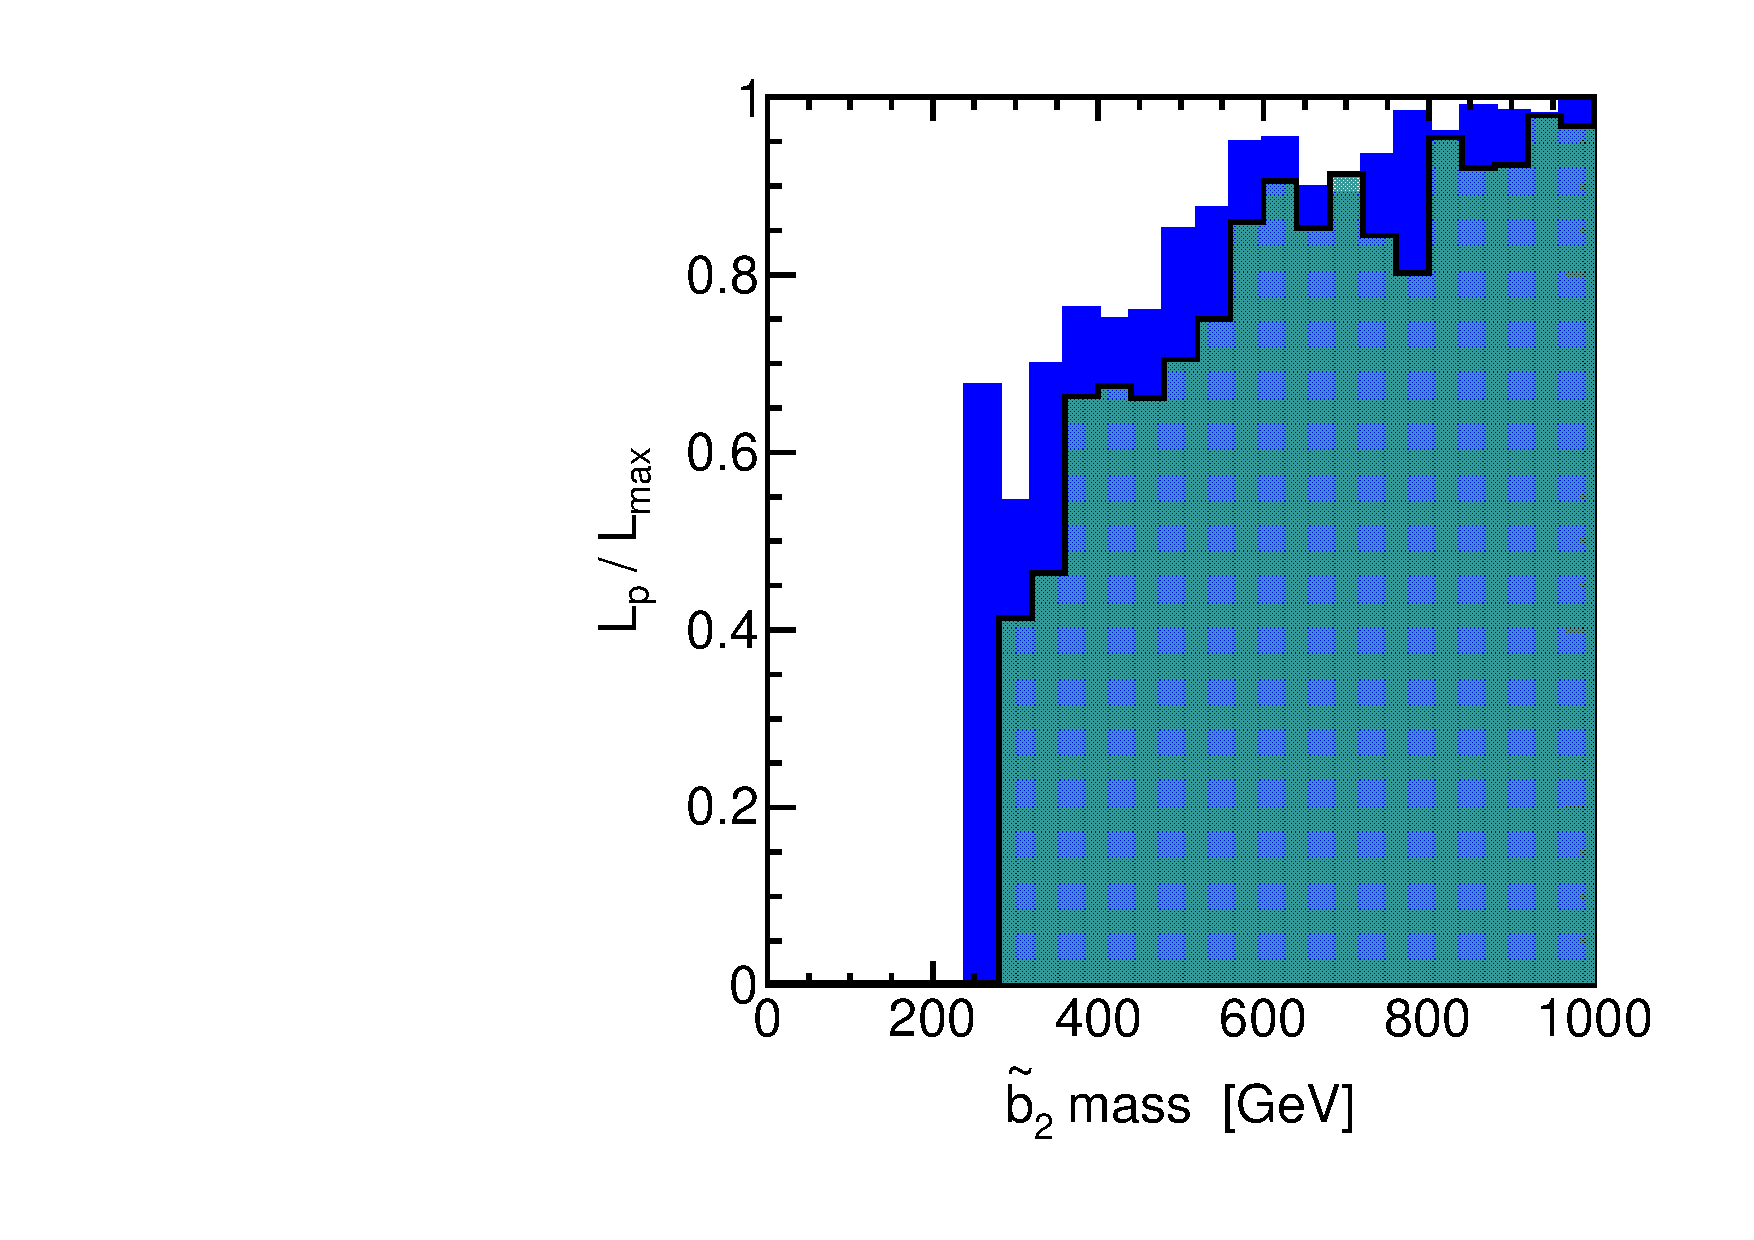
\includegraphics[height=5.5cm]{figs/fig_b_2.pdf} \\
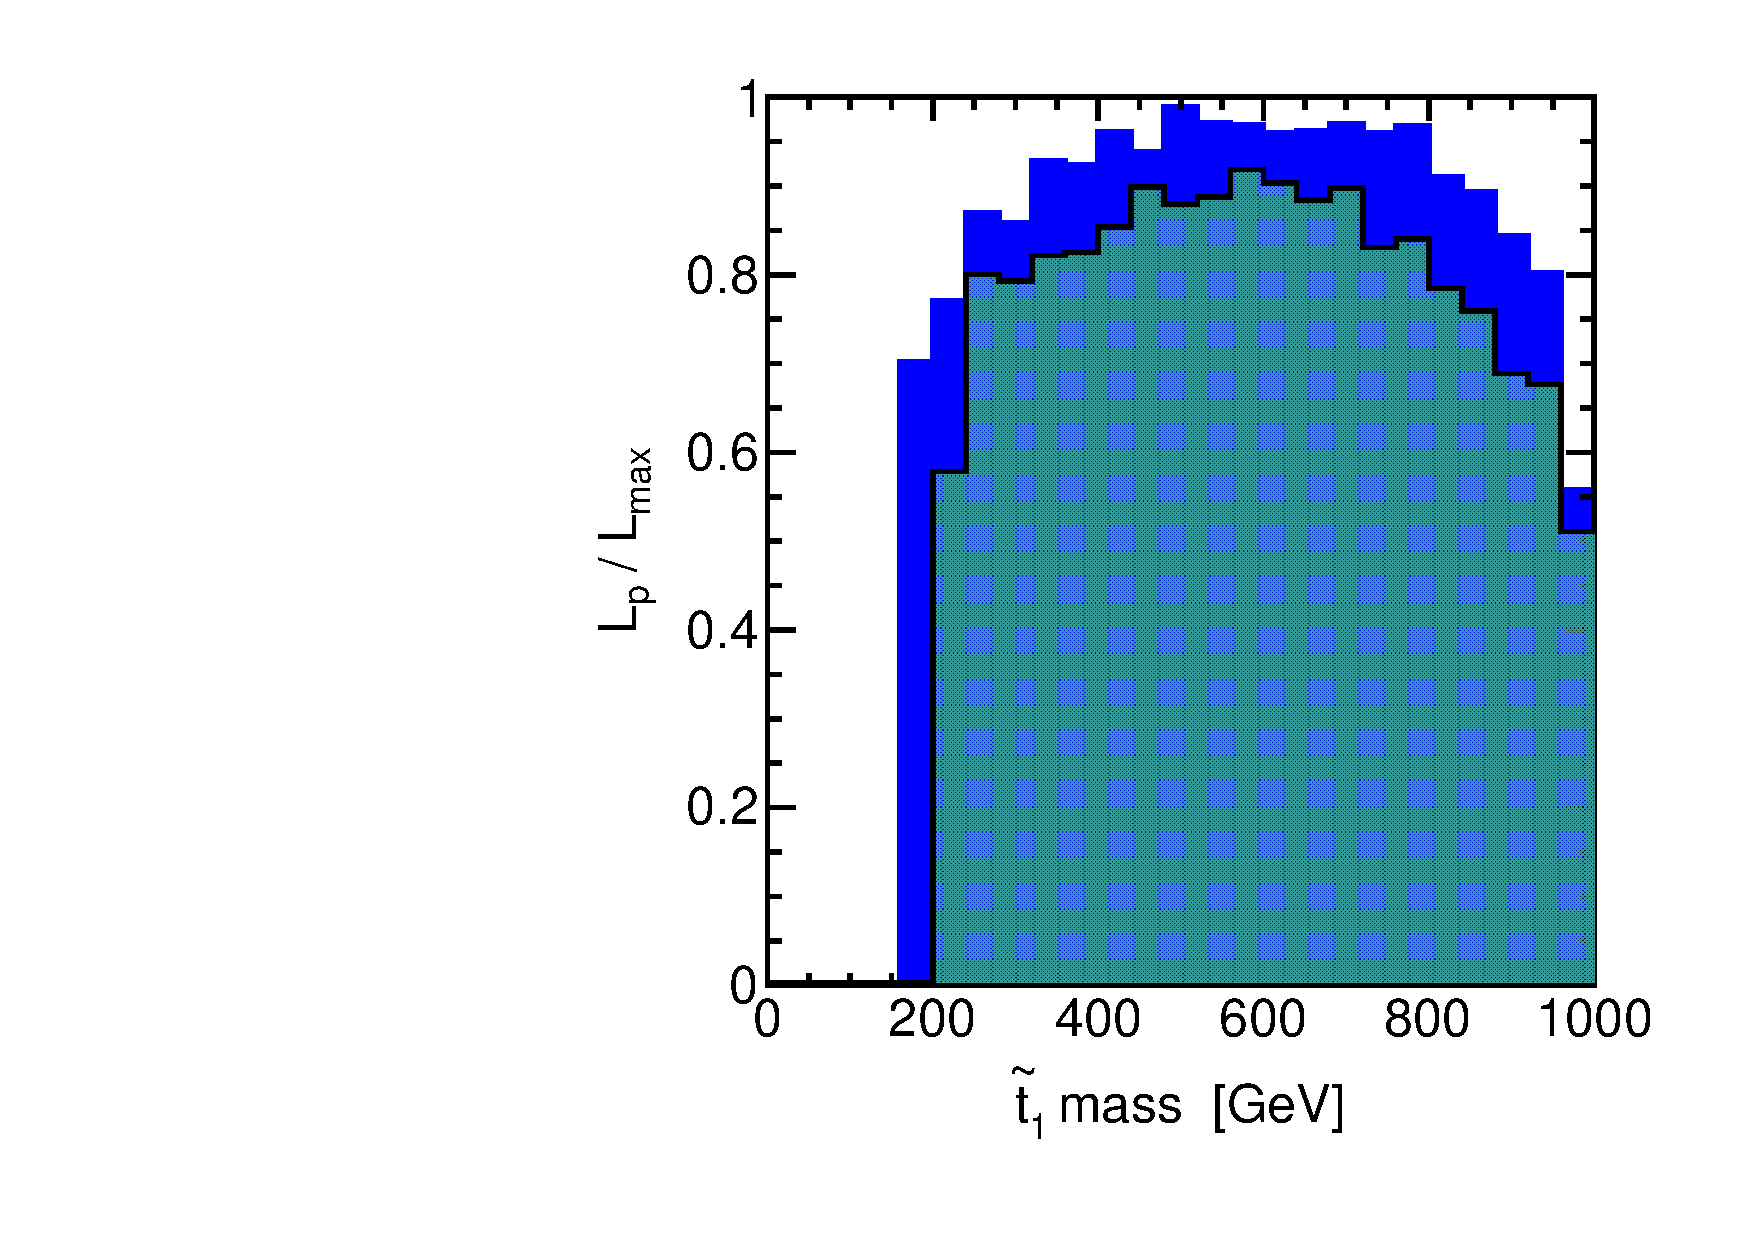
\includegraphics[height=5.5cm]{figs/fig_t_1.pdf} 
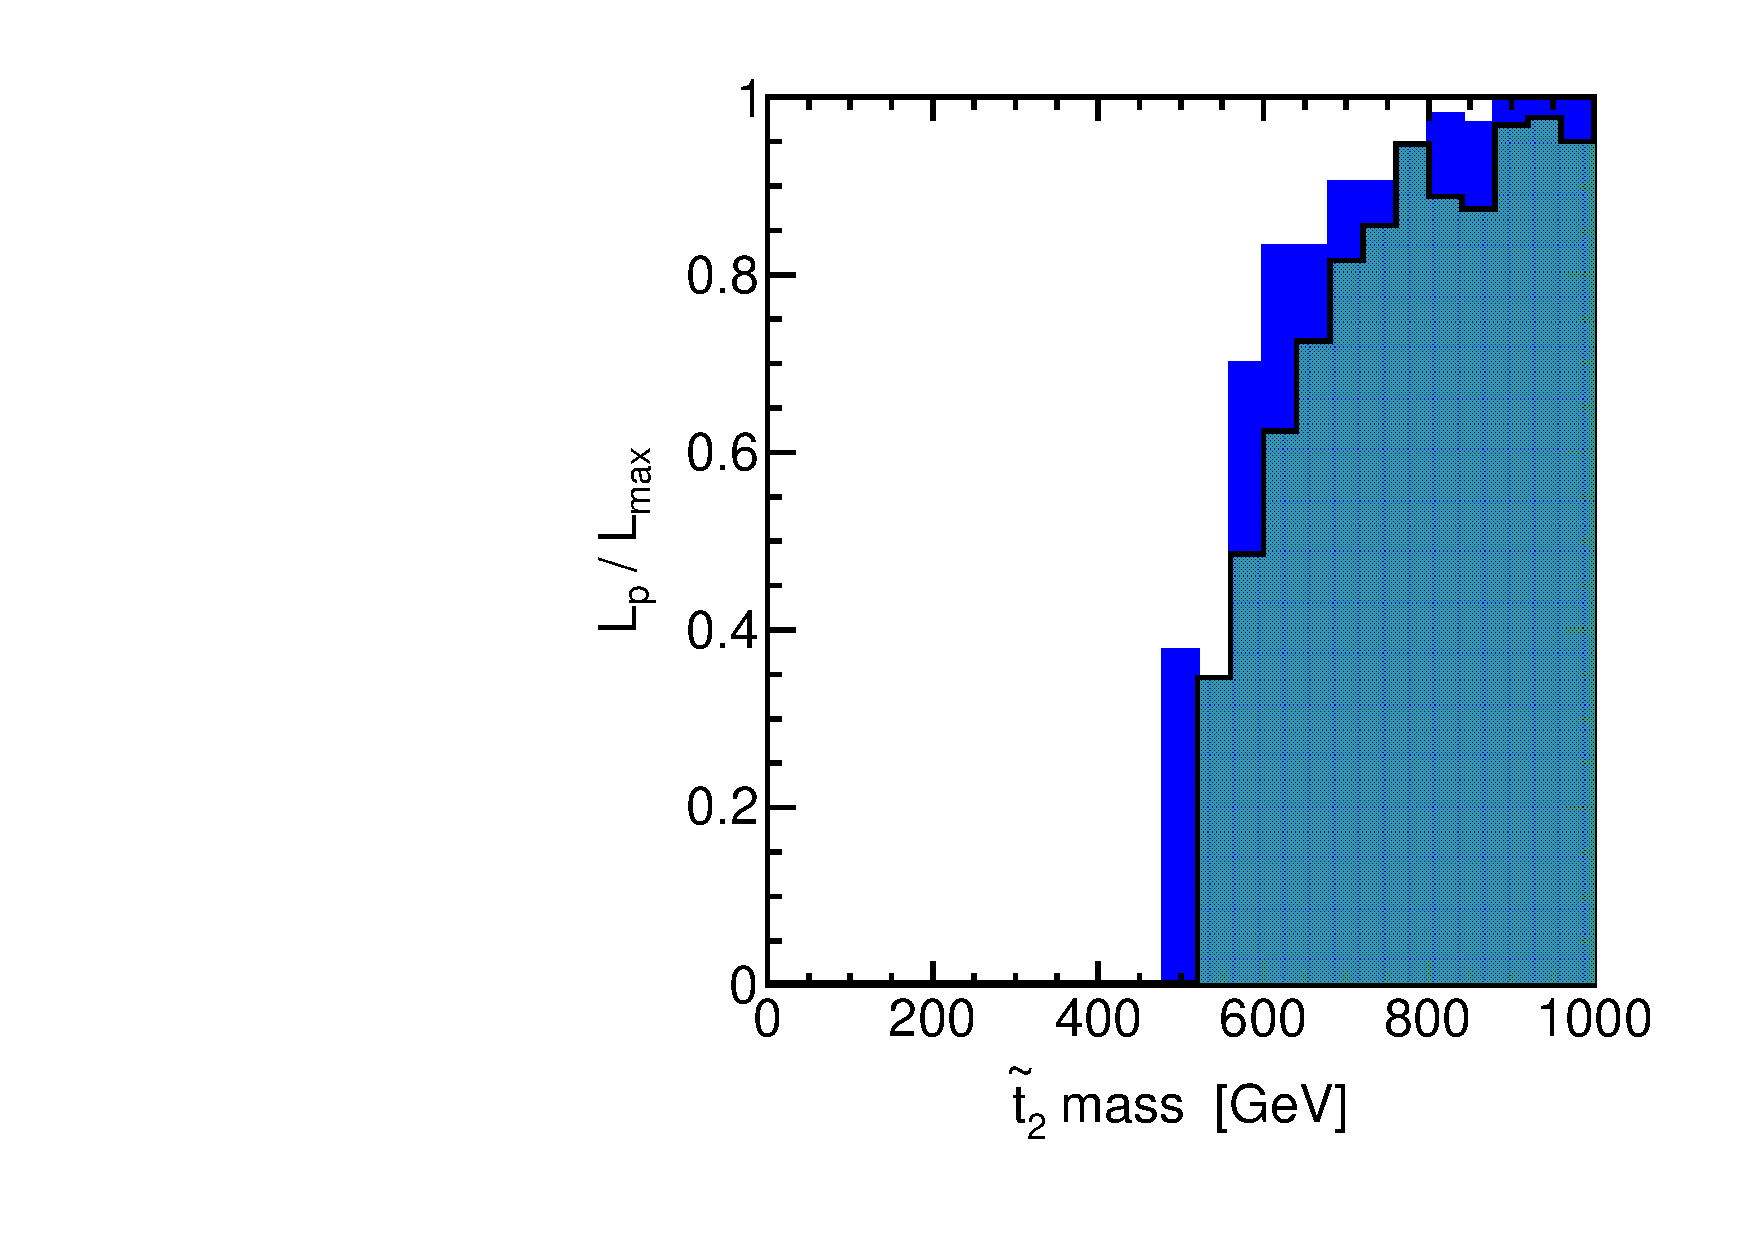
\includegraphics[height=5.5cm]{figs/fig_t_2.pdf} \\
\caption{Ratios of profile likelihood $L_p$ to maximum likelihood $L_{max}$ shown for squark masses.  The colored and shaded histograms show the distributions before and after the inclusion of the CMS results.}
\label{fig:LRwcms_sq}
\end{center}
\end{figure}


\begin{figure}[htbp]
\begin{center}
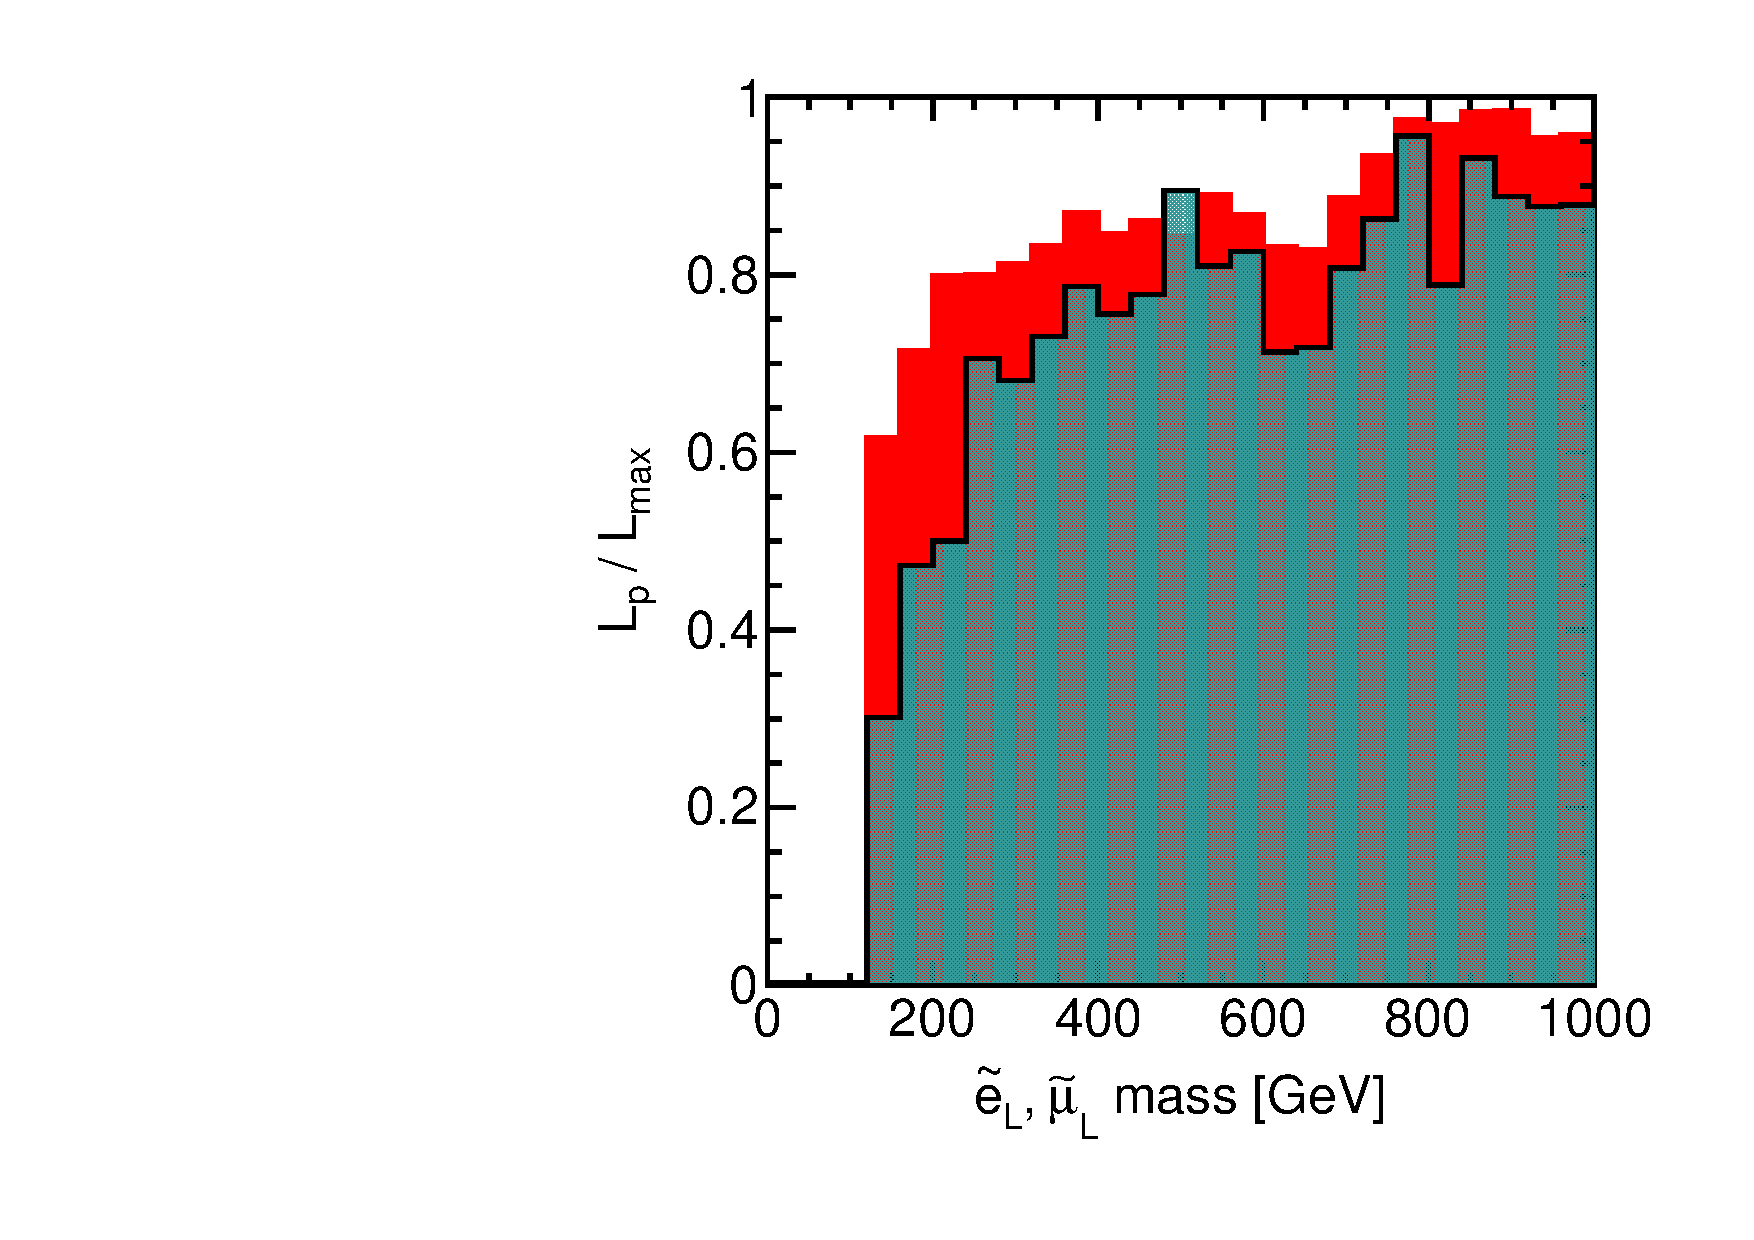
\includegraphics[height=5.5cm]{figs/fig_e_L.pdf} 
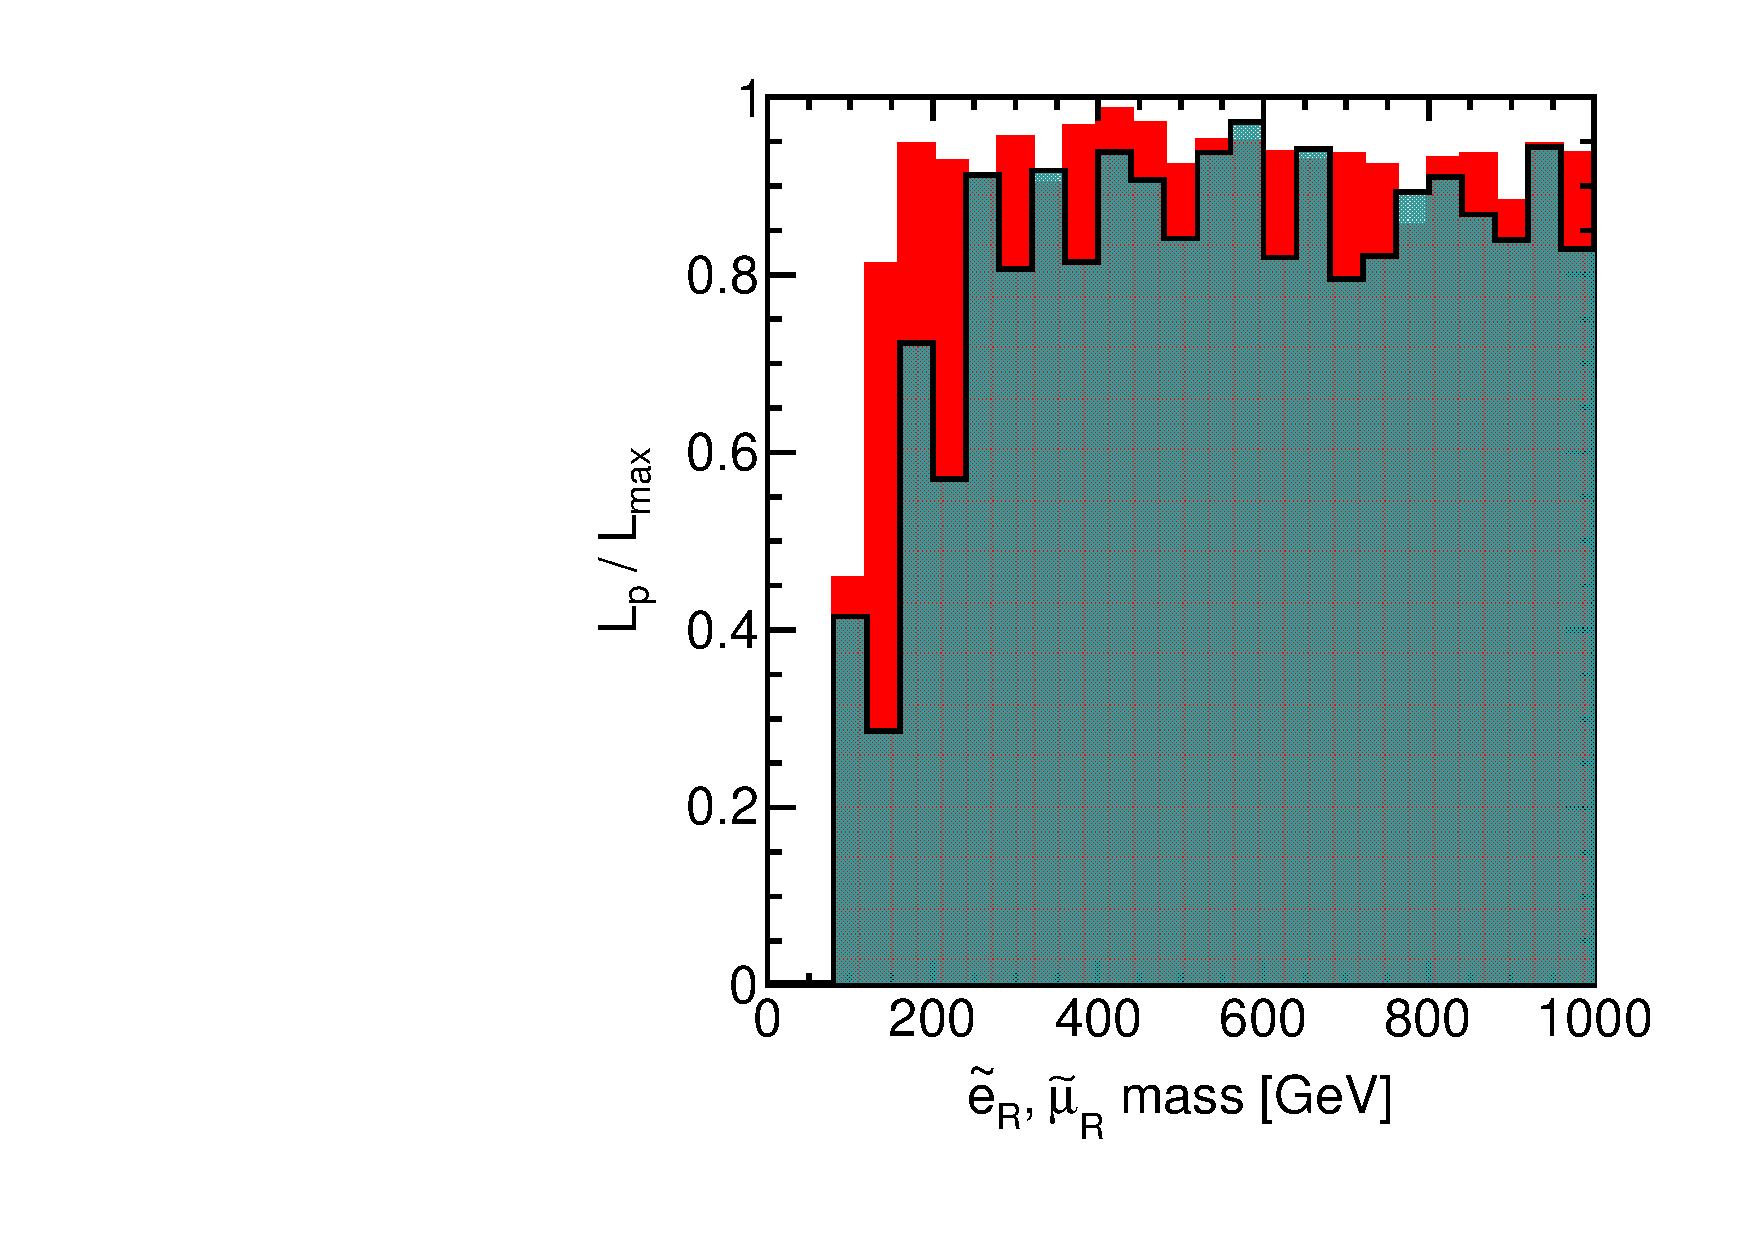
\includegraphics[height=5.5cm]{figs/fig_e_R.pdf} \\
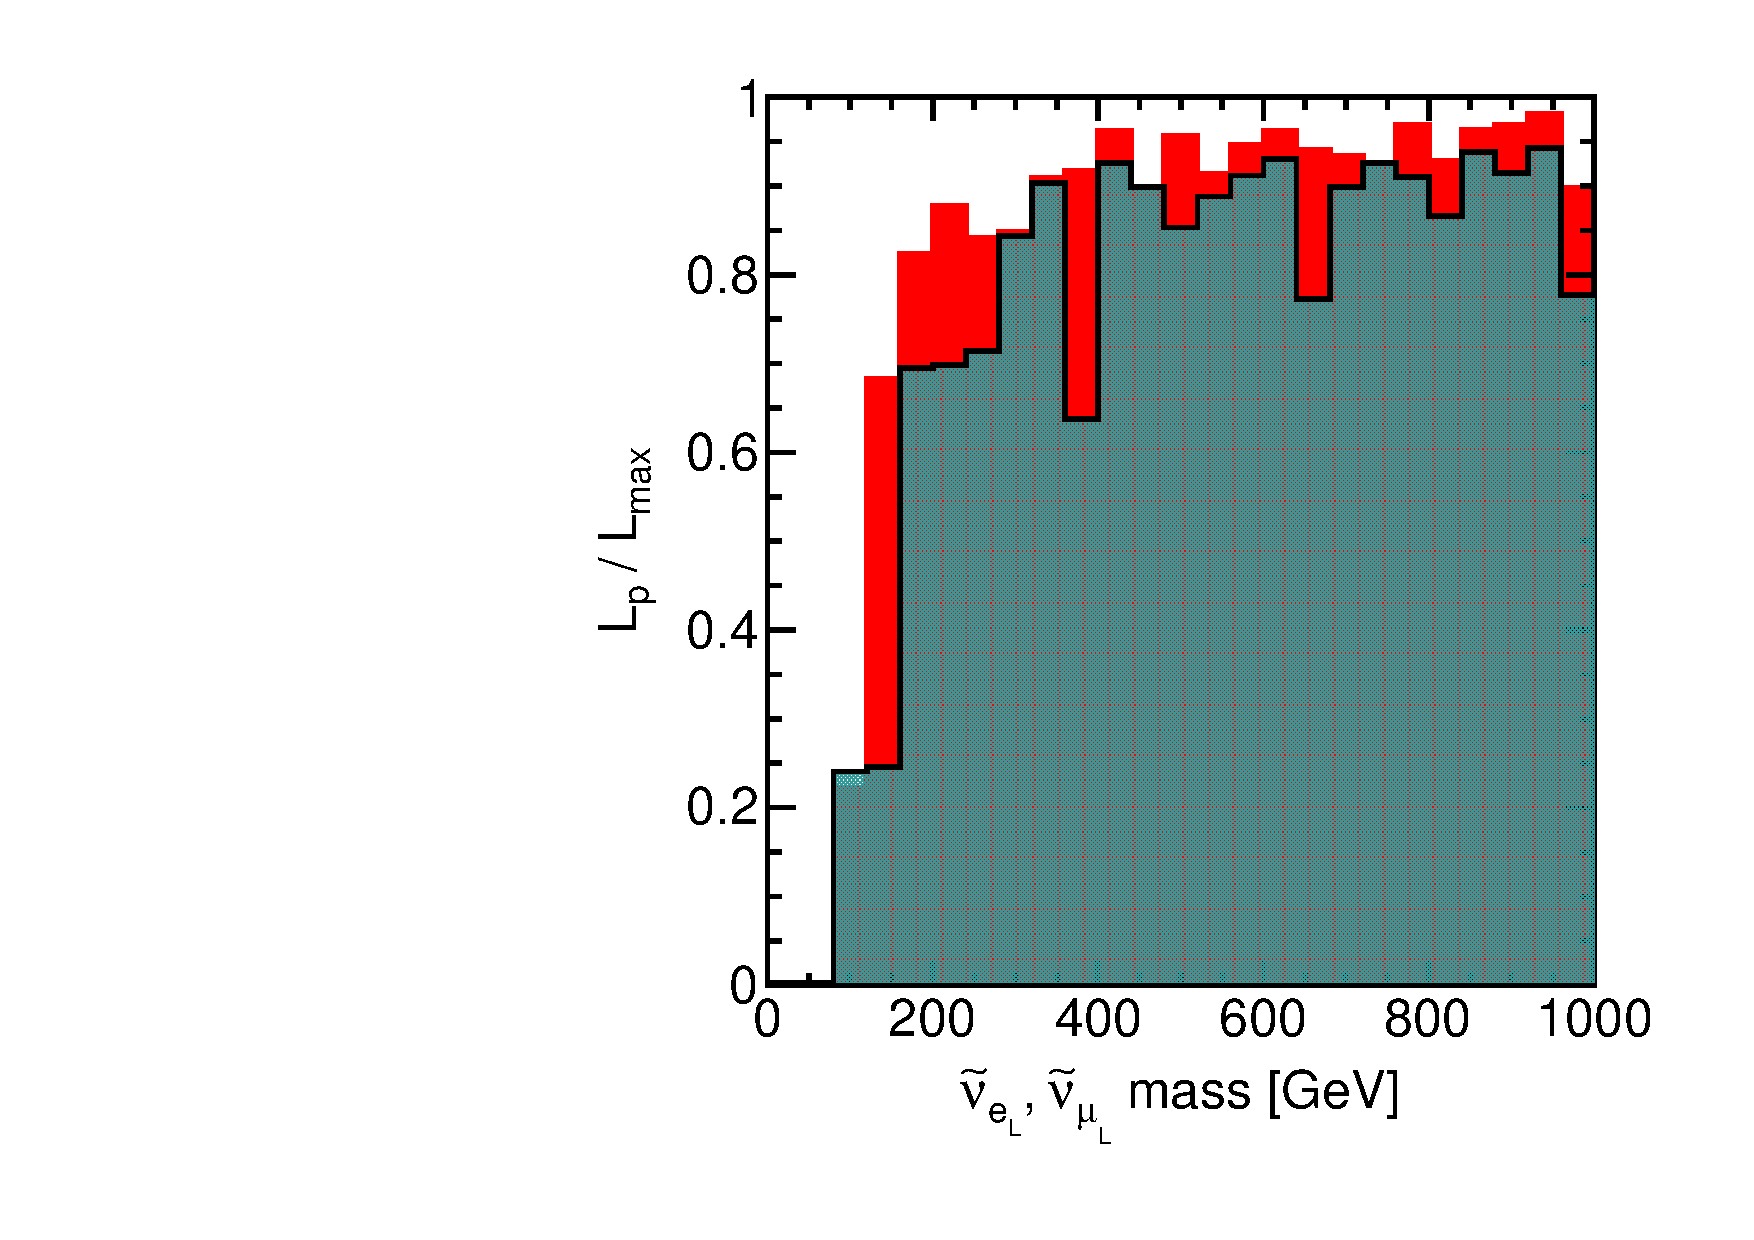
\includegraphics[height=5.5cm]{figs/fig_nu_e_L.pdf} 
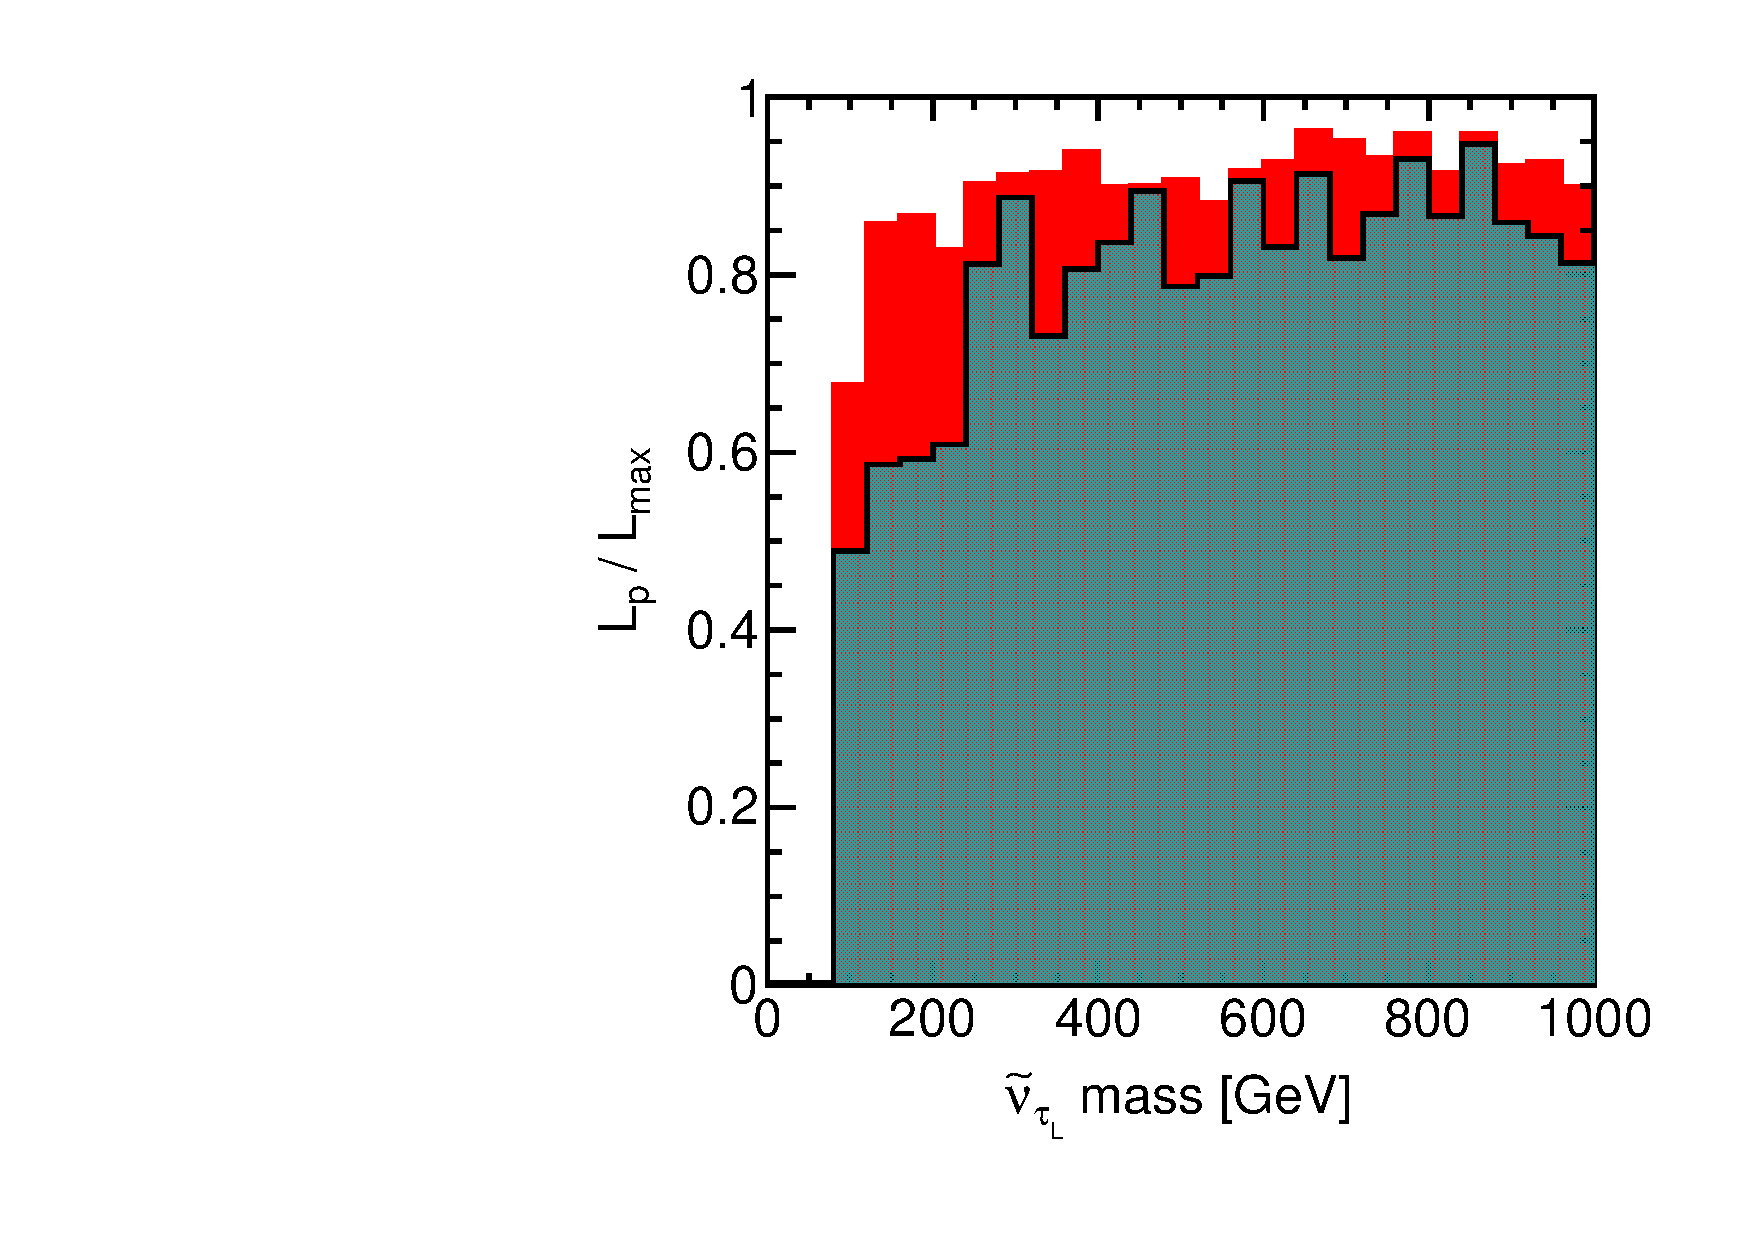
\includegraphics[height=5.5cm]{figs/fig_nu_tau_L.pdf} \\
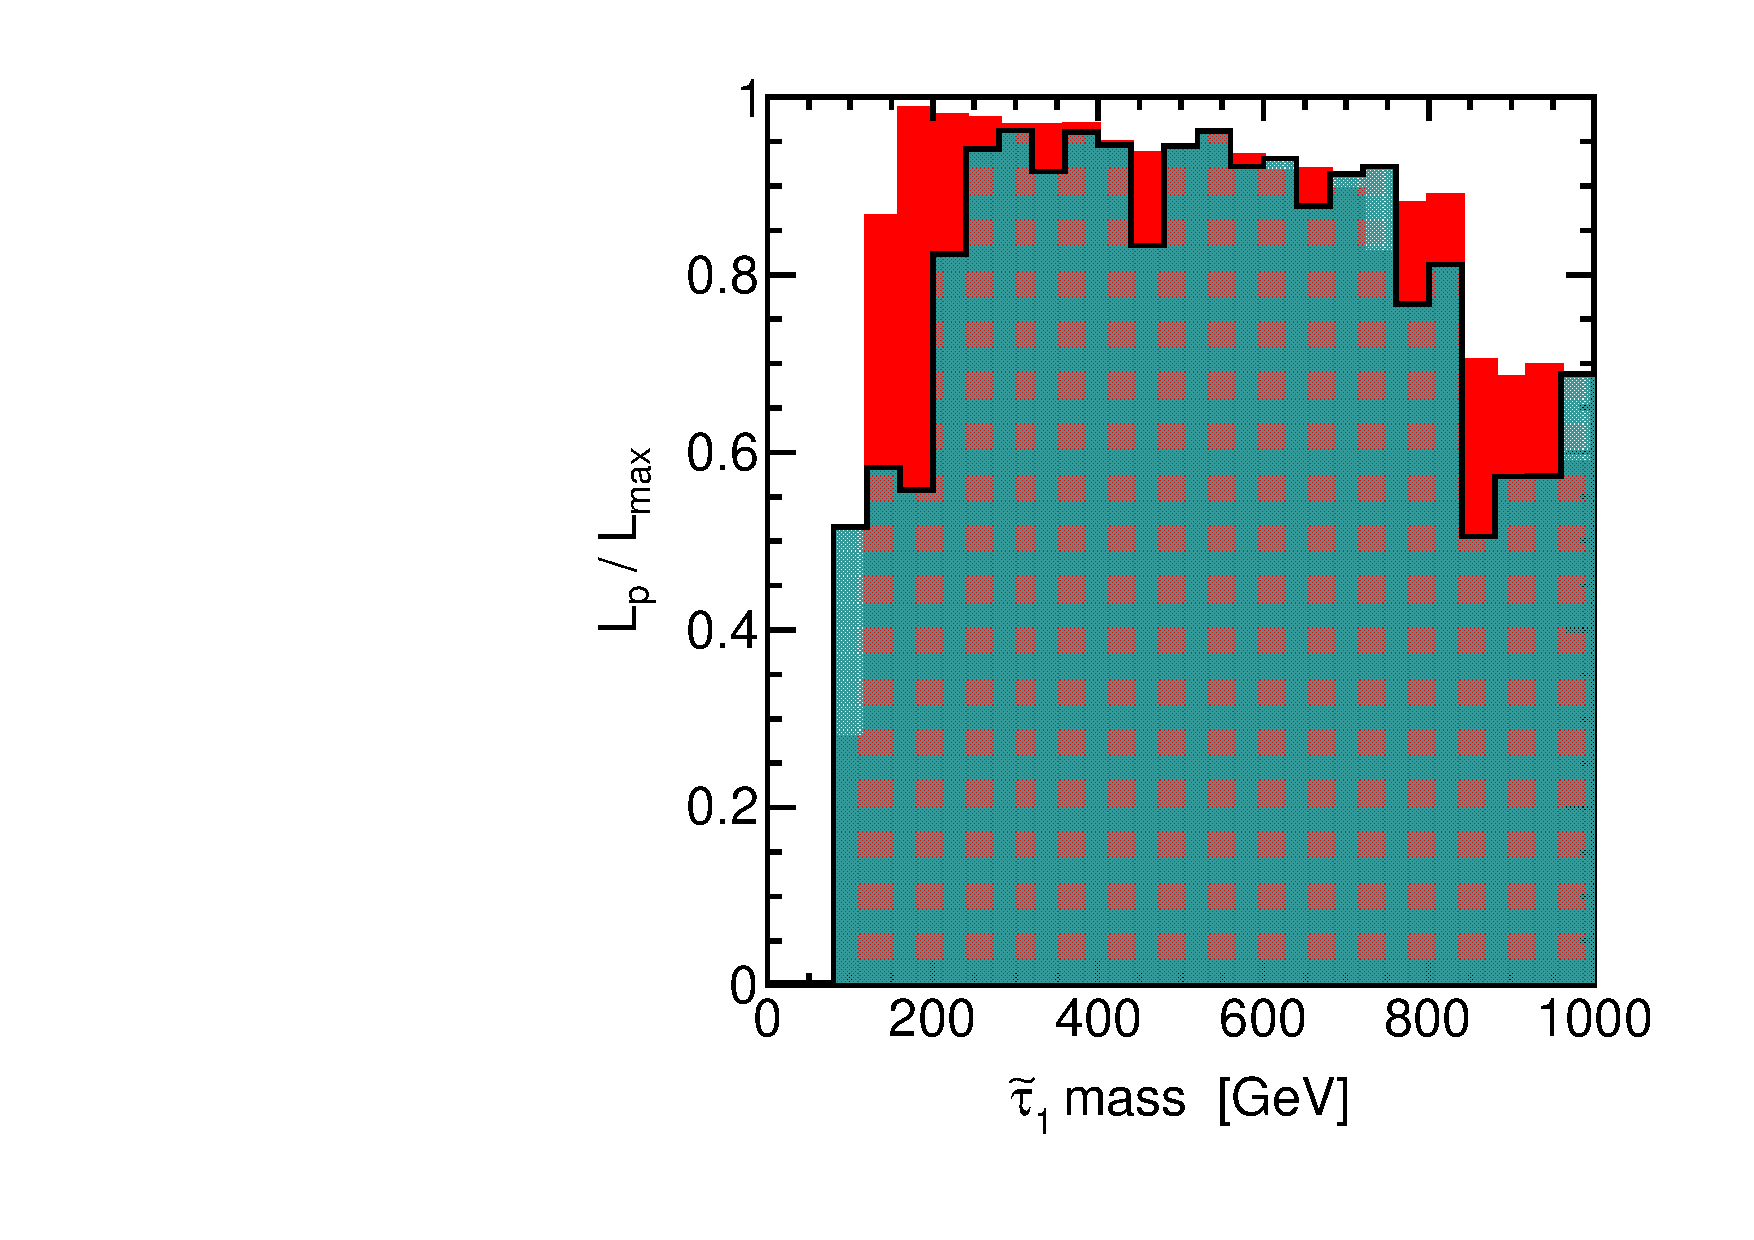
\includegraphics[height=5.5cm]{figs/fig_tau_1.pdf} 
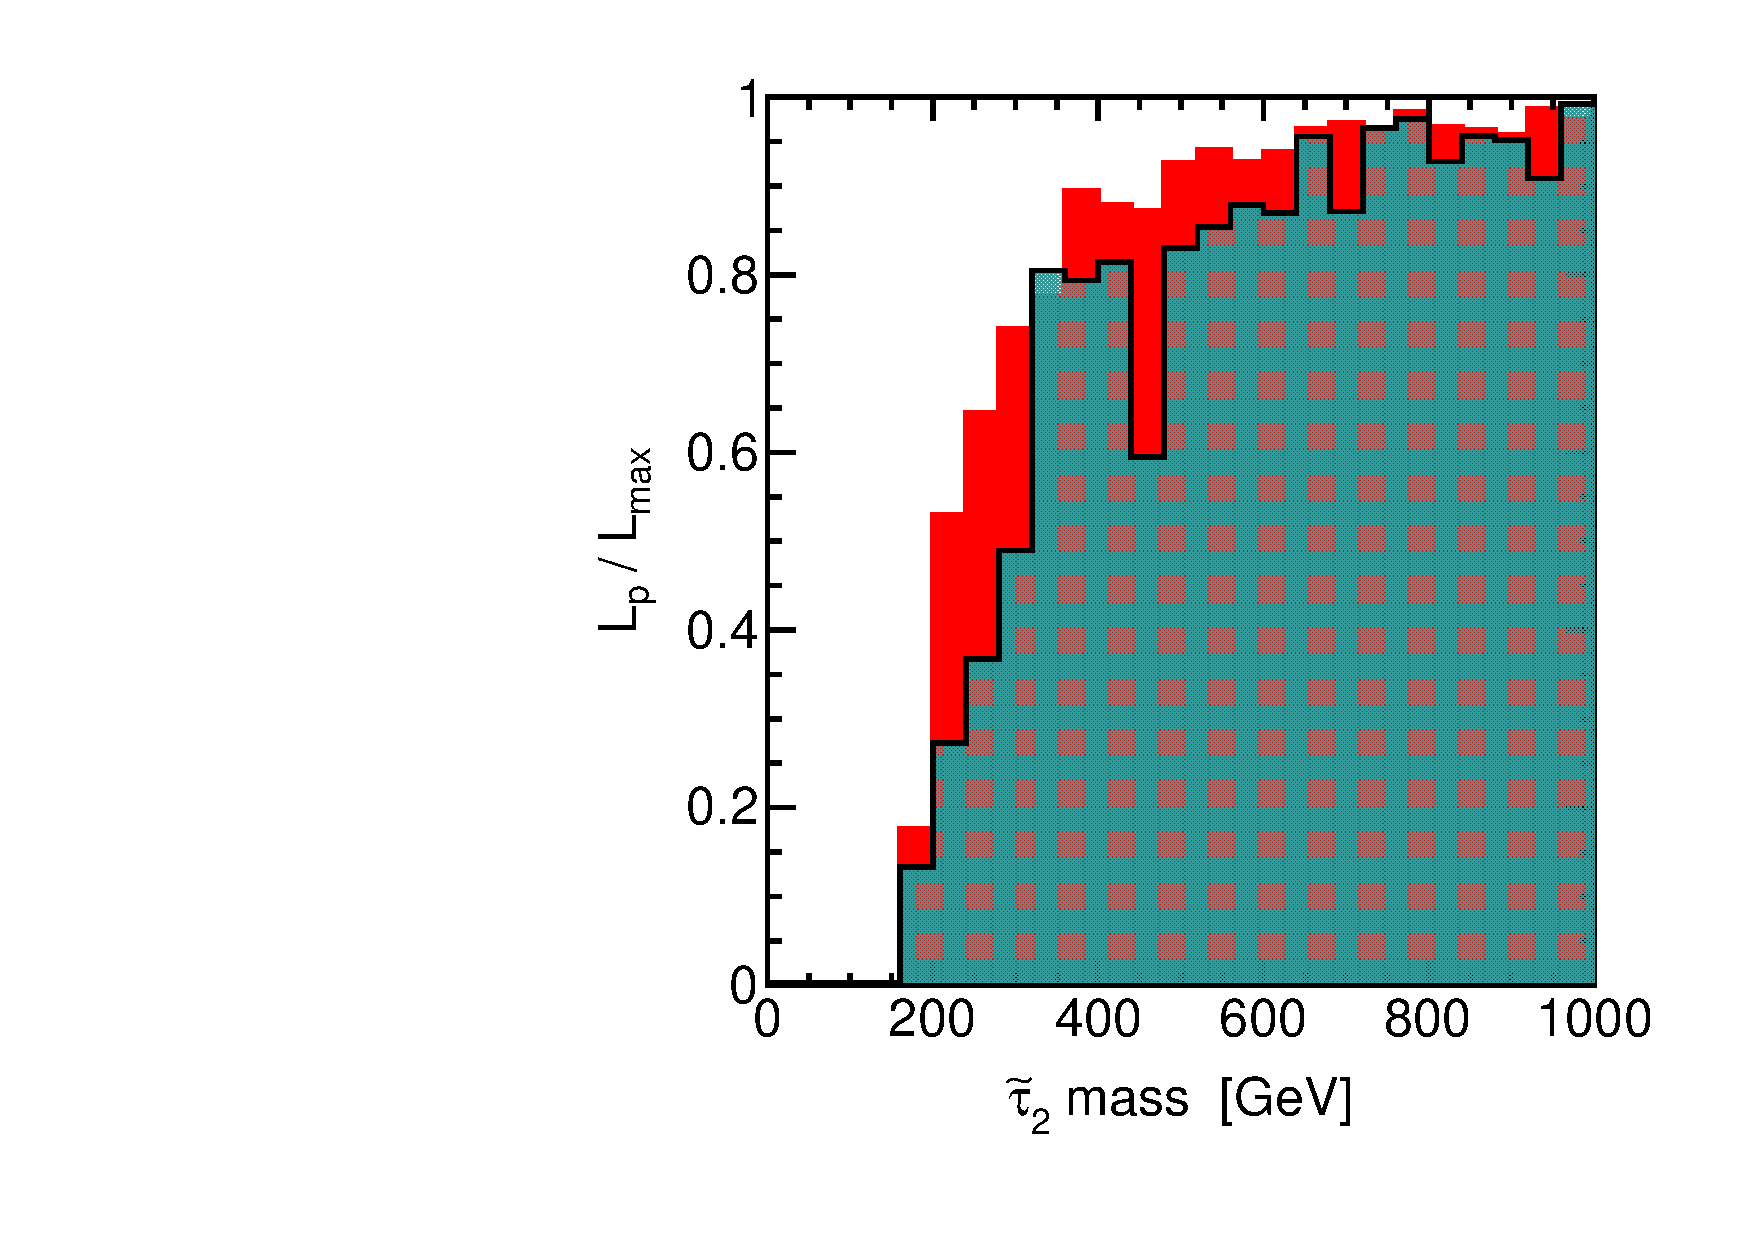
\includegraphics[height=5.5cm]{figs/fig_tau_2.pdf}
\caption{Ratios of profile likelihood $L_p$ to maximum likelihood $L_{max}$ shown for predictions for slepton masses.  The colored and shaded histograms show the distributions before and after the inclusion of the CMS results.}
\label{fig:LRwcms:sl}
\end{center}
\end{figure}

\begin{figure}[htbp]
\begin{center}
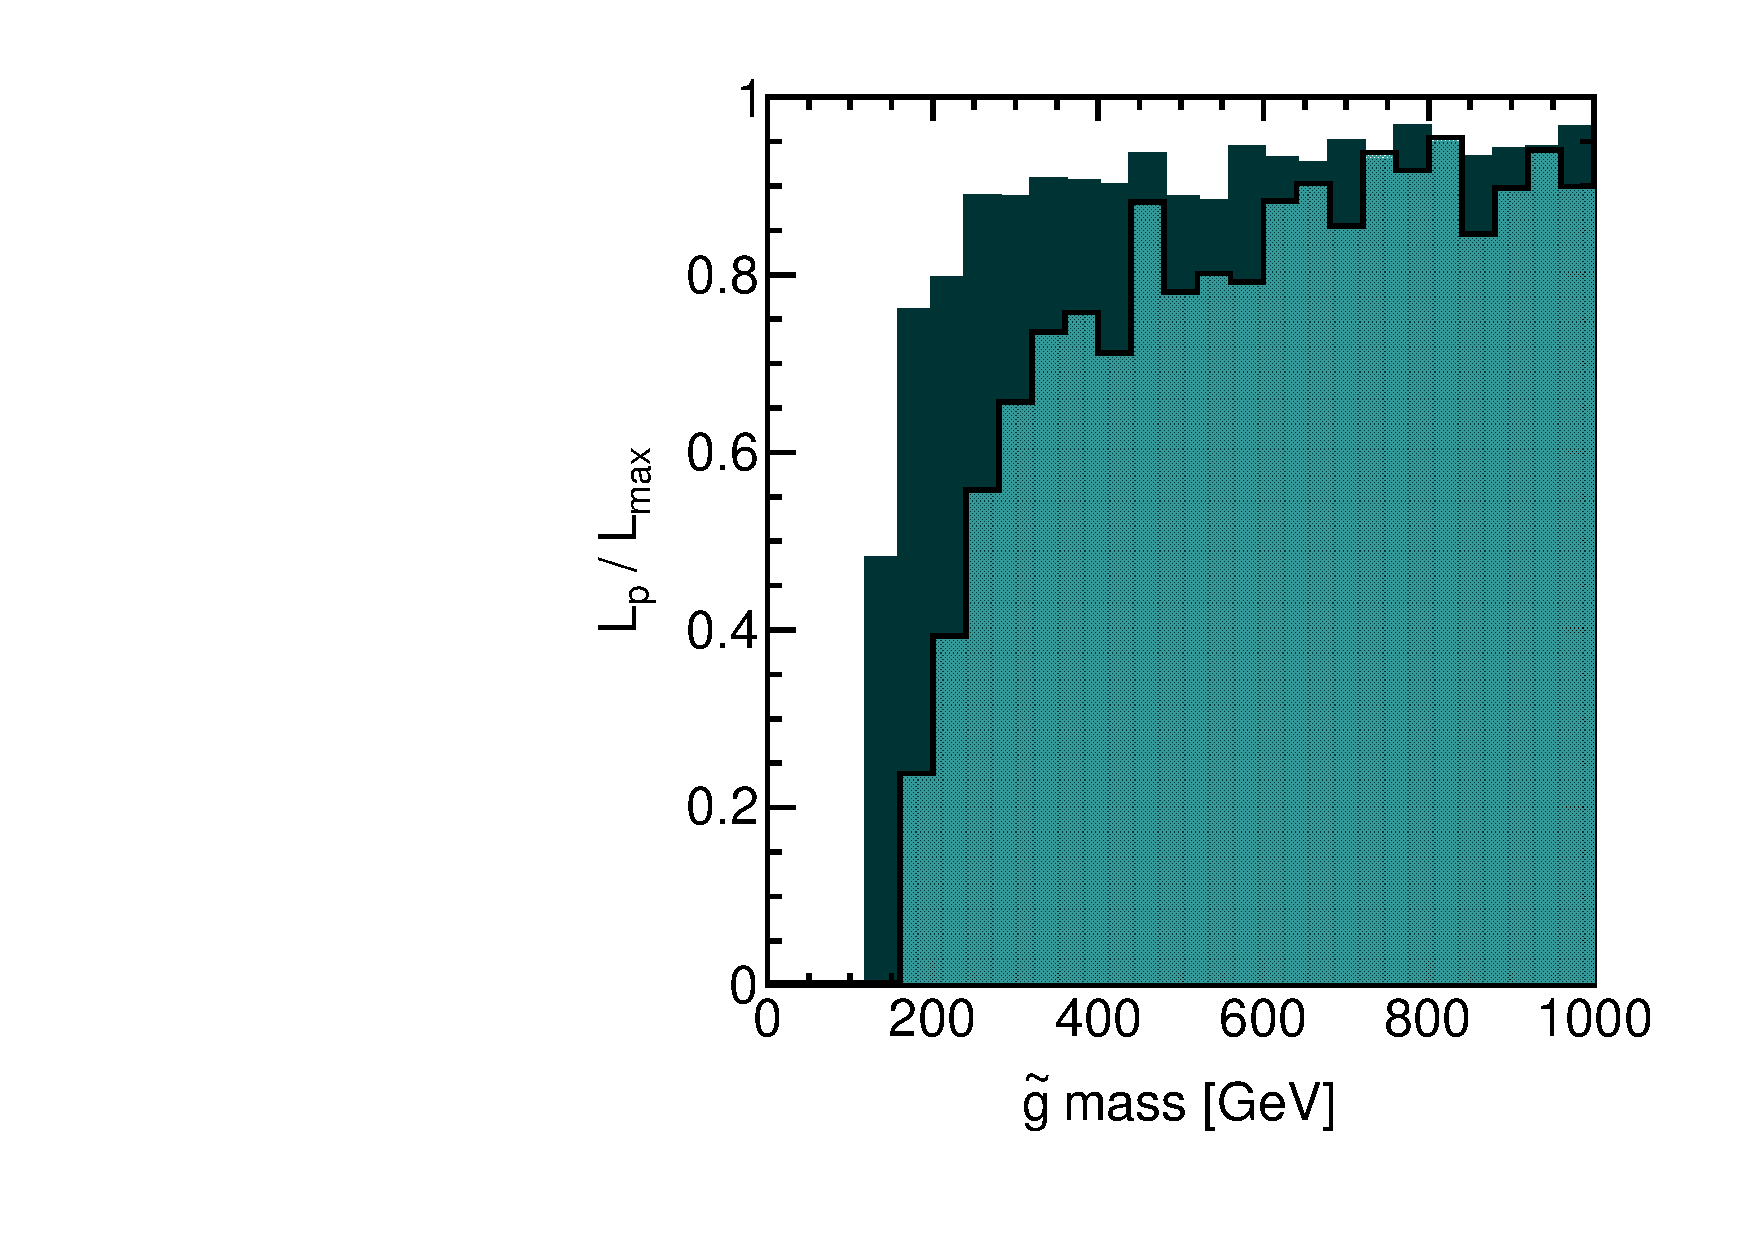
\includegraphics[height=5.5cm]{figs/fig_g.pdf} 
\caption{Ratios of profile likelihood $L_p$ to maximum likelihood $L_{max}$ shown for the gluino mass.  The colored and shaded histograms show the distributions before and after the inclusion of the CMS results.}
\label{fig:LRwcms:g}
\end{center}
\end{figure}


\begin{figure}[htbp]
\begin{center}
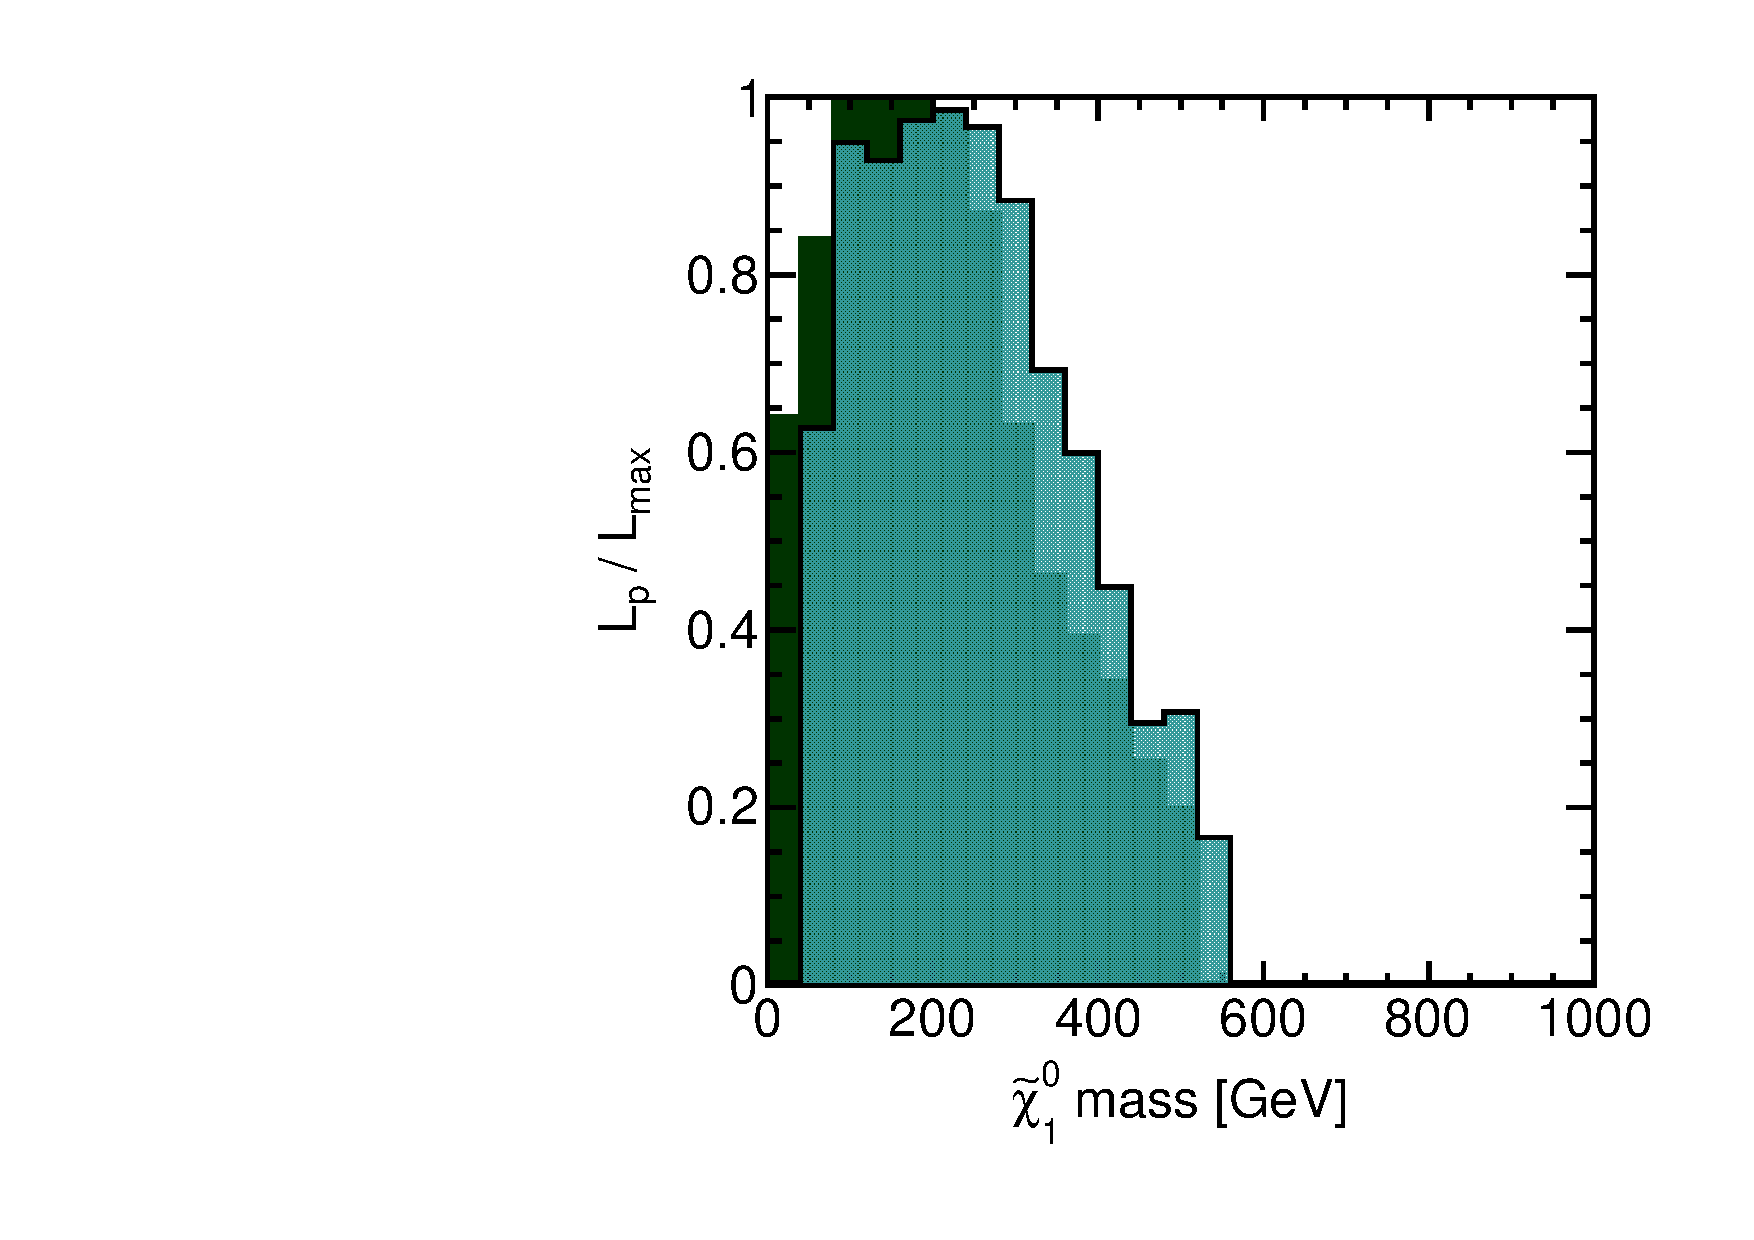
\includegraphics[height=5.5cm]{figs/fig_chi_1_0.pdf} 
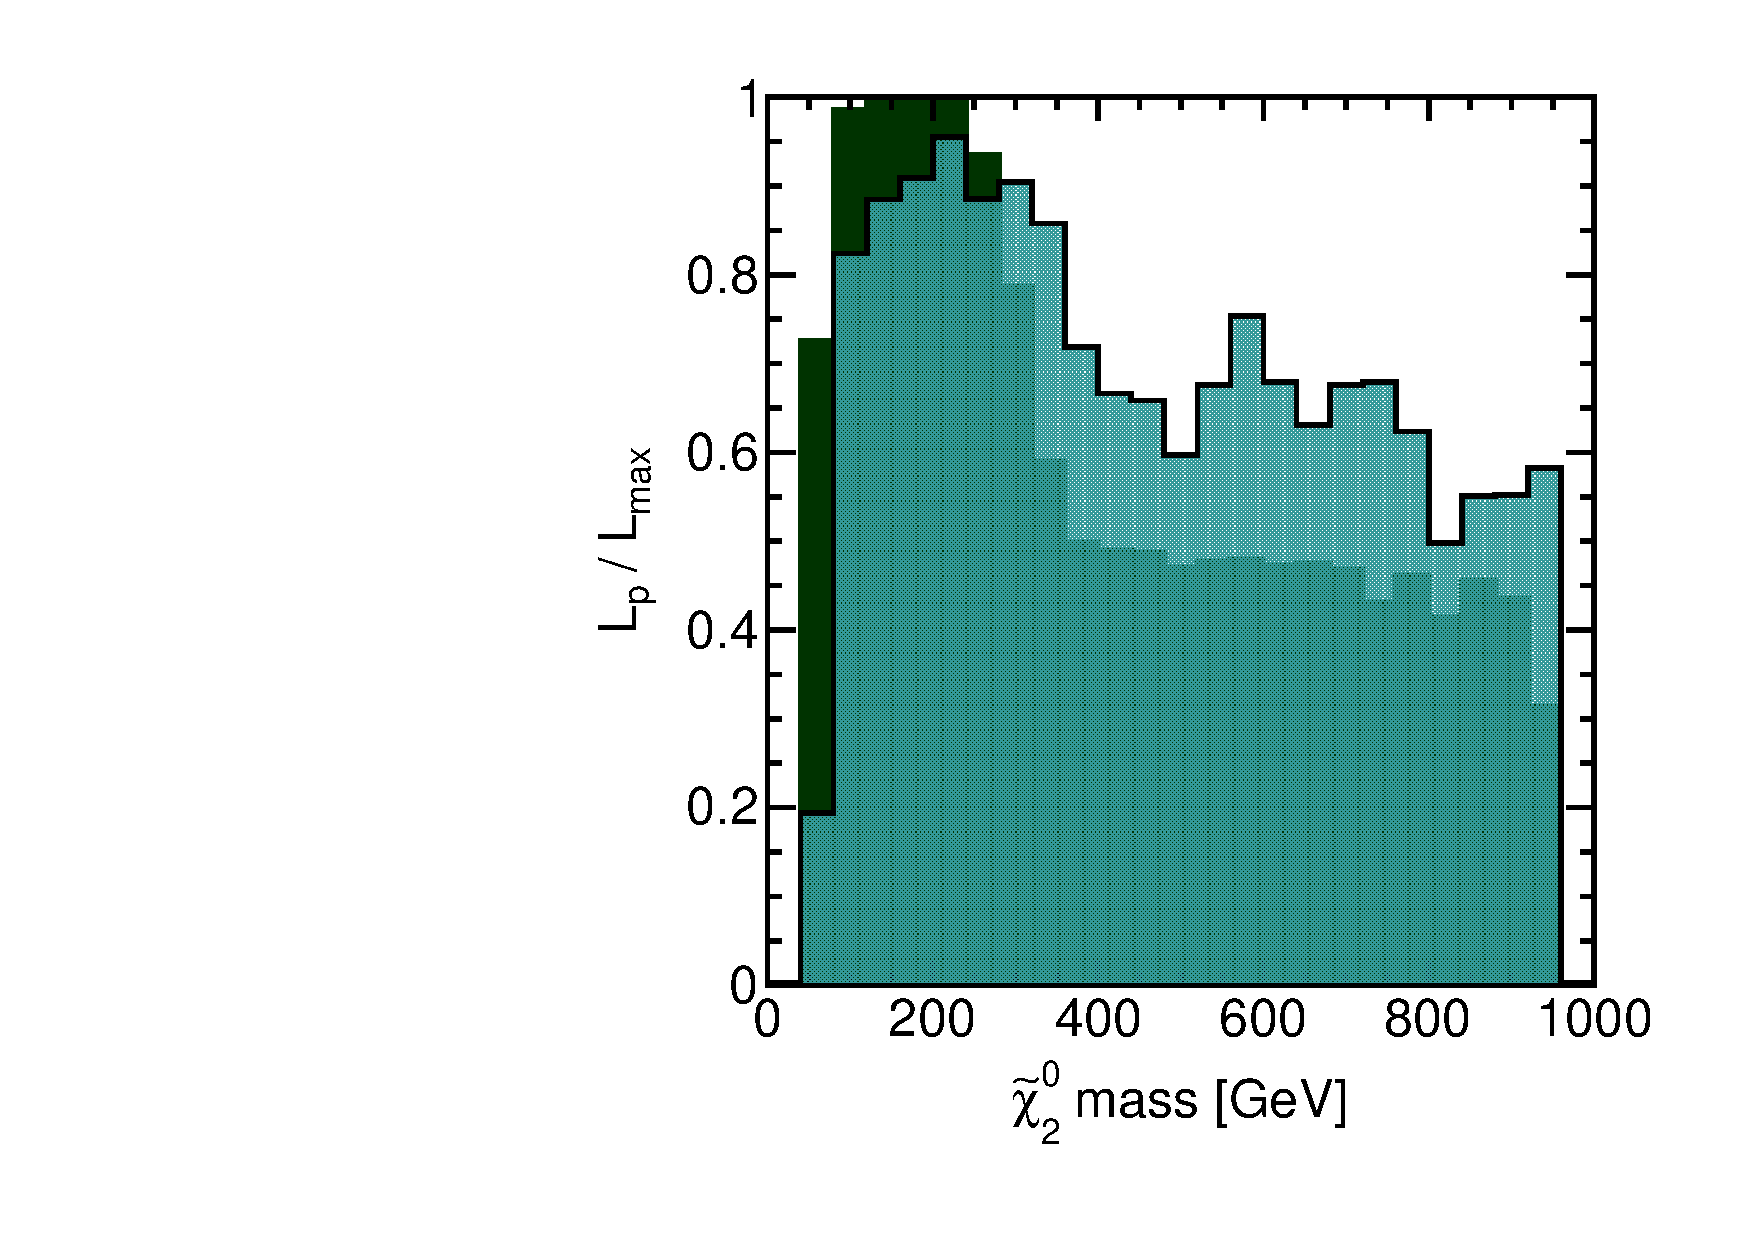
\includegraphics[height=5.5cm]{figs/fig_chi_2_0.pdf} \\
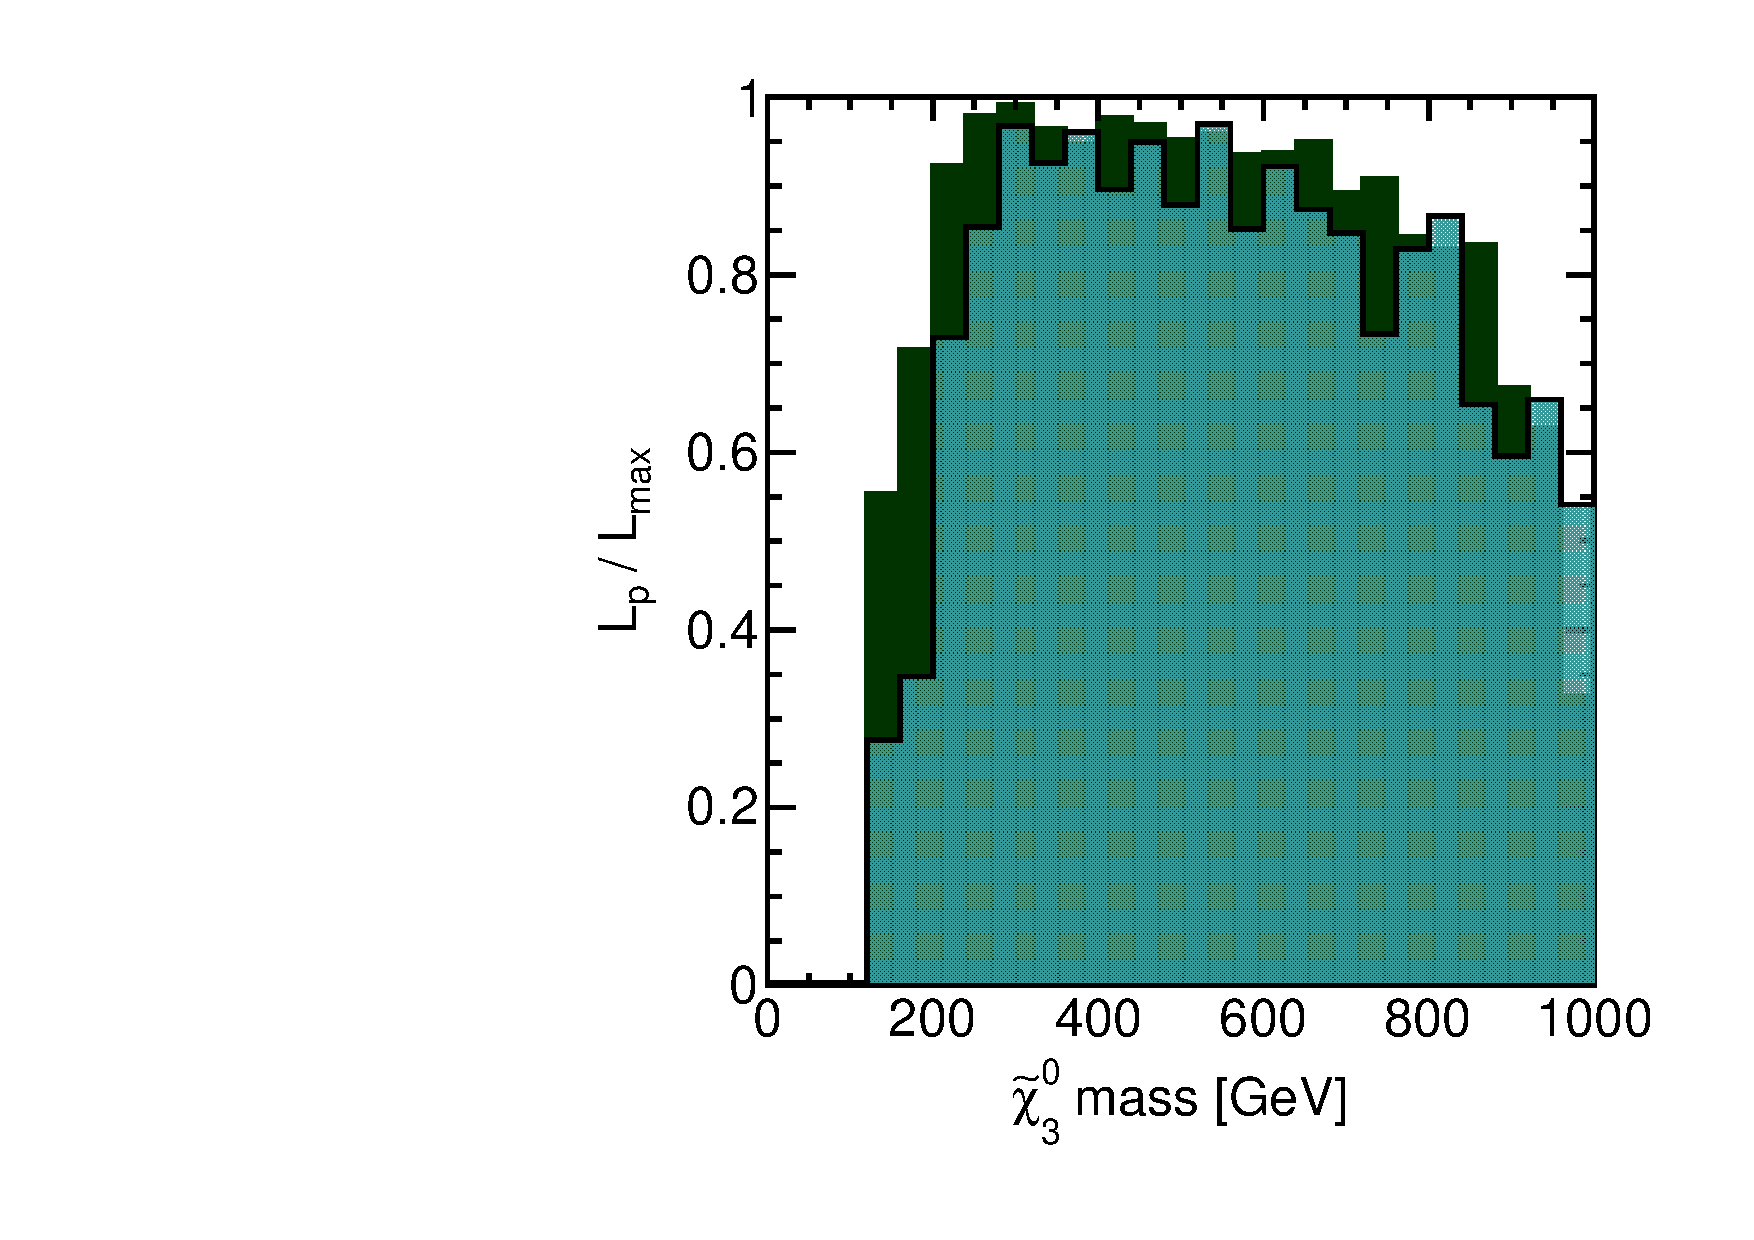
\includegraphics[height=5.5cm]{figs/fig_chi_3_0.pdf} 
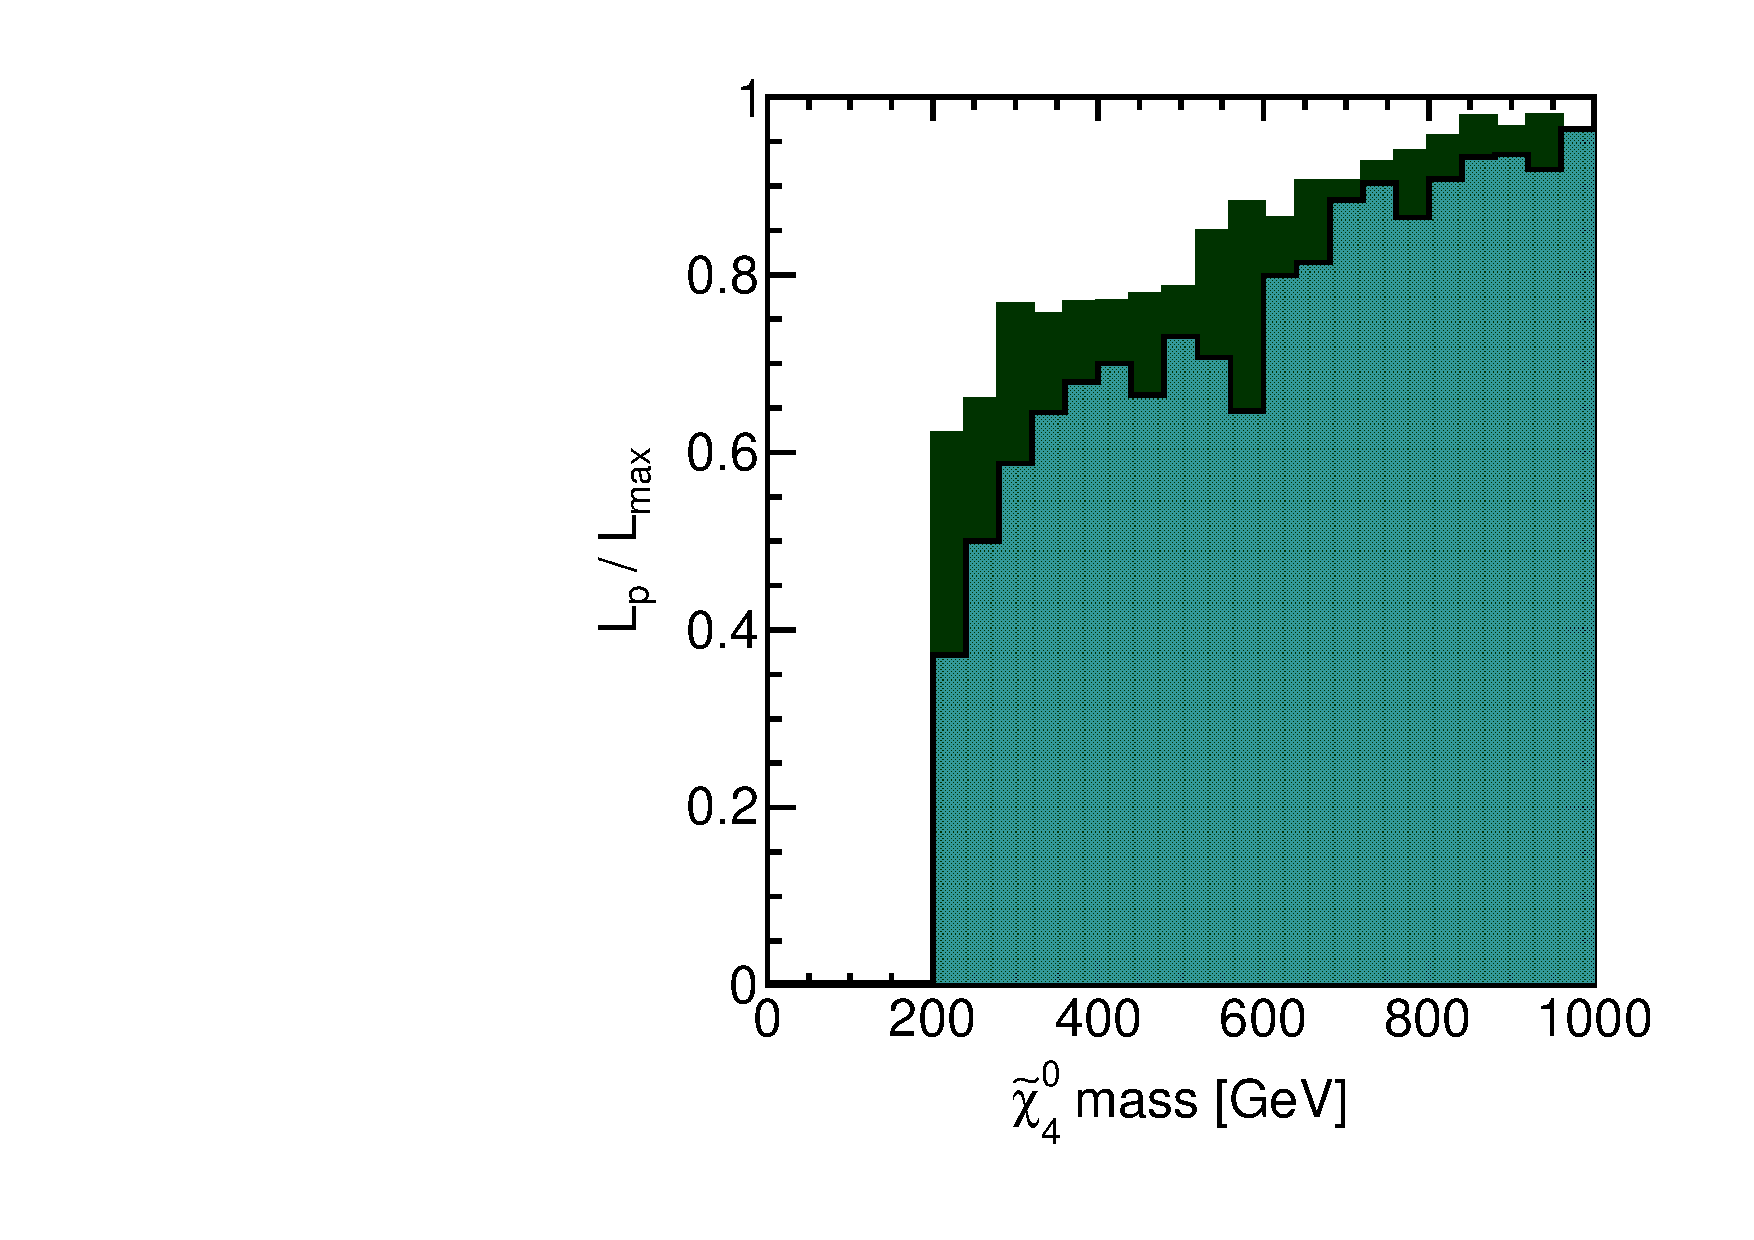
\includegraphics[height=5.5cm]{figs/fig_chi_4_0.pdf} 
\caption{Ratios of profile likelihood $L_p$ to maximum likelihood $L_{max}$ shown for the neutralino masses.  The colored and shaded histograms show the distributions before and after the inclusion of the CMS results.}
\label{fig:LRwcms_chi0}
\end{center}
\end{figure}

\begin{figure}[htbp]
\begin{center}
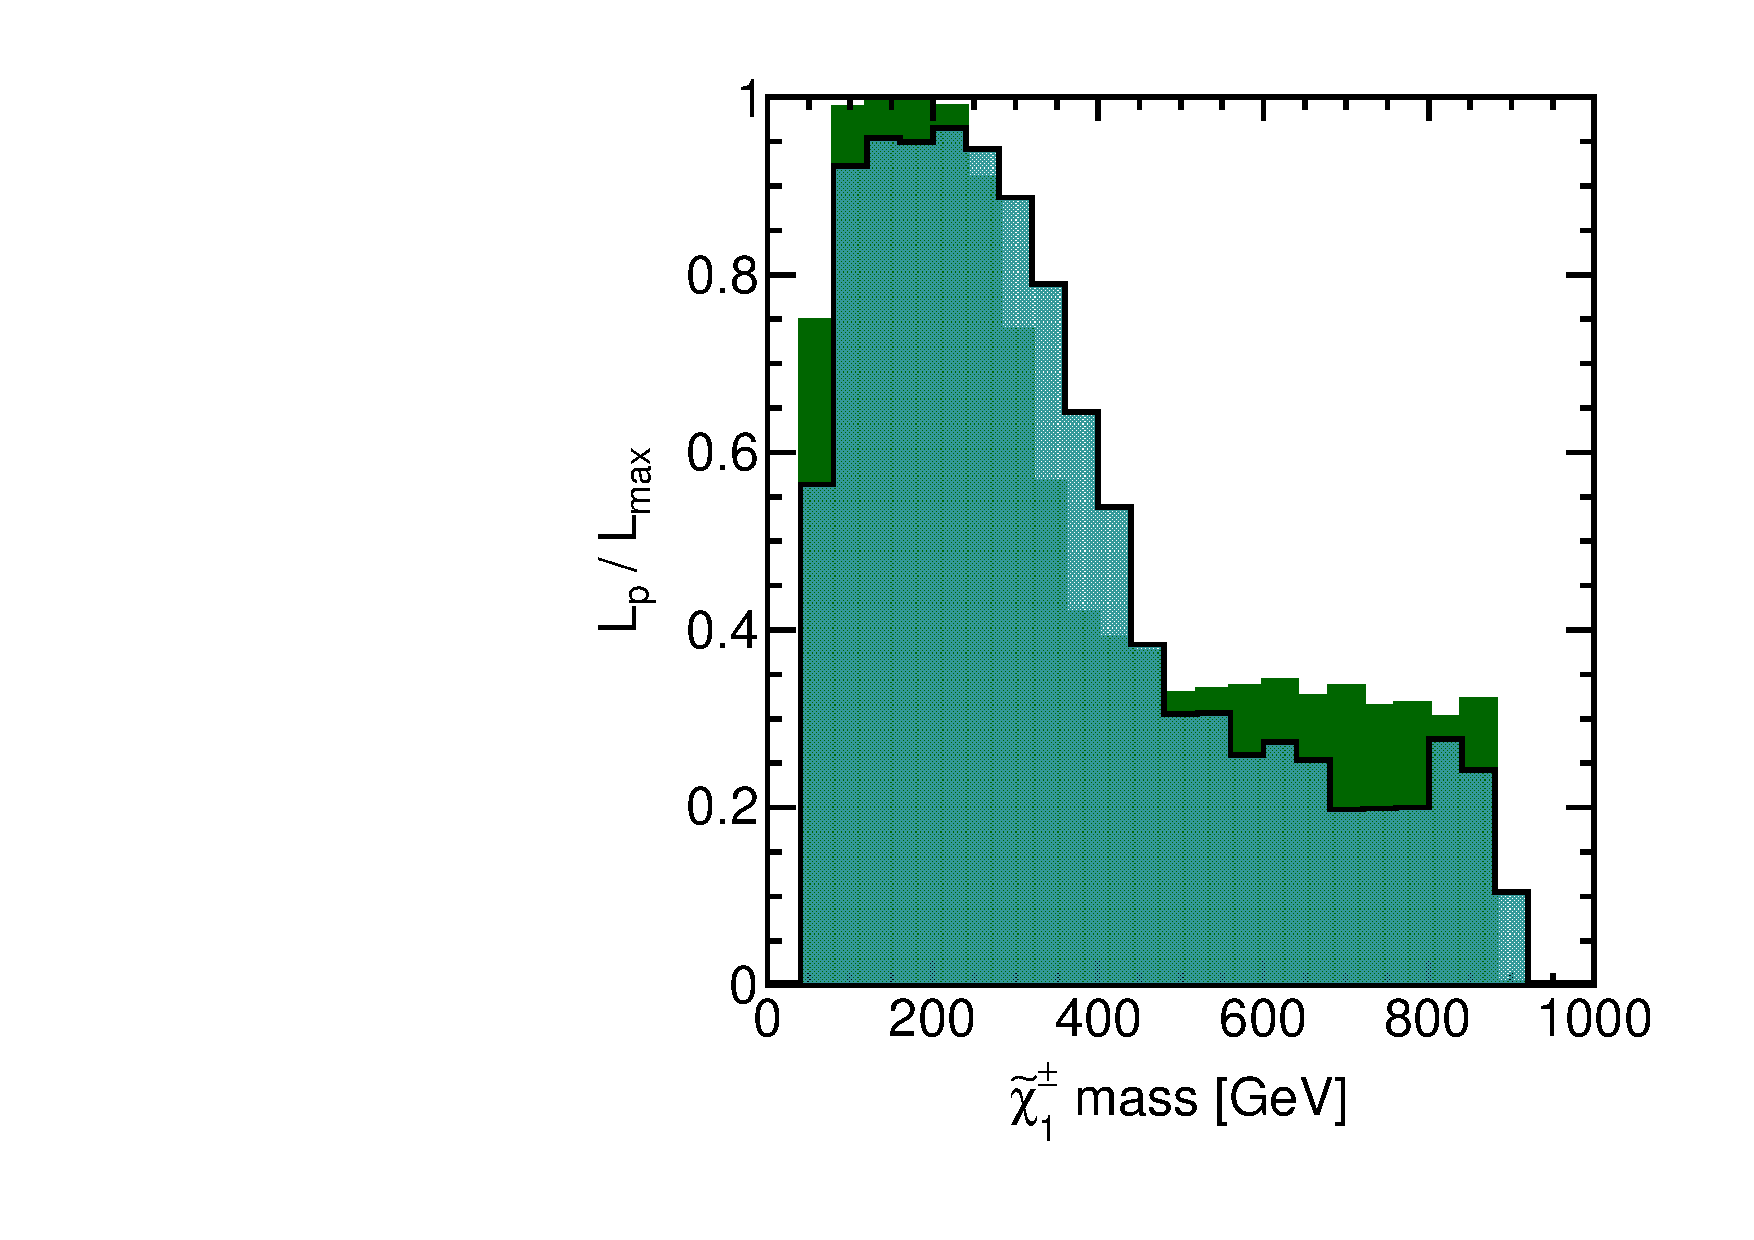
\includegraphics[height=5.5cm]{figs/fig_chi_1_pm.pdf} 
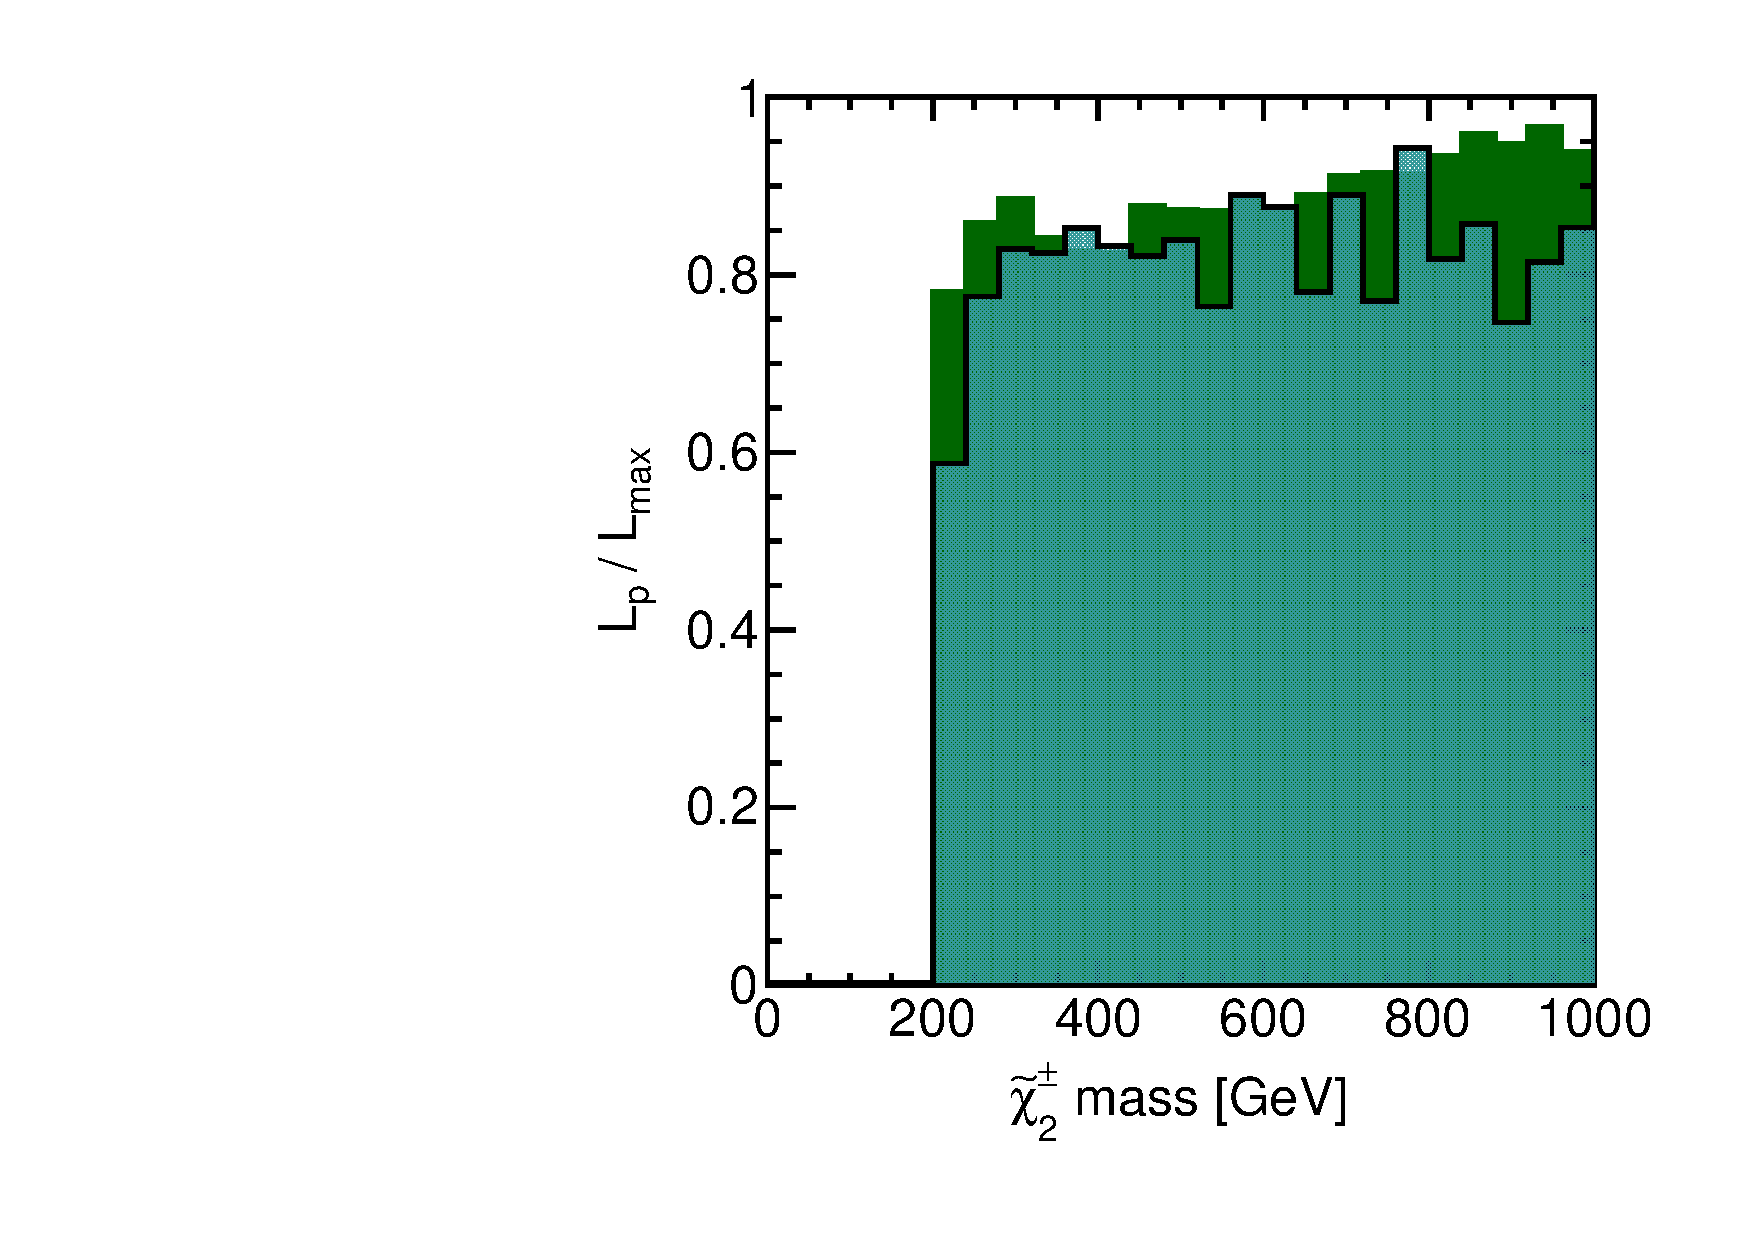
\includegraphics[height=5.5cm]{figs/fig_chi_2_pm.pdf}
\caption{Ratios of profile likelihood $L_p$ to maximum likelihood $L_{max}$ shown for chargino masses.  The colored and shaded histograms show the distributions before and after the inclusion of the CMS results.}
\label{fig:LRwcms_chipm}
\end{center}
\end{figure}


\begin{figure}[htbp]
\begin{center}
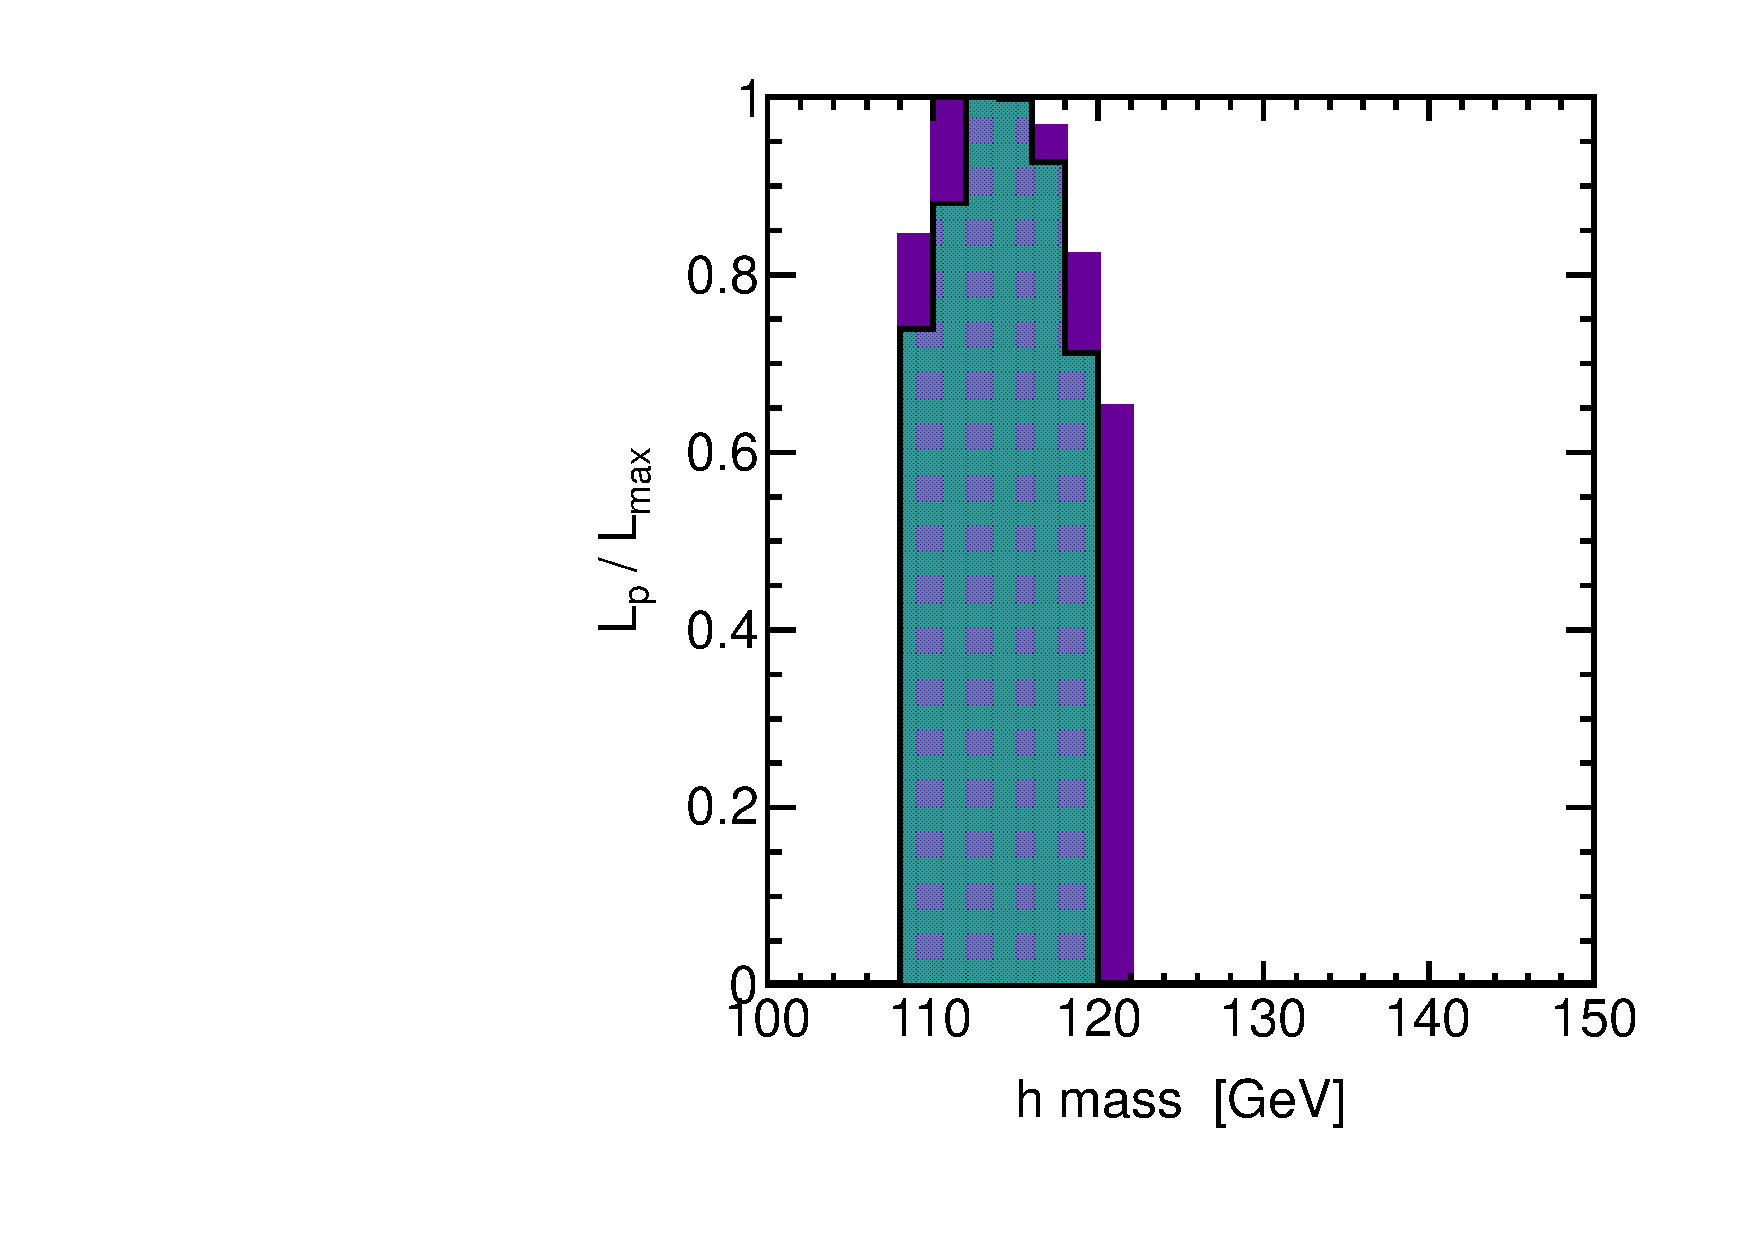
\includegraphics[height=5.5cm]{figs/fig_h.pdf} 
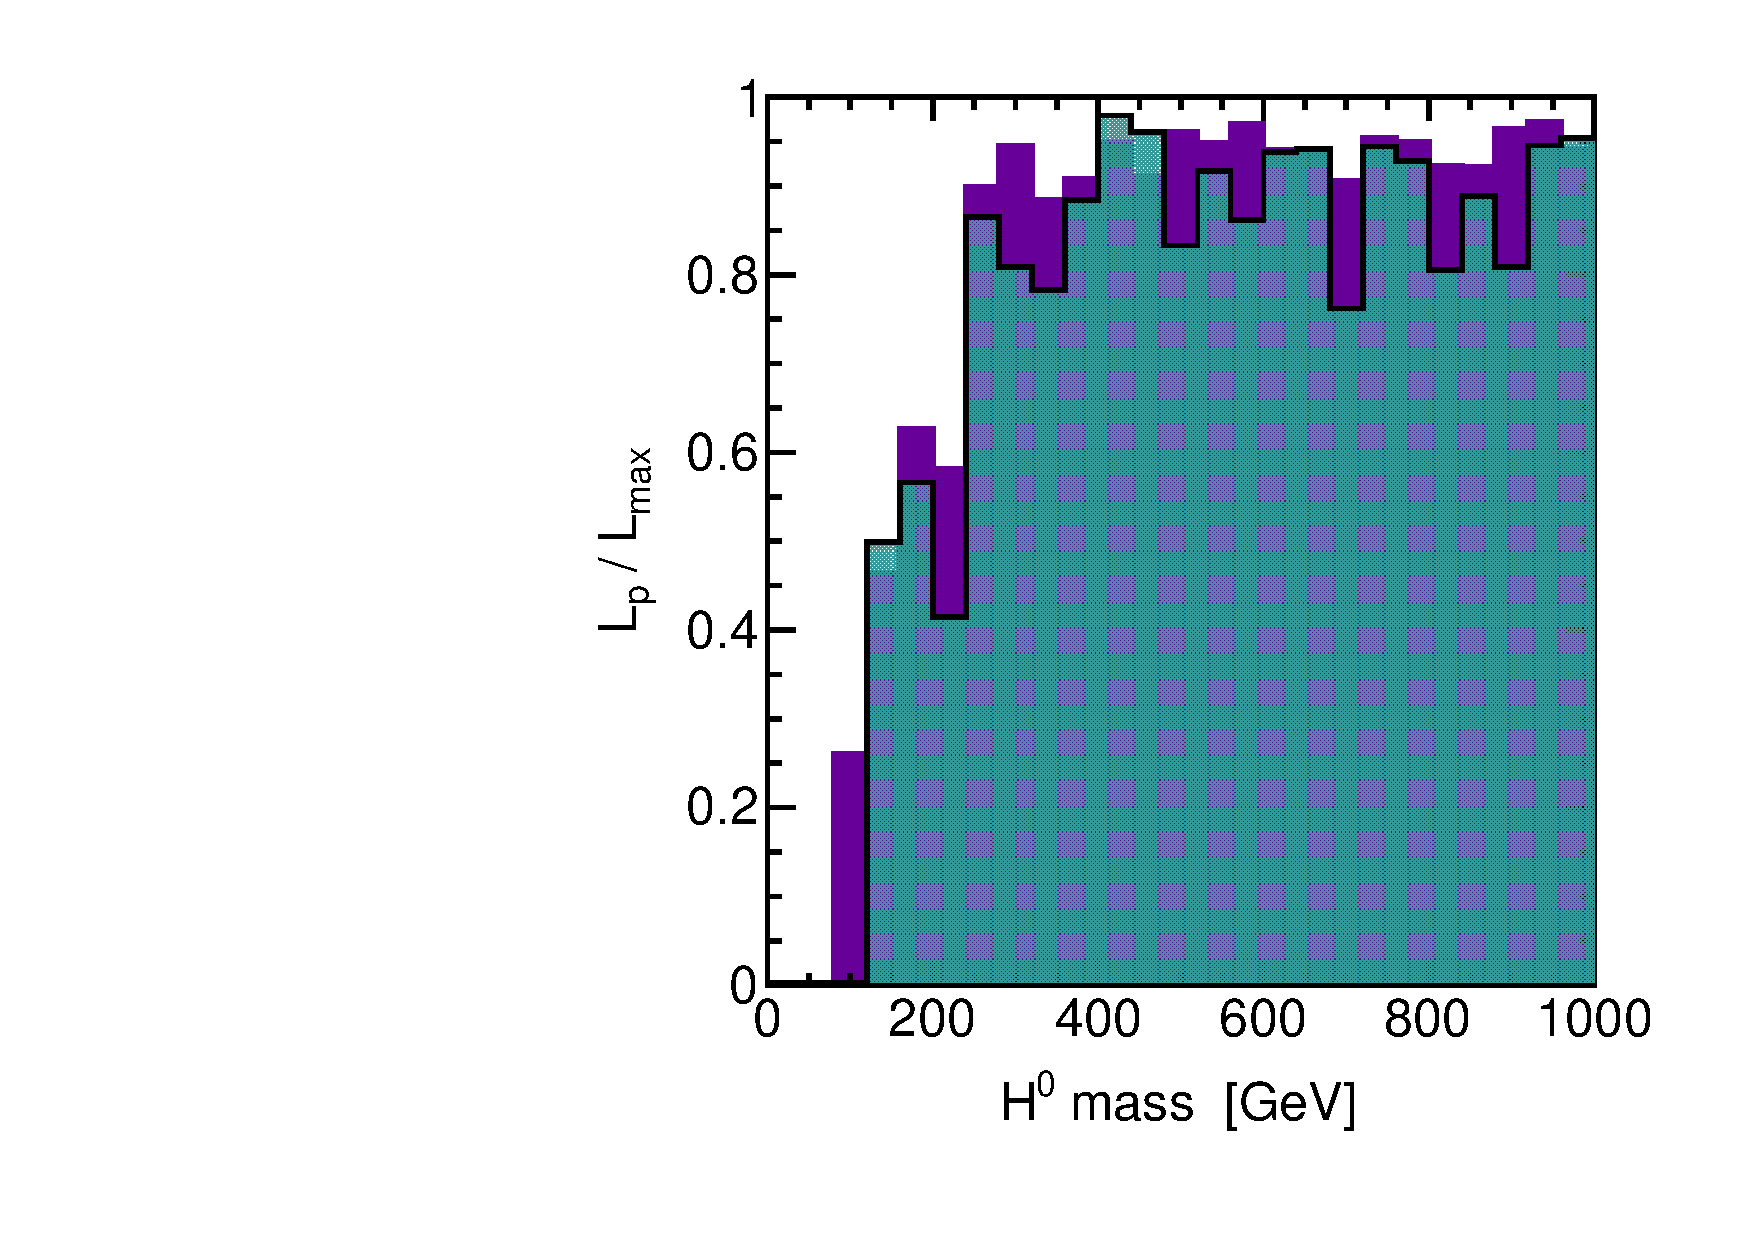
\includegraphics[height=5.5cm]{figs/fig_H0.pdf} \\
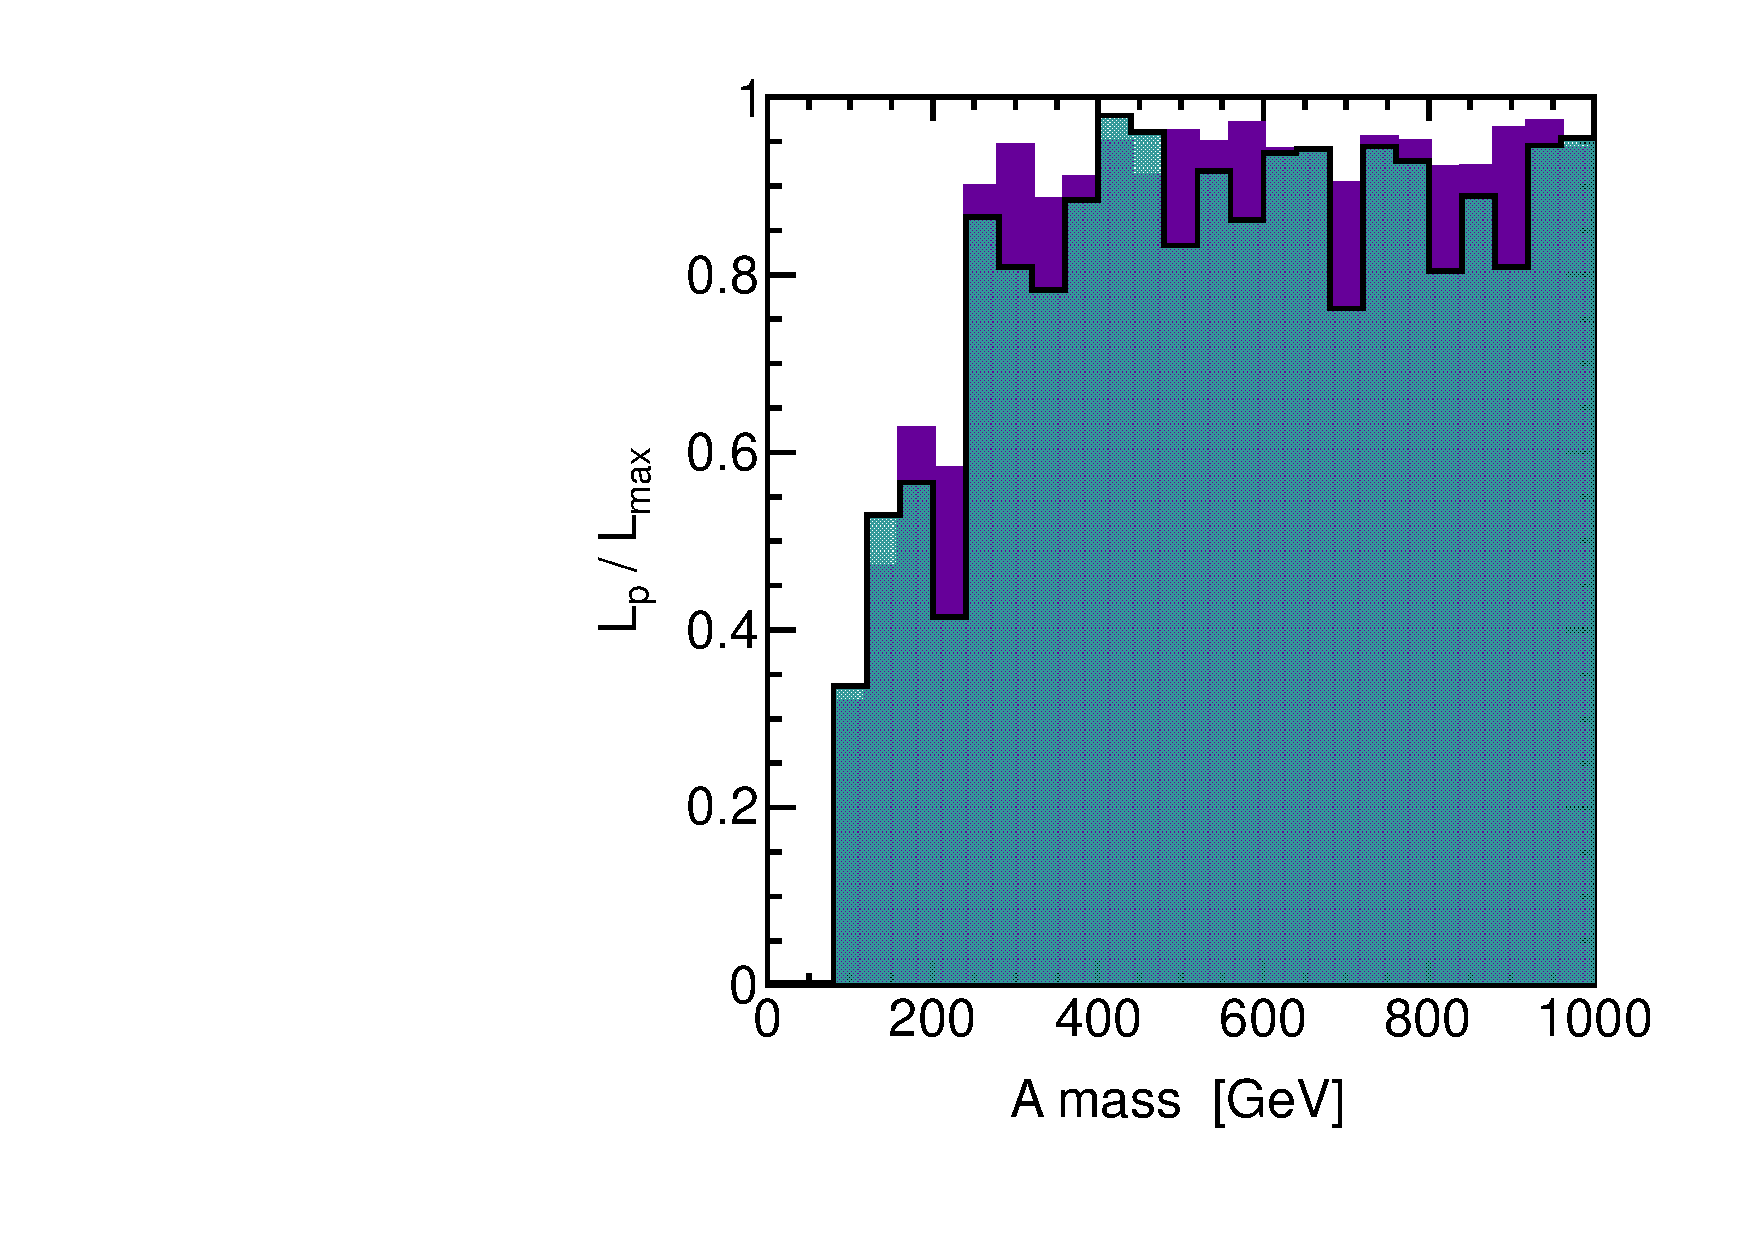
\includegraphics[height=5.5cm]{figs/fig_A.pdf} 
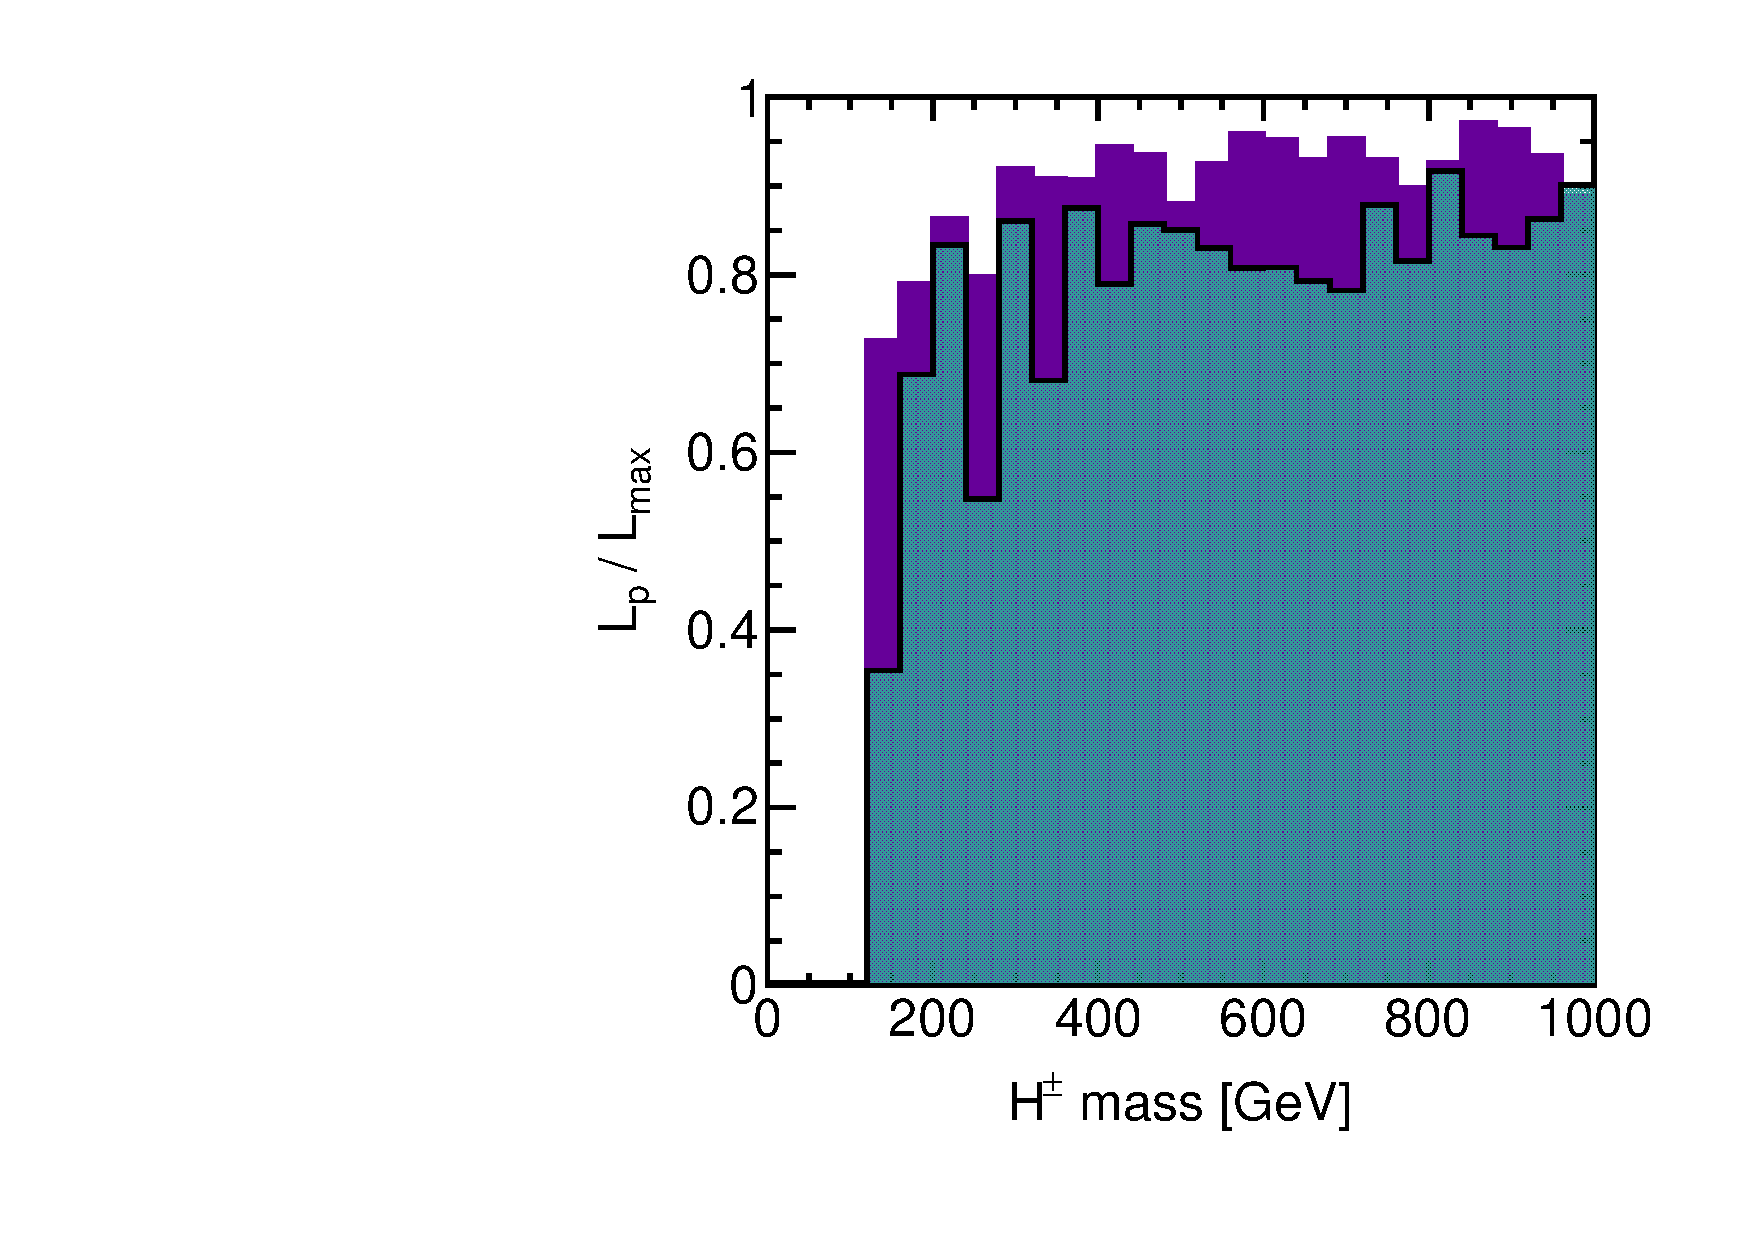
\includegraphics[height=5.5cm]{figs/fig_H_pm.pdf} 
\caption{Ratios of profile likelihood $L_p$ to maximum likelihood $L_{max}$ shown for the Higgs masses.  The colored and shaded histograms show the distributions before and after the inclusion of the CMS results.}
\label{fig:LRwcms_Higgs}
\end{center}
\end{figure}


\begin{figure}[htbp]
\begin{center}
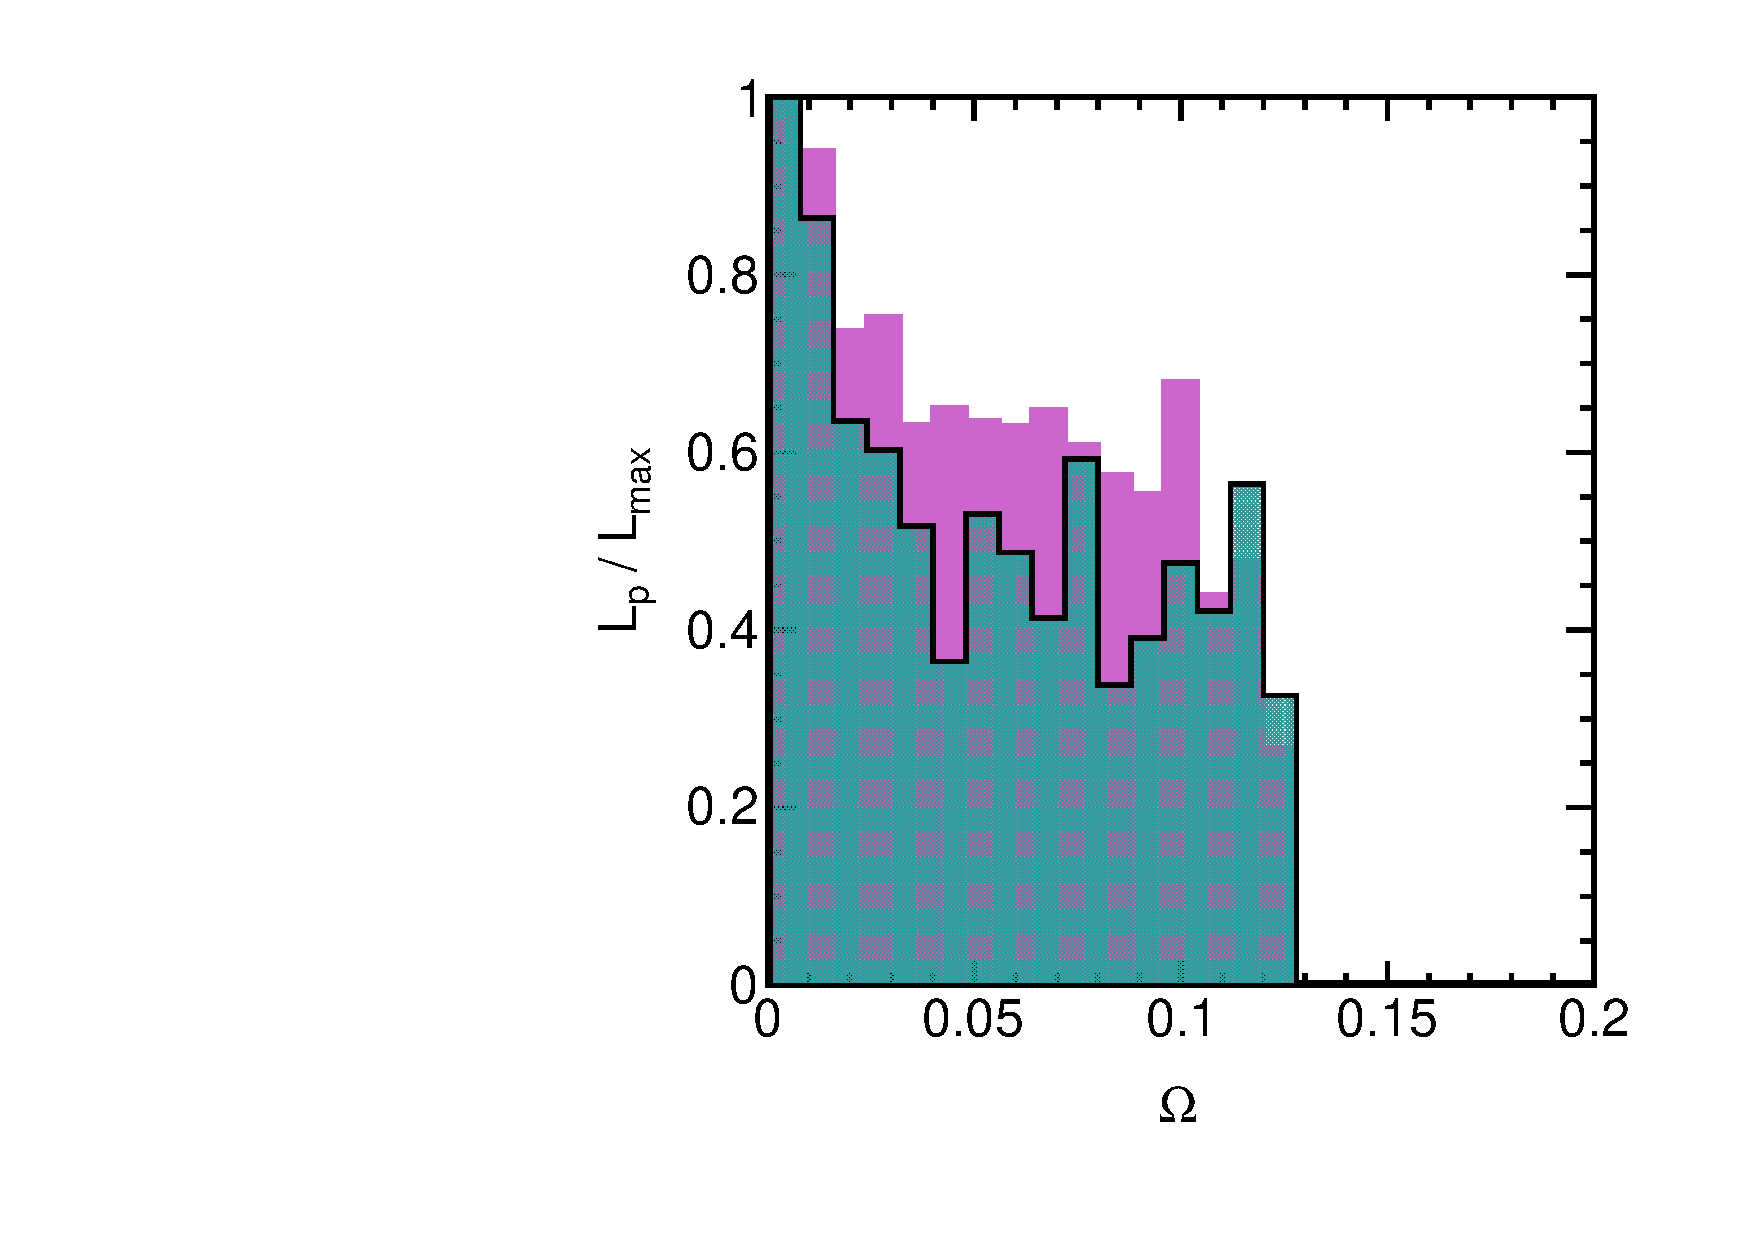
\includegraphics[height=5.5cm]{figs/fig_omega_m.pdf} 
\caption{Ratio of profile likelihood $L_p$ to maximum likelihood $L_{max}$ shown for lightest neutralino dark matter relic density.  The colored and shaded histograms show the distributions before and after the inclusion of the CMS results.}
\label{fig:LRwcms_omg}
\end{center}
\end{figure}


%\begin{figure}[htbp]
%\begin{center}
%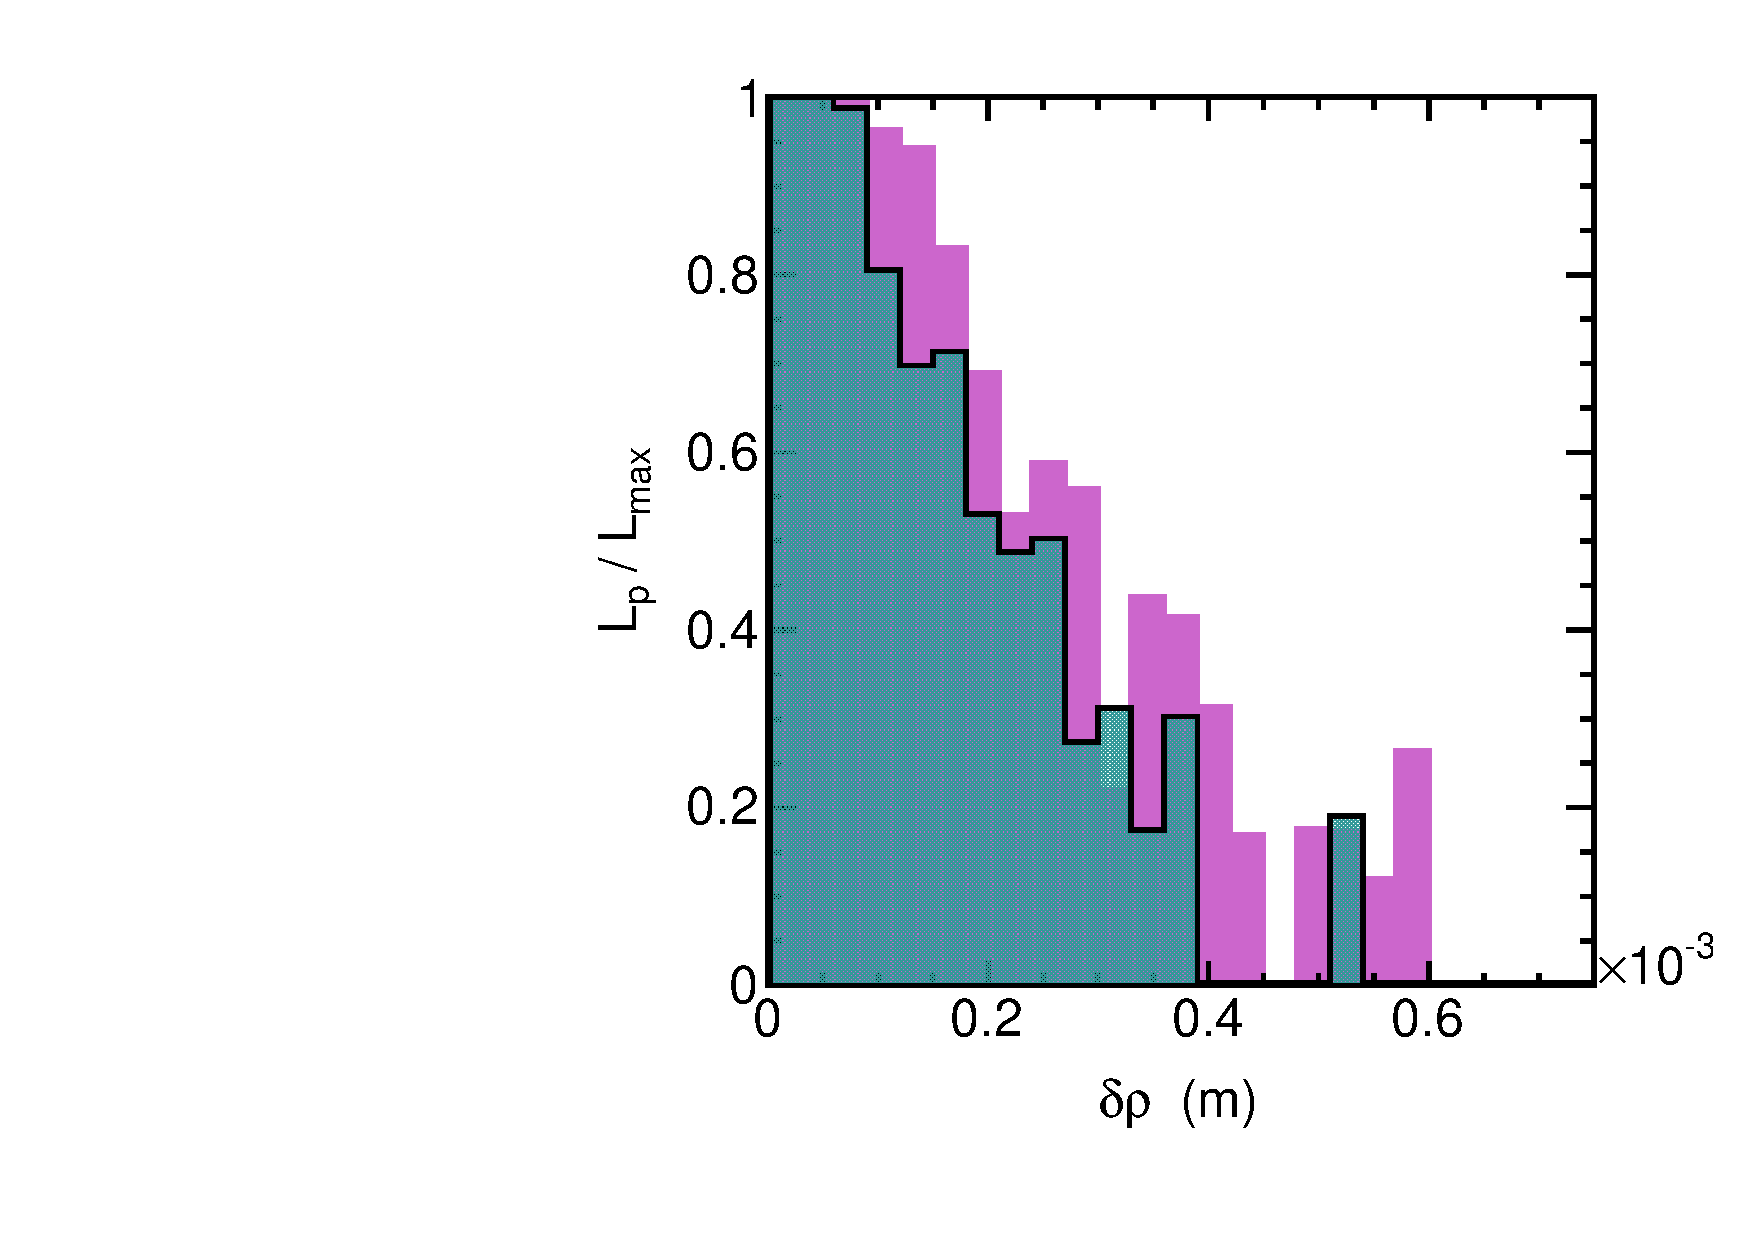
\includegraphics[height=5.5cm]{figs/fig_drho_m.pdf} 
%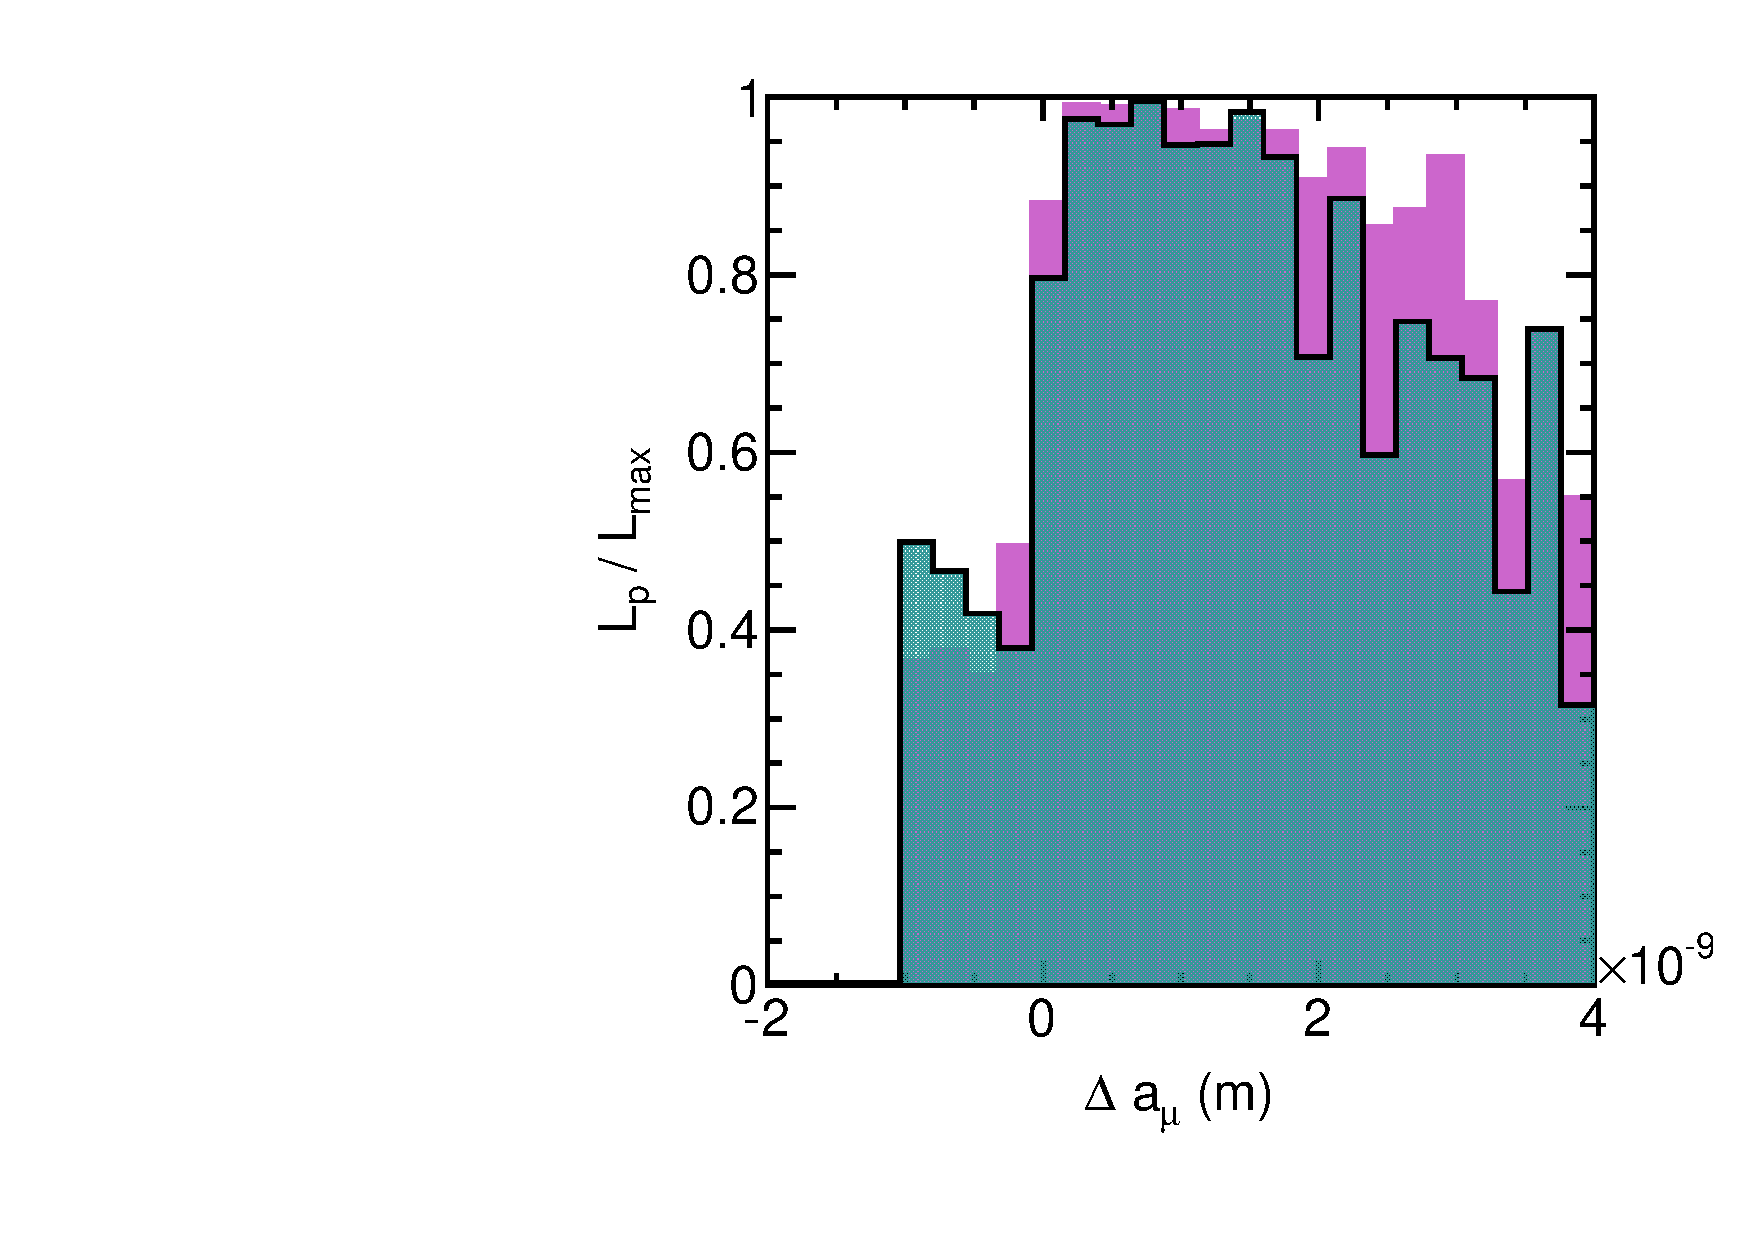
\includegraphics[height=5.5cm]{figs/fig_gmu_m.pdf} \\
%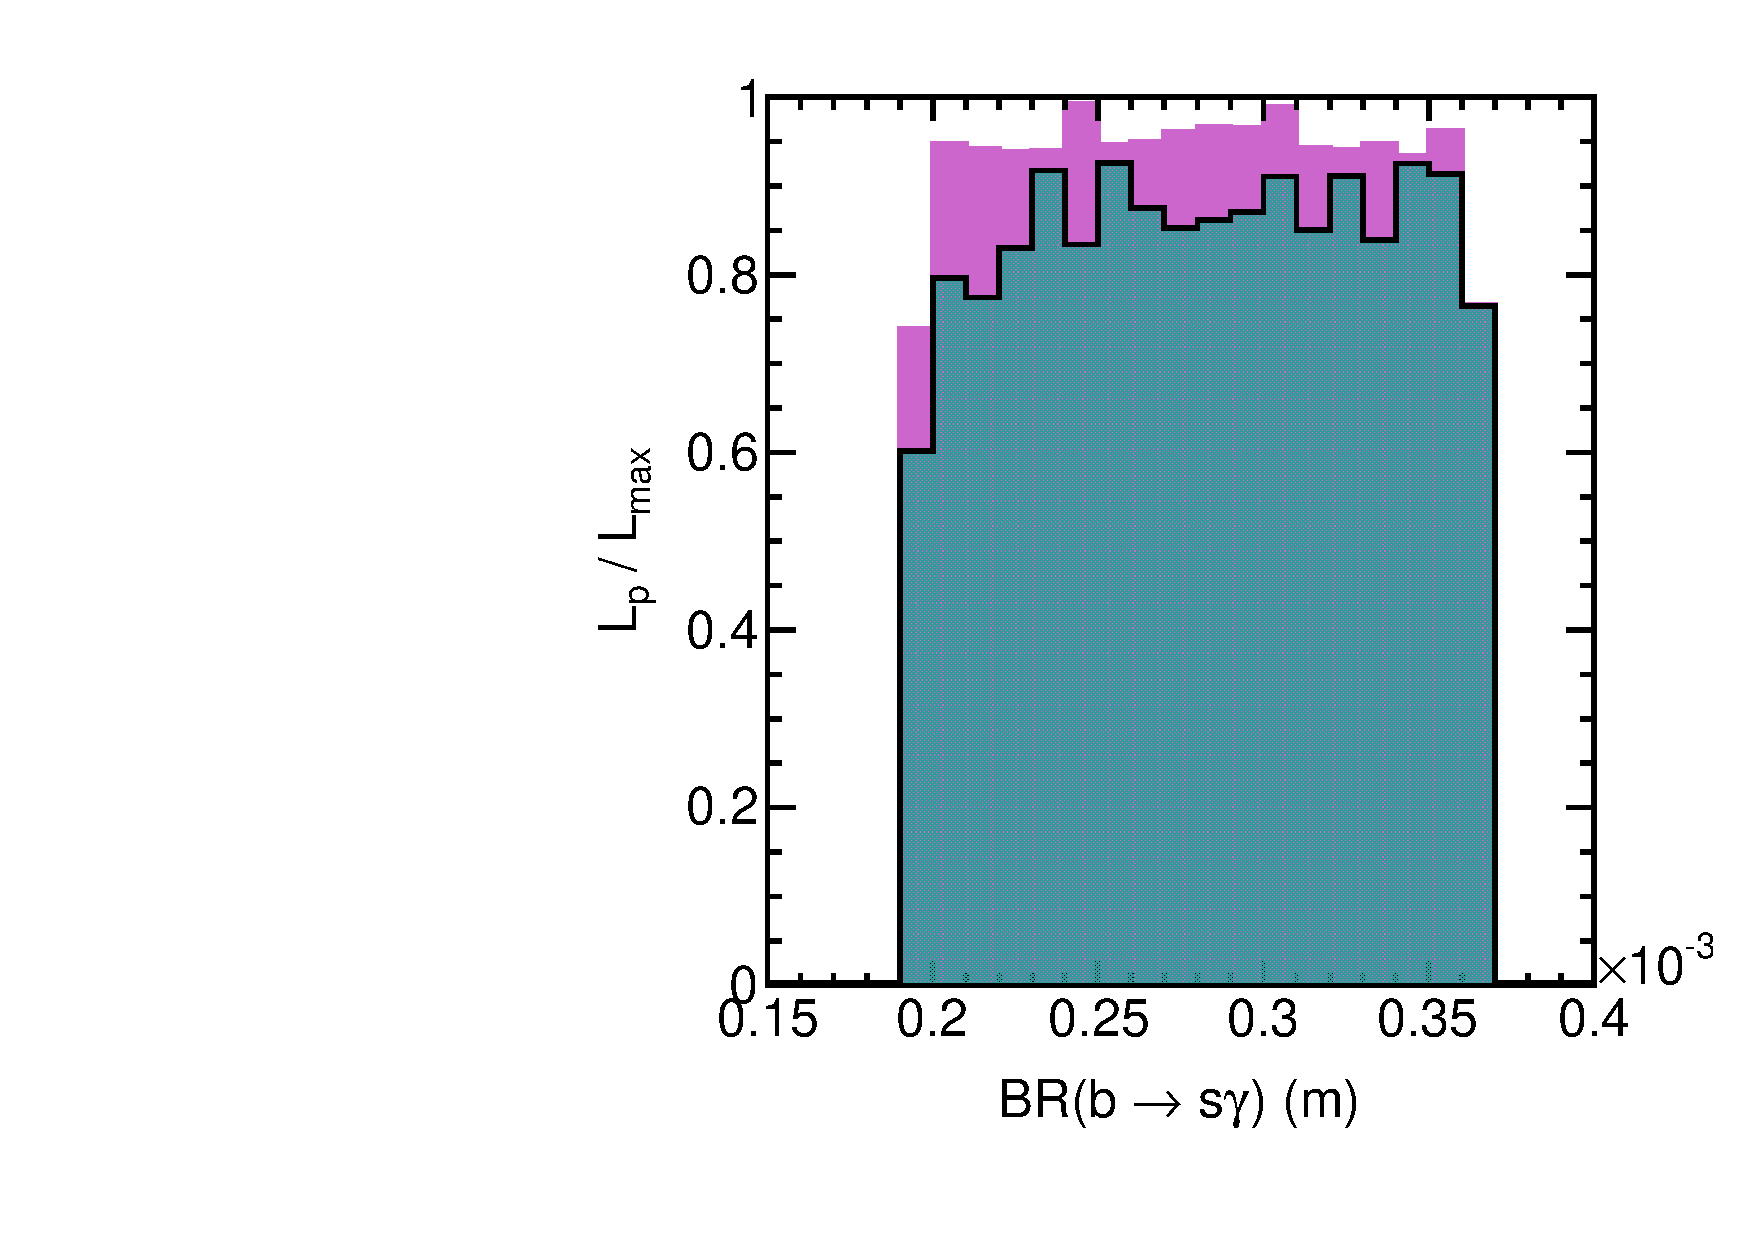
\includegraphics[height=5.5cm]{figs/fig_bsgamma_m.pdf} 
%\includegraphics[height=5.5cm]{figs/fig_bsmumu_m.pdf} \\
%\includegraphics[height=5.5cm]{figs/fig_rbtaunu_m.pdf} 
%\caption{Ratios of profile likelihood $L_p$ to maximum likelihood $L_{max}$ shown for predictions for weak scale observables as calculated by micromegas.  The colored and shaded histograms show the distributions before and after the inclusion of the CMS results.}
%\label{fig:LRwcms_EWobs_m}
%\end{center}
%\end{figure}


\begin{figure}[htbp]
\begin{center}
%\includegraphics[height=5.5cm]{figs/fig_delta0_s.pdf} 
\includegraphics[height=5.5cm]{figs/fig_drho_m.pdf} 
\includegraphics[height=5.5cm]{figs/fig_muon_gm2_s.pdf} \\
\includegraphics[height=5.5cm]{figs/fig_bsgamma_s.pdf} 
\includegraphics[height=5.5cm]{figs/fig_Bsmumu_s.pdf} \\
\includegraphics[height=5.5cm]{figs/fig_Btaunu_s.pdf} 
\includegraphics[height=5.5cm]{figs/fig_RBtaunu_s.pdf} 
\caption{Ratios of profile likelihood $L_p$ to maximum likelihood $L_{max}$ shown for predictions for weak scale observables.  $\delta\rho$ is calculated using {\tt micrOMEGAs 2.4} and the rest are calculated using {\tt Superiso 2.7}.  The colored and shaded histograms show the distributions before and after the inclusion of the CMS results.}
\label{fig:LRwcms_EWobs_s1}
\end{center}
\end{figure}


\begin{figure}[htbp]
\begin{center}
\includegraphics[height=5.5cm]{figs/fig_BDtaunu_s.pdf} 
\includegraphics[height=5.5cm]{figs/fig_BDtaunu_BDenu_s.pdf} \\
\includegraphics[height=5.5cm]{figs/fig_Dmunu_s.pdf} 
\includegraphics[height=5.5cm]{figs/fig_Dsmunu_s.pdf} \\
\includegraphics[height=5.5cm]{figs/fig_Dstaunu_s.pdf} 
\includegraphics[height=5.5cm]{figs/fig_Kmunu_pimunu_s.pdf} \\
\includegraphics[height=5.5cm]{figs/fig_Rl23_s.pdf} 
\caption{Ratios of profile likelihood $L_p$ to maximum likelihood $L_{max}$ shown for predictions for weak scale observables as calculated by {\tt Superiso 2.7}.  The colored and shaded histograms show the distributions before and after the inclusion of the CMS results.}
\label{fig:LRwcms_EWobs_s2}
\end{center}
\end{figure}






\section{Conclusion}
\label{sec:conclusion}

We have assessed the sensitivity to mSUGRA of a generic signal characterized by two isolated, high $p_T$ leptons,
significant jet activity, and \met. We performed a scan of the mSUGRA $m_{0}-m_{1/2}$ parameter space and determined  
the expected excluded region in the case of no observed signal as well as the $5\sigma$ sensitivity reach for both SS
and OS dileptons, assuming integrated luminosities of 100 pb$^{-1}$ and 1 fb$^{-1}$. Our results indicate that we are sensitive to a
significant region of the mSUGRA parameter space which extends upon previous results from the Tevatron. 




\clearpage
\begin{thebibliography}{10}

\bibitem{Choi:2007ka}
K.~Choi and H.~P. Nilles,
\newblock JHEP {\bf 04}, 006 (2007), hep-ph/0702146.

\bibitem{Martin:2009ad}
S.~P. Martin,
\newblock Phys. Rev. {\bf D79}, 095019 (2009), 0903.3568.

\bibitem{Horton:2009ed}
D.~Horton and G.~G. Ross,
\newblock Nucl. Phys. {\bf B830}, 221 (2010), 0908.0857.

\bibitem{Allanach:2006fy}
B.~C. Allanach {\em et~al.},
\newblock (2006), hep-ph/0602198.

\bibitem{Kolda:1995iw}
C.~F. Kolda and S.~P. Martin,
\newblock Phys. Rev. {\bf D53}, 3871 (1996), hep-ph/9503445.

\bibitem{Polonsky:1994sr}
N.~Polonsky and A.~Pomarol,
\newblock Phys. Rev. Lett. {\bf 73}, 2292 (1994), hep-ph/9406224.

\bibitem{Polonsky:1994rz}
N.~Polonsky and A.~Pomarol,
\newblock Phys. Rev. {\bf D51}, 6532 (1995), hep-ph/9410231.

\bibitem{Ellis:2002wv}
J.~R. Ellis, K.~A. Olive, and Y.~Santoso,
\newblock Phys. Lett. {\bf B539}, 107 (2002), hep-ph/0204192.

\bibitem{Berger:2008cq}
C.~F. Berger, J.~S. Gainer, J.~L. Hewett, and T.~G. Rizzo,
\newblock JHEP {\bf 02}, 023 (2009), 0812.0980.

\bibitem{Conley:2010du}
J.~A. Conley, J.~S. Gainer, J.~L. Hewett, M.~P. Le, and T.~G. Rizzo,
\newblock (2010), 1009.2539.

\bibitem{Lyons:2003bw}
L.~Lyons, (ed.~), R.~P. Mount, (ed.~), and R.~Reitmeyer, (ed.~),
\newblock Prepared for PHYSTAT2003: Statistical Problems in Particle Physics,
  Astrophysics, and Cosmology, Menlo Park, California, 8-11 Sep 2003.

\bibitem{Nakamura:2010zzi}
Particle Data Group, K.~Nakamura,
\newblock J. Phys. {\bf G37}, 075021 (2010).

\bibitem{top:1900yx}
CDF and D0, and others,
\newblock (2010), 1007.3178.

\bibitem{Schael:2006cr}
{ALEPH, DELPHI, L3 and OPAL collaborations and the LEP Working Group for Higgs
  Boson Searches}, S.~Schael {\em et~al.},
\newblock Eur. Phys. J. {\bf C47}, 547 (2006), hep-ex/0602042.

\bibitem{Degrassi:2002fi}
G.~Degrassi, S.~Heinemeyer, W.~Hollik, P.~Slavich, and G.~Weiglein,
\newblock Eur. Phys. J. {\bf C28}, 133 (2003), hep-ph/0212020.

\bibitem{Davier:2010nc}
M.~Davier, A.~Hoecker, B.~Malaescu, and Z.~Zhang,
\newblock (2010), 1010.4180.

\bibitem{HFAG:2010qj}
The Heavy Flavor Averaging Group, D.~Asner {\em et~al.},
\newblock (2010), 1010.1589.

\bibitem{Jarosik:2010iu}
N.~Jarosik {\em et~al.},
\newblock (2010), 1001.4744.

\bibitem{lepsusy}
ALEPH, DELPHI, L3 and OPAL, {LEP2 SUSY Working Group,},
\newblock {\tt http://lepsusy.web.cern.ch/lepsusy/}.

%\cite{Skands:2003cj}
\bibitem{Skands:2003cj}
  P.~Z.~Skands {\it et al.},
  %``SUSY Les Houches Accord: Interfacing SUSY Spectrum Calculators, Decay
  %Packages, and Event Generators,''
  JHEP {\bf 0407} (2004) 036
  [arXiv:hep-ph/0311123].
  %%CITATION = JHEPA,0407,036;%%

%\cite{Sjostrand:2006za}
\bibitem{Sjostrand:2006za}
  T.~Sjostrand, S.~Mrenna and P.~Z.~Skands,
  %``PYTHIA 6.4 Physics and Manual,''
  JHEP {\bf 0605} (2006) 026
  [arXiv:hep-ph/0603175].
  %%CITATION = JHEPA,0605,026;%%

%\cite{Ovyn:2009tx}
\bibitem{Ovyn:2009tx}
  S.~Ovyn, X.~Rouby and V.~Lemaitre,
  %``Delphes, a framework for fast simulation of a generic collider
  %experiment,''
  arXiv:0903.2225 [hep-ph].
  %%CITATION = ARXIV:0903.2225;%%
%
\bibitem{Belanger:2006is}
  G.~Belanger, F.~Boudjema, A.~Pukhov and A.~Semenov,
  %``micrOMEGAs2.0: A program to calculate the relic density of dark matter  in
  %a generic model,''
  Comput.\ Phys.\ Commun.\  {\bf 176}, 367 (2007)
  [arXiv:hep-ph/0607059].
  %%CITATION = CPHCB,176,367;%%
%
\bibitem{Mahmoudi:2008tp}
  F.~Mahmoudi,
  %``SuperIso v2.3: A Program for calculating flavor physics observables in
  %Supersymmetry,''
  Comput.\ Phys.\ Commun.\  {\bf 180}, 1579 (2009)
  [arXiv:0808.3144 [hep-ph]].
  %%CITATION = CPHCB,180,1579;%%
%


\end{thebibliography}

\end{document}
